\chapter{جبری‌سازی و استخراج معادلات سامانه‌های رمزنگاری}
در این فصل ثابت می‌کنیم که نه تنها نگاشت‌های رمزنگاری بلکه هر نگاشت از یک مجموعه‌ی متناهی به یک مجموعه‌ی متناهی دیگر  را می‌توان به صورت یک نگاشت چندجمله‌ای روی یک میدان متناهی  بیان کرد، به این ترتیب شکستن یک سامانه‌ی رمزنگاری به مسئله‌ی حلّ دستگاه معادلات چندجمله‌ای تبدیل می‌شود. پس از تعریف دقیق حمله‌  جبری با سناریوهای مختلف حمله‌ی جبری روی انواع سامانه‌های رمزنگاری آشنا می‌شویم و در انتها مثال‌هایی واقعی از تبدیل سامانه‌های رمزنگاری به دستگاه معادلات چندجمله‌ای روی میدان متناهی را خواهیم دید. بخش زیادی از مباحث این فصل برگرفته از 
\cite{bard2009algebraic}، 
است که یکی از مراجع مفید در زمینه‌ حمله‌های جبری محسوب می‌شود.
\section{نگاشت‌های عام}
هدف از این بخش این است که ثابت کنیم، هر نگاشت رمزنگاری را می‌توان به صورت نگاشتی چندجمله‌ای روی یک میدان متناهی بیان کرد، امّا نحوه‌  به‌دست آوردن آن موضوعی است که در بخش‌های بعدی بررسی می‌شود. 

\begin{lemma}
	\label{unimaplem1}
	فرض کنید 
$\mathbb{F}$
یک میدان متناهی از مرتبه‌ی عدد اوّل 
$p$
باشد، در این صورت هر نگاشت از 
$\mathbb{F}$
-فضای برداری متناهی بعد 
$V$
 به میدان 
 $\mathbb{F}$
 را می توان به صورت یک نگاشت چندجمله‌ای با ضرایب در 
 $\mathbb{F}$
 نوشت.
 
 \begin{proof}
 	می‌دانیم مجموعه‌ی همه‌ی نگاشت‌ها از 
 	$V$
 	به 
 	$\mathbb{F}$
 	یک 
 	$\mathbb{F}$
-فضای برداری است، که آن را با 
 	$\varPhi$
 	نمایش می‌دهیم. برای اثبات حکم، پایه‌ای برای این فضای برداری ارائه می‌دهیم که همه‌ی اعضایش چندجمله‌ای‌هایی با ضرایب در 
 	$\mathbb{F}$
 	هستند. مجموعه‌ی 
 		$B:=\{\varphi_{x}:V\ra \mathbb{F} \ | \ x\in V\}$
 	 که برای هر 
 	$x\in V$
 	نگاشت 
 	$\varphi_{x}:V\ra \mathbb{F}$
 	را به صورت زیر تعریف می‌کنیم:
\begin{equation*}
\varphi_{x}(y):=
\left\{
\begin{array}{lr}
1   & y = x \\‎ 
0  & y\neq x
\end{array}\right.
\end{equation*}
 در نظر بگیرید. نگاشت دلخواه  
 $\varphi\in\varPhi$
را می‌توان به‌صورت زیر نوشت:
$$\varphi = \sum_{x\in V}\varphi(x)*\varphi_{x}$$
بنابراین 
$B$
 مولدی برای 
 $V$
 است، از طرفی به ازای 
 $x_{0}\in V$
 دلخواه، 
 $B\backslash\{\varphi_{x_{0}}\}$
 یک مولّد 
 $\varPhi$
 نیست، زیرا 
 $\varphi_{x_{0}}$
 را نمی‌توان به صورت ترکیب 
 $\mathbb{F}$
 خطّی از اعضای 
 $B\backslash\{x_{0}\}$
 نوشت. بنابراین  
 $B$
 یک مولّد مینیمال و لذا یک پایه 
 $\mathbb{F}$
 -فضای برداری 
 $\varPhi$
 است. چون میدان 
 $\mathbb{F}$
 و در نتیجه فضای برداری 
 $V$
 متناهی است، کافی است نشان دهیم هر یک از  
 $\varphi_{x}$
 ها یک 
 $\mathbb{F}$
-چندجمله‌ای است. بُعد 
$V$
برابر با 
$n$
 و 
$x = (x_{1},..., x_{n})\in V$
را دلخواه و از این پس ثابت فرض کنید. 
$\mathbb{F}$
 یک میدان است، بنابراین 
 $(x_{i}-y_{i})^{p-1} - 1 \neq 0$
  اگر و تنها اگر 
  $x_{i} = y_{i}$.  
در نتیجه چندجمله‌ای زیر همه‌جا به جز در 
$x$
برابر صفر است:
$$\fa \ y = (y_{1},..., y_{n})\in V: \ \psi_{x}(y_{1},..., y_{n}) := \Pi_{i = 1}^{n}((x_{i}-y_{i})^{p-1} - 1)$$
با توجّه به تعریف 
$\psi_{x}$
داریم:
$$\fa y = (y_{1},...,y_{n})\in V : \ \varphi_{x}(y) = \frac{\psi_{x}(y_{1},..., y_{n})}{\psi_{x}(x_{1},..., x_{n})}.$$
چون 
$x\in V$
ثابت فرض شده بود مخرج نگاشت فوق یک مقدار ثابت و لذا 
$\varphi_{x}$
یک چندجمله‌ای 
$n$
متغیره بر حسب 
$y_{1},..., y_{n}$
است و در نهایت چون 
$x\in V$
را دلخواه انتخاب کرده بودیم حکم ثابت می‌شود.
 \end{proof}
\end{lemma}

\begin{lemma}
اگر 
$\mathbb{F}$
یک میدان متناهی با مشخصه‌ی عدد اوّل 
$p$
باشد، هر نگاشت از یک 
$\mathbb{F}$-
فضای برداری متناهی بعد مثل 
$V$
به 
$\mathbb{GF}(p)$
را می‌توان به صورت چندجمله‌ای با ضرایب در 
$\mathbb{GF}(p)$
نوشت.

\begin{proof}
$\mathbb{F}$
یک میدان متناهی با مشخصه‌ی 
$p$
است، لذا بدون کاستن از کلیت فرض می‌کنیم 
$\mathbb{F} = \mathbb{GF}(p^{n})$
که 
$n\in \mathbb{N}$.
 بنابراین  
 $\mathbb{F}$
 یک فضای برداری از بعد 
 $n$
 روی 
 $\mathbb{GF}(p)$
 نیز خواهد بود که ضرب اسکالر آن به صورت زیر تعریف می‌شود.
 	$$* :\mathbb{GF}(p)\rightarrow \mathbb{F}$$
 	$$(k,x)\mapsto k.x = x+x+\cdots+x  \ (\text{بار}k)$$
بُعد
$V$
را برابر عدد طبیعی 
$m$
در نظر می‌گیریم. در نتیجه 
$V$
یک فضای برداری 
$m*n$
بعدی روی میدان
$\mathbb{GF}(p)$
است و طبق لم قبل حکم ثابت می‌شود.
\end{proof}
\end{lemma}

\begin{lemma}
اگر 
$\mathbb{F}$
یک میدان متناهی با مشخصه‌ی عدد اوّل 
$p$
باشد، هر نگاشت از 
$\mathbb{F}$-
فضای برداری متناهی بُعد 
$V$
به 
$\mathbb{GF}(p)$-
فضای برداری متناهی بُعد 
$U$
 یک نگاشت چندجمله‌ای با ضرایب در
 $\mathbb{GF}(p)$
 است، یعنی با فرض 
 $dim(V) = n$
 و 
 $dim(U) = m$
 برای هر نگاشت 
 $f:V\ra U$
 داریم
 $$\exi \ f_{1},...,f_{m}\in\mathbb{GF}(p)[x_{1},...,x_{n}] \  \ f(x_{1},...,x_{n}) = (f_{1}(x_{1},...,x_{n}),..., f_{m}(x_{1},..., x_{n})).$$
 که 
 $f_{i}\in\mathbb{GF}(p)[x_{1},..., x_{n}]$
 برای هر 
 $i = 1,...,m$.
 \begin{proof}
 	چون 
 	$V$
 	یک 
 	$\mathbb{F}$-
 	فضای برداری با بعد 
 	$n$
 	 و 
 	 $\mathbb{F}$
 	 یک میدان متناهی با مشخصه‌ی عدد اوّل 
 	 $p$
 	 است، طبق لم قبل هر یک از توابع مؤلفه‌ای 
 	 $f_{i}$
 	 که 
 	 $i = 1,...,m$
 	 یک چندجمله‌ای است و حکم ثابت می‌شود.
 \end{proof}
\end{lemma}

\begin{lemma}
	\label{unimaplem4}
فرض کنید 
$\mathbb{F}$
و 
$\mathbb{G}$
دو میدان متناهی با مشخصه‌ی عدد اوّل 
$p$
باشند، در این‌صورت هر نگاشت از 
$\mathbb{F}$-
فضای برداری متناهی بُعد 
$V$
به 
$\mathbb{G}$-
فضای برداری متناهی بُعد 
$U$
 یک نگاشت چند‌جمله‌ای است.
 \begin{proof}
بدون کاستن از کلیت فرض می‌کنیم 
$\mathbb{G} = \mathbb{G}(p^{m})$
و 
$U = \mathbb{GF}(p^{m})^{n}$
که 
$m$
و
$n$
اعدادی طبیعی هستند. در نتیجه 
$U$
یک فضای برداری 
$m*n$
بعدی روی 
$\mathbb{GF}(p)$
است و طبق لم قبل حکم ثابت می‌شود.
 \end{proof}
\end{lemma}

\begin{theorem}[\textbf{نگاشت عام}]
\label{unimap th}
هر نگاشت از مجموعه‌ی متناهی 
$S$
به مجموعه‌ی متناهی 
$T$
را می‌توان به‌صورت یک نگاشت چند جمله‌ای روی 
$\mathbb{GF}(p)$
که 
$p$
یک عدد اوّل دلخواه است نوشت.

\begin{proof}
$p$
را یک عدد اوّل دلخواه در نظر بگیرید. اعداد طبیعی 
$m$
و
$n$
را طوری در نظر می‌گیریم که 
$p^{m}\geq |S|$
و
$p^{n}\geq|T|$.
سپس 
$S$
را در 
$\mathbb{GF}(p^{n})$
می‌نشانیم یا به بیان ساده‌تر اعضای 
$S$
را با اعضای 
$\mathbb{GF}(p^{n})$
برچسب‌گذاری می‌کنیم به همین ترتیب 
$T$
را در 
$\mathbb{GF}(p^{m})$
می‌نشانیم. اکنون می‌توانیم هر نگاشت دلخواه مثل 
$f:S\ra T$
را به صورت زیر به یک نگاشت روی 
$\mathbb{GF}(p^{n})$
توسعه می‌دهیم.
	$$F:\mathbb{GF}(p^n)\rightarrow \mathbb{GF}(p^m)$$
	$$F(x) = \left \{ \begin{array}{ll}
	f(x) & x\in S\\
	y_0 & o.w
	\end{array} \right.
	$$
	که 
	$y_{0}\in\mathbb{GF}(p^{m})$
	یک عضو دلخواه و ثابت است. طبق لم 
	\ref{unimaplem4}
	نگاشت فوق چندجمله‌ای است و در نتیجه تحدید آن به 
	$S$
	(یا مجموعه‌ی متناظر با آن در 
	$\mathbb{GF}(p^{n})$
	)
که آن را با 
$F|_{S} = f$
نمایش می‌دهیم نیز چندجمله‌ای است.
\end{proof}
\end{theorem}

قضیه‌ی فوق این اطمینان را می‌دهد که هر نگاشت (رمزنگاری) را می‌توان به‌صورت چندجمله‌ای بیان کرد ولی روش به‌دست آوردن این نمایش را در اختیار ما قرار نمی‌دهد. در ادامه پس از معرفی حمله‌های جبری الگوریتمی را معرفی می‌کنیم که می‌تواند در تبدیل  نگشات‌های رمزنگاری به نگاشت چندجمله‌ای مورد استفاده قرار گیرد. 
\section{حمله‌ی جبری چیست؟}
پروتکل‌های رمزنگاری که هسته‌ی اصلی تشکیل‌دهنده‌  آن‌ها سامانه‌های رمزنگاری هستند نقشی حیاتی در زندگی نوین ایفا می‌کنند. امنیت این پروتکل‌ها متّکی به امنیت  سامانه‌های رمزنگاری سازنده‌ی آن‌هاست، امّا خود این سامانه‌ها از الگوریتم‌هایی تشکیل می‌شوند که در حالت کلّی نگاشتی از فضای متن اصلی و کلید به فضای متن رمز شده هستند. در بخش قبل ثابت کردیم که هر نگاشت رمزنگاری را می‌توان به یک نگاشت چندجمله‌ای روی یک میدان متناهی تبدیل کرد. در نتیجه مسأله‌ی شکستن یک سامانه‌ی رمزنگاری به مسأله‌ی حلّ دستگاه معادلات چندجمله‌ای چندمتغیره روی میدان متناهی تبدیل می‌شود. چنین رویکردی برای شکستن سامانه‌های رمزنگاری را،
\textbf{حمله‌های جبری} 
می‌نامیم. 


هدف حمله‌ی جبری می‌تواند به‌دست آوردن کلید یا متن اصلی باشد و از سه مرحله‌ی اصلی زیر تشکیل می‌شود.
\begin{enumerate}
\item
\textbf{جبری‌سازی سامانه رمزنگاری}: \ 
مدل کردن نگاشت‌های رمزنگاری مورد استفاده در سامانه‌ی مورد نظر به صورت نگاشت‌های چندجمله‌ای روی یک میدان متناهی. این مرحله قابلیت پیش‌پردازش دارد، یعنی می‌توان یک‌بار آن را انجام داد و در حملات بعدی به دفعات از آن استفاده کرد. 
\item
\textbf{جایگذاری مقادیر معلوم}: \ 
مقادیر معلوم حاصل از اطلاعات به‌دست آمده، نظیر شنود یک پیام رمز شده یا داشتن یک یا چند زوج متن اصلی و رمزشده‌ی متناظر با آن‌را، در چندجمله‌ای‌های به‌دست آمده از مرحله‌ی قبل جایگذاری می‌کنیم تا به یک دستگاه معادلات چندجمله‌ای روی میدان متناهی برسیم.
\item
\textbf{حلّ دستگاه معادلات}
با حل دستگاه چندجمله‌ای، متغیرهای مجهول که می‌توانند بیانگر کلید سامانه یا متن اصلی متناظر با یک متن رمز‌شده باشند را به‌دست می‌آوریم.
\end{enumerate}

در ادامه فضای متن اصلی 
$\mM$
و فضای متن رمزشده 
$\mC$
را به عنوان فضاهای برداری متناهی بعد روی یک میدان متناهی (معمولا با مشخصه‌ی ۲) در نظر می گیریم که فرض خوبی است و تقریباً همه‌ی سامانه‌های عملی را می‌توان این‌گونه مدل کرد. میدان‌هایی که در رمزنگاری با آن‌ها کار می‌کنیم میدان‌های متناهی هستند. در این بخش میدان متناهی 
$\ffld_{q}$
که 
$q = p^{e}$
و 
$p$
یک عدد اوّل است را با 
$\fld$
نمایش می‌دهیم. 
\begin{remark}
از قضیه‌ی 
\ref{unimap th}
نتیجه می‌گیریم که هر نگاشت مانند 
$\varphi:\fld^{n}\rightarrow\fld^{m}$
که 
$K$
یک میدان متناهی است را می‌توان به‌صورت 
$$\varphi(a_{1},...,a_{n}) = (f_{1}(a_{1},...,a_{n}),...,f_{m}(a_{1},...,a_{n}))$$
نوشت که 
$f_{i}$ها
 چندجمله‌ای‌هایی از حلقه‌ی 
$\polyring$
هستند. امّا باید دقت کرد که این نمایش برای 
$\varphi$
تنها نمایش چندجمله‌ای نیست. چرا که اگر فرض کنیم 
$\mathbb{X} = K^{n}$
آن‌گاه با افزودن هر عضو دلخواه از ایده‌ال 
$$I(\mathbb{X}) = \{g\in\polyring \ | \ \fa \ (a_{1},...,a_{n})\in\mathbb{X}: \ g(a_{1},...,a_{n}) = 0 \}$$
به چندجمله‌ای‌های نمایش‌دهنده‌ی 
$\varphi$
در عین حال که هیچ تغییری در عملکرد نگاشت ایجاد نمی‌شود، نمایش آن را تغییر می‌دهد.
\end{remark}
بنابراین مدل چندجمله‌ای متناظر با یک سامانه‌ی رمزنگاری، یکتا نیست و مهاجم هوشمند می‌تواند به نحوی این مدلسازی را انجام دهد که پیچیدگی حلّ دستگاه در مرحله‌ی سوّم به مقدار زیادی کاهش پیدا کرده و منجر به یک حمله‌ی مؤفق و عملی شود به همین دلیل مرحله‌ی اوّل حمله‌ی جبری، یعنی جبری‌سازی از اهمیت زیادی برخوردار است . در ادامه این بخش به بحث پیرامون جبری‌سازی می‌پردازیم و بحث راجع به حل دستگاه معادلات به‌دست آمده را به فصل‌ بعدی واگذار می‌کنیم.



\section{الگوریتم بوخبرگر-مولر}
قضیه‌ی نگاشت‌های عام
\ref{unimap th}
تضمین می‌کند که هر نگاشت رمزنگاری را می‌توان به‌صورت یک نگاشت چندجمله‌ای نوشت امّا هیچ روشی برای به‌دست آوردن آن ارائه نمی‌دهد. در این بخش می‌خواهیم الگوریتمی برای استخراج معادلات چندجمله‌ای حاکم بر یک نگاشت رمزنگاری معرفی کنیم. 

در اوایل دهه‌ی ۸۰ میلادی بوخبرگر با میشل مولر
\LTRfootnote{Michael Muller}
آشنا شد و در سال ۱۹۸۲ مقاله‌ی مشترکی با وی در مورد استفاده از پایه‌های گروبنر در یافتن مولّد‌های ایده‌الی که در مجموعه‌ای متناهی از نقاط مشخص صفر می‌شود و همچنین محاسبه‌ی چندجمله‌ای درونیاب این نقاط نوشت
\cite{moller1982construction}.
الگوریتمی که آن دو ارائه دادند، به الگوریتم بوخبرگر-مولر
%\LTRfootnote{Buchberger-M\"{o}ller Algorithm}
 معروف است. فرض کنید 
 $\fld$
 یک میدان و 
 $V\subset \fld ^{n}$
 در این صورت هدف این الگوریتم محاسبه‌  ‌پایه‌  گروبنر ایده‌ال 
 $$I(V) = \{f\in \polyring | \ \fa p\in V \ f(p) = 0\}$$
 است. این الگوریتم بر خلاف سایر الگوریتم‌های پایه‌  گروبنر که به ازای یک مولد داده شده سعی در پیدا کردن پایه گروبنر دارند، بر حسب تعداد نقاط داده شده و تعداد متغیرها، زمان چندجمله‌ای است.  ما قصد داریم از این الگوریتم برای استخراج دستگاه معادلات چندجمله‌ای حاکم بر نگاشت‌های رمزنگاری استفاده کنیم. 

معمولاً برای به‌دست آوردن معادلات سامانه‌های متقارن که از عناصر غیر خطی نظیر 
\en{s-box}
ها استفاده می‌کنند، ابتدا باید معادلات حاکم بر 
\en{s-box}
ها را بیابیم. الگوریتم زیر که نسخه‌ اصلی  الگوریتم بوخبرگر-مولر است قادر است این‌کار را انجام دهد. 

\begin{proposition}[\textbf{الگوریتم بوخبرگر-مولر۱}]

فرض کنید 
$\fld$
یک میدان و 
$\sigma$
یک ترتیب یکجمله‌ای روی 
$\tn$
باشد. مجموعه‌  متناهی از نقاط 
$\mathbb{X} = \{p_{1},...,p_{s}\}\subseteq \fld^{n}$
که نقاط آن را بصورت 
$p_{i} = (c_{i1},...,c_{i n})$
نمایش می‌دهیم، را در نظر بگیرید. در این صورت الگوریتم  
\ref{buchberger moller1}
، پس از متناهی مرحله اجرا دوتایی 
$(\mG, O)$
را بازمی‌گرداند بطوری که 
$\mG$،
$\sigma$-
پایه‌ی گروبنر ایده‌ال 
$I(\mathbb{X})\subseteq \polyring$، 
است و 
$O = \tn \backslash \lm_{\sigma}(I(\mathbb{X}))$.

\renewcommand{\algorithmicrequire}{\textbf{ورودی}}
\renewcommand{\algorithmicensure}{\textbf{خروجی}}
%\renewcommand{\algorithmicprint}{\textbf{break}}
\begin{algorithm}[h]
	\caption{الگوریتم بوخبرگر-مولر۱}
	\label{buchberger moller1}
	\begin{algorithmic}[1]				
		\REQUIRE $\mathbb{X} = \{p_{1},...,p_{s}\}\subseteq \fld^{n}$
		\ENSURE $(\mG, O)$
		{\footnotesize (با شرایط ذکر شده در صورت قضیه.) }
		\STATE قرار می‌دهیم 
		$\mG = \emptyset, O = \emptyset, \mS = \emptyset, L = \{1\}$
		و 
		$\mM = (m_{ij})\in \mat_{0,s}(K)$
		را ماتریسی در نظر می‌گیریم که در ابتدا دارای 
		$s$
		ستون و 
		$0$
		ردیف است و به گام ۲ می‌رویم. 
		\STATE اگر 
		$L = \emptyset$،
		 زوج 
		$(\mG, O)$
		را بازگردانده و متوقف می‌شویم. در غیر این‌صورت یکجمله‌ای 
		$t = \min_{\sigma}(L)$
		را انتخاب کرده و سپس آن را از 
		$L$
		حذف می‌کنیم و به گام ۳ می‌رویم.
		\STATE بردار  مقادیر
		$(t(p_{1}),...,t(p_{s}))\in K^{s}$
		را محاسبه کرده و آن را نسبت به سطرهای ماتریس 
		$\mM$
		تحویل می‌کنیم تا بردار 
		$(v_{1},...,v_{s})$
		به‌صورت 
		$$(v_{1},...,v_{s}) = (t(p_{1}),...,t(p_{s}))  - \sum_{i}a_{i}(m_{i1},...,m_{is})$$
		به‌دست آید بطوری که 
		$a_{i}\in \fld$.
		\STATE اگر 
		$(v_{1},...,v_{s}) = (0,...,0)$
		آن‌گاه چندجمله‌ای 
		$t - \sum_{i}a_{i}s_{i}$
		را که 
		$s_{i}$
		، 
		$i$امین 
		عضو 
		$\mS$
		است، به مجموعه‌ی 
		$\mG$
		اضافه می‌کنیم. سپس همه‌  مضارب 
		$t$
		را از 
		$L$
		حذف کرده و به گام ۲ می‌رویم.
		\STATE در غیر این‌صورت اگر  
		$(v_{1},...,v_{s}) \neq 0$
		، بردار 
		$(v_{1},...,v_{s})$
		را به عنوان یک سطر جدید به 
		$\mM$
		و چندجمله‌ای 
		$t - \sum_{i}a_{i}s_{i}$
		را به عنوان یک عضو جدید به 
		$\mS$
		، اضافه می‌کنیم. یکجمله‌ای 
		$t$
		را به 
		$O$
		اضافه می‌کنیم و سپس  اعضایی از 
		$\{x_{1}t,...,x_{n}t\}$
		را که مضرب هیچ عضوی از 
		$L\cup \lm_{\sigma}(\mG)$
		نیستند، به 
		$L$
		اضافه می‌کنیم و به گام ۲ می‌رویم. 
	\end{algorithmic}
\end{algorithm}
\end{proposition}
\begin{proof}
به 
{\small \cite[ص.۳۹۲]{cca2_kreuzer}}، 
 مراجعه کنید. 
\end{proof}

\begin{example}
فرض کنید 
$\mathbb{X} = \{p_{1},p_{2},p_{3},p_{4},p_{5}\}\subseteq \mathbb{Q}^{2}$
که 
$p_{1} = (0,0), p_{2} = (0,-1), p_{3} = (1,0)$
و
$p_{4} = (1,1), p_{5} = (-1,1)$
، و ترتیب یکجمله‌ای را ترتیب 
$\sigma = deglex$
در نظر می‌گیریم. با استفاده از الگوریتم بوخبرگر مولر 
\ref{buchberger moller1}، 
 طی چندگام 
$I(\mathbb{X})$
یا به‌عبارت دیگر چندجمله‌ای‌های دو متغیره که روی این نقاط صفر می‌شوند را می‌یابیم. 
\begin{enumerate}
\item 
$\mG = \emptyset, O = \emptyset, \mS = \emptyset$
و 
$L =\{1\}$.
\item 
$t = 1$
را انتخاب کرده و پس از حذف آن از 
$L$
داریم 
$L = \emptyset$.
\item 
$ (v_{1}, ...,v_{5}) = (t(p_{1}),...,t(p_{5})) = (1,1,1,1,1)$
\item
$\mM  = (1 1 1 1 1), \mS = (1), O = \{1\}$
و
$L = \{y,x\}$.
\item
$t = y$
را انتخاب می‌کنیم و پس از حذف آن از 
$L$
داریم 
$L = \{x\}$.
\item $(t(p_{1}),...,t(p_{5})) = (0,-1,0,1,1) = (v_{1},...,v_{5})$.
\item $\mM
\begin{pmatrix}
1&1&1&1&1\\
0&-1&0&1&1\\
\end{pmatrix}, \mS = (1,y), O = \{1,y\}$
و
$L = \{x,y^{2}\}$\\
\item
با انتخاب 
$t = x$
و حذف آن از 
$L$
داریم 
$L = \{y^{2}\}$.
\item $(t(p_{1}),...,t(p_{5})) = (0,0,1,1,-1) = (v_{1},...,v_{5})$.
\item 
$\mM = \begin{pmatrix}
1&1&1&1&1\\
0&-1&0&1&1\\
0&0&1&1&-1\\
\end{pmatrix}, \mS = (1,y,x), O = \{1,y,x\}$
و
$L = \{y^{2}, xy, x^{2}\}$.
\item 
با انتخاب 
$t = y^{2}$
و حذف آن از 
$L$
داریم 
$L =\{xy, x^{2}\}$.
\item $(t(p_{1}),...,t(p_{5})) = (0,1,0,1,1)$. 
با تحویل بردار به‌دست آمده نسبت به سطرهای ماتریس 
$\mM$
داریم 
$(v_{1},...,v_{5}) = (0,1,0,1,1) + (0,-1,0,1,1) = (0,0,0,2,2)$.
\item
$\mM = \begin{pmatrix}
1&1&1&1&1\\
0&-1&0&1&1\\
0&0&1&1&-1\\
0&0&0&2&2\\
\end{pmatrix}, \mS =(1,y,x,y^{2} + y), O = \{1,y,x,y^{2}\}$
و
$L = \{xy, x^{2}, y^{3}\}$.
\item 
$t = xy\ra L = \{x^{2},y^{3}\}$
\item $(t(p_{1}),...,t(p_{5})) = (0,0,0,1,-1)$، 
که پس از تحویل آن نسبت به سطرهای ماتریس 
$\mM$
داریم 
$$(v_{1},...,v_{5}) = (0,0,0,0,2).$$
\item 
$\mM = \begin{pmatrix}
1&1&1&1&1\\
0&-1&0&1&1\\
0&0&1&1&-1\\
0&0&0&2&2\\
0&0&0&0&2\\
\end{pmatrix}, \mS = (1,y,x,y^{2} + y, xy - \frac{1}{2}y^{2} - \frac{1}{2}y)$
و همچنین 
$$O =\{1,y,x,y^{2},xy\}, L = \{x^{2},y^{3}, xy^{2}\}.$$
\item 
$t = x^{2}\ra L = \{y^{3}, xy^{2}\}$.
\item 
با محاسبه‌ی 
$(t(p_{1}),...,t(p_{5})) = (0,0,1,1,1)$
و تحویل آن نسبت به سطرهای 
$\mM$
داریم 
$$(v_{1},...,v_{5}) = (0,0,0,0,0).$$
\item 
$\mG = (x^{2} + xy -\frac{1}{2}y^{2} - x - \frac{1}{2}y)$
و
$L = \{y^{3}, xy^{2}\}$.
\item
$t = y^{3}\ra L = \{xy^{2}\}$.
\item 
با محاسبه‌ی 
$(t(p_{1}),...,t(p_{5})) = (0,-1,0,1,1)$
و تحویل آن نسبت به سطرهای 
$\mM$
داریم 
$$(v_{1},...,v_{5}) = (0,0,0,0,0).$$
\item 
$\mG = (x^{2} + xy -\frac{1}{2}y^{2} - x - \frac{1}{2}y, y^{3} - y)$،
و 
$L = \{xy^{2}\}$.
\item 
$t = xy^{2}\ra L = \emptyset$.
\item 
با محاسبه‌ی 
$(t(p_{1}),...,t(p_{5})) = (0,0,0,1,-1)$
و تحویل آن نسبت به سطرهای 
$\mM$
داریم 
$$(v_{1},...,v_{5}) = (0,0,0,0,0).$$
\item 
$\mG = (x^{2} + xy -\frac{1}{2}y^{2} - x - \frac{1}{2}y, y^{3} - y, xy^{2} - xy)$،
و
$L = \emptyset$.
\item 
به گام ۲ الگوریتم 
\ref{buchberger moller1}
رسیده‌ایم در حالی که 
$L = \emptyset$
، لذا شرط توقف برقرار است و 
$(\mG, O)$
خروجی الگوریتم است.
\end{enumerate}
$\mG = (x^{2} + xy -\frac{1}{2}y^{2} - x - \frac{1}{2}y, y^{3} - y, xy^{2} - xy)$،
پایه‌  گروبنر تحویل یافته‌ی ایده‌ال 
$I(\mathbb{X})$
است و 
$O = \{1,x,y,xy,y^{2}\}$
پایه‌ای برای 
$\mathbb{Q}$
-فضای برداری 
$\frac{\mathbb{Q}[x,y]}{I(\mathbb{X})}$
است. 
\end{example}
ورودی یک نگاشت رمزنگاری کلید و متن اصلی و خروجی آن متن رمز شده است، فرض کنید در موقعیت حمله‌ متن اصلی معلوم قرار داریم، یعنی تعدادی از ورودی‌ها و خروجی‌های متناظرشان در نگاشت رمزنگاری را در اختیار داریم، در این‌صورت با یک تغییر کوچک در الگوریتم بوخبرگر می‌توانیم الگوریتمی به‌دست آوریم که چندجمله‌ای‌های حاکم بر این‌ سامانه‌ی رمزنگاری را برای ما محاسبه کند. 



\begin{proposition}
فرض کنید 
$\fld$
یک میدان 
و 
$\mathbb{Y} = \{(p_{1}, k_{1}), ..., (p_{s},k_{s})\}\subseteq \fld^{n}\times \fld^{l}$
یک مجموعه‌ی متناهی از نقاط باشد. (در بحث ما 
$p_{i}$
متناظر با متن اصلی و 
$k_{i}$
متناظر با کلید رمزنگاری است.) علاوه بر این فرض کنید به ازای هر 
$i = 1,...,s$
داشته باشیم 
$q_{i} = \Enc_{k_{i}}(p_{i})$. 
حلقه‌ی 
$Q = \fld[x_{1},...,x_{n},y_{1},...,y_{l}]$
را در نظر بگیرید، در این‌صورت الگوریتم 
\ref{buchberger moller2}، 
پس از متناهی مرحله، چندجمله‌ای‌های 
{\small $(f_{1},...,f_{m})\in Q^{m}$}
و مجموعه‌ی 
$\mG$
را محاسبه می‌کند به‌طوری که 
$\mG$
پایه‌ی گروبنر تحویل‌یافته‌ی 
$I(\mathbb{Y})$
نسبت به ترتیب یکجمله‌ای در نظر گرفته شده در گام اول الگوریتم است. همچنین به ازای هر 
$i\in 1,...,s$
رابطه‌ی 
$(f_{1}(p_{i},k_{i}),...,f_{m}(p_{i},k_{i})) = q_{i}$
برقرار است.

\renewcommand{\algorithmicrequire}{\textbf{ورودی}}
\renewcommand{\algorithmicensure}{\textbf{خروجی}}
%\renewcommand{\algorithmicprint}{\textbf{break}}
\begin{algorithm}[h]
	\caption{الگوریتم بوخبرگر-مولر۲}
	\label{buchberger moller2}
	\begin{algorithmic}[1]				
		\REQUIRE $\mathbb{Y} = \{(p_{1},k_{1}),...,(p_{s},k_{s})\}\subseteq \fld^{n}\times \fld^{l}$
		و
		$q_{1},...,q_{m}$.
		\ENSURE $\mG$
		و
		$(f_{1},...,f_{m})\in Q^{m}$
		{\footnotesize (با شرایط ذکر شده در صورت قضیه.) }
		\STATE قرار می‌دهیم 
		$\mG = \emptyset, O = \emptyset, \mS = \emptyset, L = \{1\}$
		و 
		$\mM = (m_{ij})\in \mat_{0,s}(K)$
		را ماتریسی در نظر می‌گیریم که در ابتدا دارای 
		$s$
		ستون و 
		$0$
		ردیف است. یک ترتیب یکجمله‌ای  
		$\sigma$
		انتخاب کرده  و به گام ۲ می‌رویم. 
		\STATE اگر 
		$L = \emptyset$
		به گام ۶ می‌رویم. در غیر این‌صورت 
		$t = \min_{\sigma}(L)$
		را انتخاب کرده و سپس آن را از 
		$L$
		حذف می‌کنیم. 
		\STATE بردار  مقادیر
		$(t(p_{1},k_{1}),...,t(p_{s},k_{s}))\in K^{s}$
		را محاسبه کرده و آن را نسبت به سطرهای ماتریس 
		$\mM$
		تحویل می‌کنیم تا بردار 
		$(v_{1},...,v_{s})$
		به‌صورت 
		$$(v_{1},...,v_{s}) = (t(p_{1}),...,t(p_{s}))  - \sum_{i}a_{i}(m_{i1},...,m_{is})$$
		به‌دست آید بطوری که 
		$a_{i}\in \fld$.
		\STATE اگر 
		$(v_{1},...,v_{s}) = (0,...,0)$
		آن‌گاه چندجمله‌ای 
		$t - \sum_{i}a_{i}s_{i}$
		را که 
		$s_{i}$
		، 
		عضو 
		$i$
ام
		$\mS$
		است، به مجموعه‌ی 
		$\mG$
		اضافه می‌کنیم. سپس همه‌ی مضارب 
		$t$
		را از 
		$L$
		حذف کرده و به گام ۲ می‌رویم.
		\STATE در غیر این‌صورت اگر  
		$(v_{1},...,v_{s}) \neq 0$
		، بردار 
		$(v_{1},...,v_{s})$
		را به عنوان یک سطر جدید به 
		$\mM$
		و چندجمله‌ای 
		$t - \sum_{i}a_{i}s_{i}$
		را به عنوان یک عضو جدید به 
		$\mS$
		، اضافه می‌کنیم. یکجمله‌ای 
		$t$
		را به 
		$O$
		اضافه می‌کنیم و سپس  اعضای از 
		$\{x_{1}t,...,x_{n}t,y_{1}t,...,y_{l}t\}$
		را که مضرب هیچ عضوی از 
		$L\cup \lm_{\sigma}(\mG)$
		نیستند، به 
		$L$
		اضافه می‌کنیم و به گام ۲ می‌رویم. 
		\item 
		ماتریس 
		$\mM$،
		را به یک ماترس قطری تحویل کرده و همان عملیاتی که در طول تحویل کردن 
		$\mM$
		انجام داده‌ایم، روی اعضای چندتایی مرتب 
		$\mS$
		نیز اعمال می‌کنیم. سپس با در نظر گرفتن 
		$\mS$
		به عنوان یک بردار ستونی، 
		$\mM^{-1}\mS$
		را محاسبه کرده و آن‌را جایگزین 
		$\mS$
		می‌کنیم. 
		\item 
		به ازای 
		$i =1,...,s$
		، 
		$q_{i}$
		را به‌صورت 
		$q_{i} = (q_{i1},...,q_{im})$
		که 
		$q_{ij}\in\fld$
		می‌نویسیم. سپس به ازای هر 
		$j = 1,...,m$
		، چندجمله‌ای‌های 
		$f_{j} = \sum_{i  =1}^{s}q_{ij}s_{i}$
		را که 
		$s_{i}$
		عضو 
		$i$
		ام از چندتایی مرتب 
		$\mS$
		است محاسبه می‌کنیم. با بازگرداندن 
		$(f_{1},...,f_{m})$
		و
		$\mG$
الگوریتم خاتمه می‌یابد. 
	\end{algorithmic}
\end{algorithm}
\end{proposition}
چندجمله‌ای‌هایی که الگوریتم 
\ref{buchberger moller2}
، محاسبه می‌کند، فقط به ازای آن‌دسته از متن‌های اصلی و کلید‌های متناظر با آن‌ها که به الگوریتم داده‌ایم دقیق هستند. بنابراین اگر بخواهیم همه‌ی متن‌های اصلی و کلید‌های متناظر با آن‌ها در روابط چندجمله‌ای به‌دست آمده صدق کنند باید تمام ورودی‌ها و خروجی‌های الگوریتم رمزنگاری را به الگوریتم 
\ref{buchberger moller2}،
بدهیم. اگر‌چه الگوریتم بوخبرگر-مولر یک الگوریتم کارا محسوب می‌شود، ولی باید توجه کرد که این الگوریتم زمانی سریع عمل می‌کند که ورودی آن از مرتبه چندجمله‌ای و دارای اندازه‌ای معقول باشد. بنابراین نمی‌توانیم کل الگوریتم رمزنگاری را به عنوان یک جعبه سیاه در نظر بگیریم و با دادن تمام ورودی و خروجی‌های آن به الگوریتم بوخبرگر-مولر 
\ref{buchberger moller2}، 
معادلات آن‌را استخراج کنیم، چرا که اندازه مجموعه شامل تمام ورودی و خروجی‌های الگوریتم خیلی بزرگ و از مرتبه نمایی بر حسب طول کلید خواهد بود.  رویکرد بهتر این است که توجه خود را به بلوک‌های کوچکتر سازنده الگوریتم رمزنگاری معطوف کنیم و به‌صورت گام‌به‌گام معادلات حاکم بر هر یک از این بخش‌های کوچکتر را بیابیم و سپس با کنار هم قرار دادن معادلات حاکم بر این 
بلوک‌های سازنده به معادلاتی برای کل سامانه دست‌یابیم. در چنین رویکردی الزاماً فقط از الگوریتم بوخبرگر-مولر استفاده نمی‌شود، بلکه  روش‌های ابتکاری و متنوع دیگری نیز به‌کار می‌رود که در ادامه این فصل با برخی از آن‌ها آشنا می‌شویم. 
\section{جبری‌سازی رمزهای قالبی}
رمزهای قالبی
%\LTRfootnote{Block Cipher}
مدرن از جمله 
\lr{AES}
%\LTRfootnote{Advanced Encryption Standard}
ساختاری مطابق شکل 
\ref{fig:blockcipher1}
دارند. این ساختار متشکّل از چند دور است که هر دور شامل یک جانشینی 
%\LTRfootnote{substitution}
و یک جایگشت
%\LTRfootnote{permutation}
 و همچنین اضافه‌کردن کلید دور است .  برای انجام عمل جانشینی از واحدهایی تحت عنوان جعبه‌های جانشینی
% \LTRfootnote{substitution-box (S-Box)}
استفاده می‌شود. جعبه‌های جانشینی  و لایه‌های جایگشت با هدف توزیع همگن اطّلاعات واحد‌های متن اصلی روی واحد‌های متن رمز شده طرّاحی می‌شوند تا رمز قالبی در نهایت مدلی تقریبی از یک جایگشت شبه‌تصادفی باشد.

 رمز‌های قالبی معماری‌های متفاوتی دارند برای مثال غیر از شبکه‌ی جانشینی-جایگشتی که در شکل
\ref{fig:blockcipher1}
نشان داده شده، معماری دیگری تحت عنوان ساختار فیستل 
%\LTRfootnote{Fiestel}
هم وجود دارد که برای مثال  در طرّاحی رمز قالبی 
\lr{DES}
%\LTRfootnote{Data Encryption Standard}
مورد استفاده قرار گرفته است.
در ضمن در  ساختار رمزهای  قالبی یک الگوریتم وجود دارد که از روی کلید اصلی کلید‌های فرعی یا کلید‌ هر یک از  دورها را استخراج می‌کند.
%\LTRfootnote{key schedule}

\begin{figure}[t]
\centering
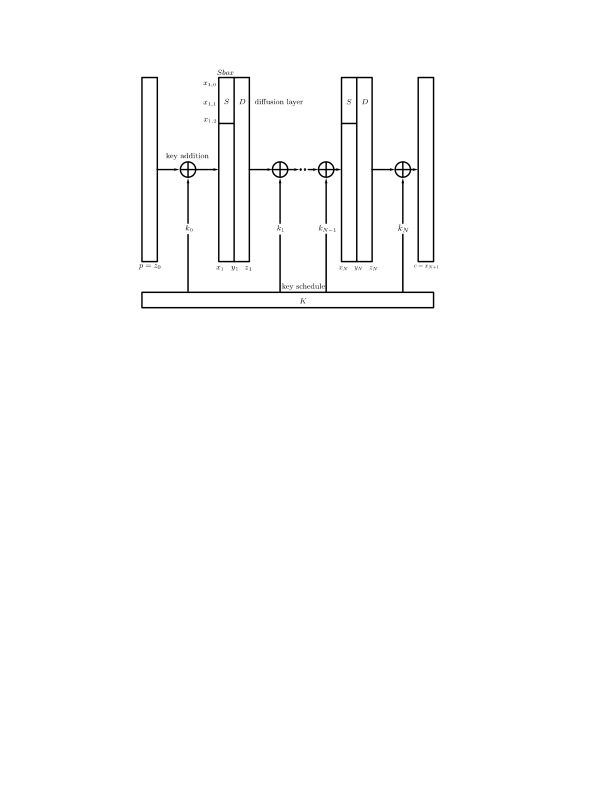
\includegraphics[width=0.7\linewidth]{Images/BlockCipher1}
\caption{ساختار شبکه‌ی جانشینی جایگشتی
	(\lr{SPN})
	در رمزهای قالبی}
\label{fig:blockcipher1}
\end{figure}


تقریباً همه‌ی اجزای شبکه‌های 
\lr{SPN}
به جز جعبه‌های جانشینی را می‌توان با چندجمله‌ای‌های خطی مدل کرد.  جعبه‌های جانشینی را نیز می‌توان به صورت چند‌جمله‌ای‌های درجه دو (مربّعی)
%\LTRfootnote{Quadratic Polynomial}
یا درجات بالاتر، مدل کرد که در بخش‌های بعدی مثال‌هایی از آن را خواهیم دید. بنابراین مدل‌های پایه‌ برای حمله به رمزهای قالبی به شرح زیر است.
\subsubsection*{حمله‌ی جبری متن اصلی معلوم}

در این مدل مهاجم یک یا چند زوج متن اصلی و متن رمزشده‌ را در اختیار دارد و حمله از نوع متن اصلی معلوم و هدف به‌دست آوردن کلید است. برای سادگی فرض کنید طول قالب و طول کلید هر دو برابر 
$n$،
 و تعداد دورها برابر
$N$
باشد و مهاجم فقط یک 
زوج متن اصلی و رمزشده به‌صورت 
$(\textbf{p},\textbf{c})\in \ffld_{2}^{n}\times\ffld_{2}^{n}$
را در اختیار دارد.  او در ابتدا نگاشت‌های چندجمله‌ای متناظر با هر یک از واحدهای بکار رفته در سامانه را به صورت جداگانه به‌دست می‌آورد، سپس با ترکیب این نگاشت‌ها، روابط چندجمله‌ای بین متغیرهای بکار رفته در کل سامانه 
$\Enc_{k}(\cdot)$
را به‌صورت زیر به‌دست می‌آورد. 
\begin{equation*}
\Enc_{k}:\ffld_{2}^{n}\times\ffld_{2}^{n}\ra \ffld_{2}^{n} \Rightarrow\left \{ \begin{array}{ll}
f_{1}(k_{0},...,k_{N},x_{1},\ldots, x_{N+1},y_{1},...,y_{N},z_{0},\ldots, z_{N}) = 0\\
\quad\quad\quad\quad\tab\tab\vdots\\
f_{s}(k_{0},...,k_{N},x_{1},\ldots, x_{N+1} ,y_{1},...,y_{N},z_{0},\ldots, z_{N}) = 0.
\end{array} \right.
\end{equation*}
که در آن
$k_{i}$
نمایش فشرده‌ی بیت‌های کلید در دور 
$i$
است و داریم 
$k_{i} = k_{i0},...,k_{in-1}$.
متغیر 
$x_{i}$
نمایش فشرده بیت‌های وروی به دور 
$i$
ام است و داریم 
$x_{i} = x_{i0},...,x_{in-1}$،
به همین ترتیب متغیر
$y_{i}$
نمایش فشرده‌ی بیت‌های میانی دور 
$i$ام
 و 
$z_{i}$
نمایش فشرده بیت‌های خروجی دور 
$i$ام
 است. تحت نمادگذاری فوق 
$z_{0}$
همان متن اصلی 
$p$
و 
$x_{N+1}$، 
متن رمز شده 
$c$
است. بنابراین مهاجم با جایگذاری مقادیر معلوم 
$\textbf{p}$
و
$\textbf{c}$
در معادلات به‌دست آمده از مرحله‌ی قبل به دستگاه معادلات زیر می‌رسد.

\begin{equation*}
\mS = \left \{ \begin{array}{ll}
f_{1}(k_{0},...,k_{N},x_{1},\ldots, x_{N+1} = \textbf{c},y_{1},...,y_{N},z_{0} = \textbf{p},\ldots, z_{N}) = 0\\
\quad\quad\quad\quad\tab\tab\vdots\\
f_{s}(k_{0},...,k_{N},x_{1},\ldots, x_{N+1} = \textbf{c},y_{1},...,y_{N},z_{0} = \textbf{p},\ldots, z_{N}) = 0.
\end{array} \right.
\end{equation*}


 مجهولات این دستگاه بیت‌های متناظر با متغیرهای میانی و از همه مهم‌تر  بیت‌های کلید است. در اکثر مواقع دستگاه به‌دست آمده جوابی یکتا دارد. بدیهی است که بخشی از جواب متعلق به بیت‌های کلید است و به این ترتیب کلید سامانه به‌دست خواهد آمد. 

برخلاف حملاتی مثل تحلیل تفاضلی یا خطّی که اعمال آن‌ها مشروط به داشتن تعداد زیادی زوج متن اصلی و رمزشده‌آن است، در این نوع حمله‌ معمولاً داشتن فقط یک یا دو زوج متن اصلی و رمزشده آن کافی است تا دستگاه به‌دست آمده یک جواب یکتا داشته باشد و حمله اعمال شود. 

\begin{remark}
	حمله‌  متن اصلی معلوم جبری که در فوق تشریح شد دور از انتظار نیست، تصوّر کنید فرستنده یک فایل با فرمت 
	\lr{pdf}
	%\LTRfootnote{Portable Document Format}
	را بدون هیچ اقدام احتیاطی رمز کرده باشد و مهاجم از این موضوع (نوع فایل)
	مطّلع باشد از آن‌جایی که چهار بایت اول فایل 
	\lr{PDF}
	همواره عبارت است از
	\lr{\%PDF}
	بنابراین مهاجم می‌تواند حمله‌ی فوق را اعمال کند. 
\end{remark}

\begin{remark}
فرآیند جبری سازی و به‌دست آوردن معادلات چندجمله‌ای حاکم بر یک سامانه، می‌تواند یک‌بار انجام شده و سپس به دفعات و در سناریو‌های مختلف مورد استفاده قرار گیرد.
\end{remark}

سناریویی را در نظر بگیرید که چند متن اصلی با یک کلید یکسان رمز شده باشند و مهاجم از این امر مطلع باشد. در این صورت مهاجم ابتدا مانند مرحله‌ی قبل معادلات حاکم بر سامانه را استخراج می‌کند. فرض کنید مهاجم 
$t$
زوج متن اصلی و رمزشده  
$(\textbf{p}_{i},\textbf{c}_{i})$
که همه‌  آن‌ها با یک کلید رمزشده‌اند را در دست دارد. در این صورت با جایگذاری مقادیر معلوم، در معادلات استخراج شده به معادلاتی مانند معادلات زیر دست می‌یابد.
\begin{align*}
\mS = \left \{ \begin{array}{ll}
\mS_{1} = \left \{ \begin{array}{ll}
f_{1}(k_{0},...,k_{N},x_{1}^{1},...,x_{N}^{1}, x_{N+1}^{1} = \textbf{c}_{1} ,y_{1}^{1},...,y_{N}^{1},z_{0}^{1} = \textbf{p}_{1},...,z_{N}^{1}) = 0\\
\quad\quad\tab\tab\vdots\tab\tab\tab\quad\quad\vdots\\
f_{s}(k_{0},...,k_{N},x_{1}^{1},...,x_{N}^{1}, x_{N+1}^{1} = \textbf{c}_{1},y_{1}^{1},...,y_{N}^{1},z_{0}^{1} = \textbf{p}_{1},...,z_{N}^{1}) = 0.
\end{array} \right.
\\
\vdots\\
\mS_{t} = \left \{ \begin{array}{ll}
f_{1}(k_{0},...,k_{N},x_{1}^{t},...,x_{N}^{t}, x_{N+1}^{t} = \textbf{c}_{t},y_{1}^{t},...,y_{N}^{t},z_{0}^{t} = \textbf{p}_{t},...,z_{N}^{t}) = 0\\
\quad\quad\tab\tab\vdots\tab\tab\tab\quad\quad\vdots\\
f_{s}(k_{0},...,k_{N},x_{1}^{t},...,x_{N}^{t}, x_{N+1}^{t} = \textbf{c}_{t},y_{1}^{t},...,y_{N}^{t},z_{0}^{t} = \textbf{p}_{t},...,z_{N}^{t}) = 0.
\end{array} \right.
\end{array} \right.
\end{align*}
نکته‌  قابل توجه در معادلات فوق این است که متغیر متناظر با کلید در همه‌  آن‌ها یکسان است، چرا که 
$t$
متن اصلی با کلیدی یکسان رمز شده‌اند. مهاجم با حل دستگاه معادلات فوق قادر است کلید سامانه را به‌دست آورد. بدیهی است که مهاجم با داشتن تعداد بیشتری متن رمز شده‌  تحت همان کلید، می‌تواند معادلات بیشتری به‌دست آورد که این حل دستگاه را راحت‌تر و در صورت یکتا نبودن جواب (که احتمال آن کم است) تعداد جواب‌هایی را که شامل کلید اصلی نیستند کمتر می‌کند.  در حالتی که مهاجم اطّلاعاتی راجع به متن اصلی ندارد و فقط متن رمز شده را در اختیار دارد حمله ی بعدی را به کار می‌گیرد.
\subsubsection*{حمله‌ی جبری فقط متن رمزشده}
فرض کنید، مهاجم به تعدادی متن رمز‌شده که تحت یک کلید رمز شده‌اند دسترسی دارد.  مانند روش‌های قبل مهاجم می‌تواند دستگاه معادلات چندجمله‌ای  تشکیل دهد که متغیرهای متناظر با کلید در همه معادلات آن مشترک، ولی متغیرهای متناظر با متن اصلی و متغیرهای میانی در آن‌ها متفاوت هستند. پس از آن با جایگذاری متن‌های رمزشده در هر یک از معادلات به‌دست‌آمده به دستگاهی می‌رسد که با حل آن متن اصلی و کلید به‌دست می‌آید. 

\subsection{جبری سازی
	\lr{KeyLoq}}
\subsubsection*{معرفی \en{KeeLoq}}
\en{KeeLoq}، 
یک رمز قالبی با طول قالب متن اصلی و رمزشده ۳۲ بیت و طول کلید ۶۴ بیت است که در سامانه‌های کنترل از راه دور درب خودروها و منازل از آن استفاده می‌شود.  همان‌طور که در شکل 
\ref{fig:keeloq_enc}
نمایش داده شده، بخش اصلی این الگوریتم رمزنگاری از یک ثبات انتقال با بازخورد غیر‌خطی ۳۲ بیتی که تابع بازخورد آن یک تابع غیر خطی ۵ متغیره‌ است تشکیل شده است. علاوه بر این یک ثبات انتقال خطی ۳۲ بیتی دارد که بیت‌های کلید روی آن بارگذاری می‌شوند. 

تابع بازخورد غیرخطی 
$NLF$
در این الگوریتم را با 
\lr{$NLF_{0x3A5C742E}$}، 
نمایش می‌دهیم. این نمایش ضابطه‌ی این تابع را نیز مشخص می‌کند و به این معنی است که، هرگاه معادل ده‌دهی  رشته‌ی باینری ورودی عدد 
$i\in\{0,...,31\}$
باشد، خروجی تابع 
$NLF$
بیت 
$i$ام
از معادل دودویی  عدد هگزادسیمال 
\lr{$0x3A5C742E$}
است. با استفاده از جدول درستی این تابع بولی می‌توان ضابطه‌ی آن را به‌صوررت زیر استخراج کرد. 
\begin{align*}
 &NLF:\ffld_{2}\ra \ffld_{2}\\
 &NLF(a,b,c,d,e) = d + e + ac + ae + bc + be + cd + de + ade + ace + abd + abc.
\end{align*}
\begin{figure}[h]
	\centering
	\includegraphics[width=0.5\linewidth]{Images/keeloq_enc}
	\caption{رمزنگاری در 
		\en{Keeloq}}
	\label{fig:keeloq_enc}
\end{figure}
\renewcommand{\algorithmicrequire}{\textbf{Input:}}
\renewcommand{\algorithmicensure}{\textbf{Output:}}
\begin{algorithm}
	\caption{الگوریتم رمزنگاری  در 
		\en{KeeLoq}}
\label{keeloq enc}
	\begin{latin}
		\begin{algorithmic}[]
			\REQUIRE  $\text{\rl{متن اصلی}}: P = P_{31},...,P_{0}, \text{\rl{کلید}}: \ K = k_{63},...,k_{0}$
			\ENSURE $\text{\rl{متن رمز شده}}: C =C_{31},...,C_{0}$
			\STATE  $X \gets P$ \  \rl{بارگذاری متن اصلی در شیفت رجیستر غیرخطی}
			\FOR{$i = 0,...,527$}			
			\STATE  $OUT \gets NLF(x_{31}, x_{26}, x_{20}, x_{9}, x_{1})$  \ \rl{بیت خروجی تابع غیر خطی}
			\STATE $XOR \gets k_{i \mod 64}\oplus x_{16}\oplus x_{0}\oplus OUT$
			\STATE $\text{\rl{بروزرسانی بیت‌های حالت}}:$
			\begin{enumerate}
				\item
				$X \gets X \ggg 1$ \ \rl{شیفت به راست رجیستر }
				\item 
				$x_{31} \gets XOR$ \ \rl{پر شدن بیت پر ارزش شیفت رجیستر غیر خطی}
			\end{enumerate}
			\ENDFOR
			\RETURN $X$
		\end{algorithmic}
	\end{latin}
\end{algorithm}
فرض کنید بیت‌های متن اصلی را با 
$P_{31},...,P_{0}$، 
و بیت‌های متن رمزشده را با 
$C_{31},...,C_{0}$، 
که 
$P_{0}$
و
$C_{0}$، 
به‌ترتیب بیت‌های کم‌ارزش متن اصلی و متن رمز‌شده هستند، نمایش دهیم. همچنین فرض کنید بیت‌های کلید را با 
$K_{63},...,K_{0}$
که 
$K_{0}$، 
بیت کم‌ارزش کلید است، نمایش دهیم. فرآیند رمزنگاری مطابق  الگوریتم 
\ref{keeloq enc}، 
و به صورت نشان داده شده در شکل 
\ref{fig:keeloq_enc}،
 و 
نحوه رمزگشایی  طبق  الگوریتم 
\ref{keeloq dec}،
و به‌صورت نمایش داده شده در شکل 
\ref{fig:keeloq_dec}
صورت می‌گیرد. 
\begin{figure}[h]
	\centering
	\includegraphics[width=0.5\linewidth]{Images/keeloq_dec}
	\caption{رمزگشایی در 
		\en{Keeloq}}
	\label{fig:keeloq_dec}
\end{figure}
\begin{algorithm}
	\caption{الگوریتم رمزگشایی  در 
		\en{KeeLoq}}
\label{keeloq dec}
	\begin{latin}
		\begin{algorithmic}[]
			\REQUIRE  $\text{\rl{متن رمزشده}}: C = C_{31},...,C_{0}, \text{\rl{کلید}}\ K = k_{63},...,k_{0}$
			\ENSURE $\text{\rl{متن اصلی}}: P =P_{31},...,P_{0}$
			\STATE $Y \gets C$ \ \rl{بارگذاری متن رمز‌شده در شیفت رجیستر غیرخطی}
			\FOR{$i = 0,...,527$}			
			\STATE  $OUT \gets NLF(y_{30}, x_{25}, x_{19}, x_{8}, x_{0})$ \ \rl{بیت خروجی تابع غیر خطی}
			\STATE $ XOR \gets k_{(15 - i) \mod 64}\oplus y_{31}\oplus x_{15}\oplus OUT$
			\STATE \rl{بروزرسانی بیت‌های حالت}
			\begin{enumerate}
				\item
				$Y \gets Y \lll1$ \ \rl{شیفت به چپ رجیستر }
				\item 
				$y_{0} \gets XOR$ \ \rl{پر شدن بیت کم ارزش شیفت رجیستر غیر خطی}
			\end{enumerate}
			\ENDFOR
			\RETURN $X$
		\end{algorithmic}
	\end{latin}
\end{algorithm}
\subsubsection*{روابط بین ورودی و خروجی}
با وجود این‌که  تابع بازخورد 
$NLF$
در کی‌لاک
(\en{Keeloq})
یک چندجمله‌ای از درجه‌ی ۳ است، می‌توان رابطه‌ای چندجمله‌ای با درجه‌ی جبری ۲ بین ورودی و خروجی این  تابع پیدا کرد، که یک نمونه از آن در زیر آمده است.
$$(e + b + a + y)(c + d + y) = 0, $$
که 
$y$
خروجی و 
$a,b,c,d,e$
ورودی تابع بازخورد هستند. در واقع رابطه‌ی چندجمله‌ای فوق رابطه‌ای است که همه‌ی رشته‌های 
$(a,b,c,d,e,y)\in\ffld_{2}^{6}$
که 
$y = NLF(a,b,c,d,e)$
در آن صدق می‌کنند. 

ثبات انتقال  حاوی بیت‌های کلید، در هر دور به اندازه‌ی یک واحد انتقال  چرخشی پیدا می‌کند،  سپس بیت کم ارزش وارد فرآیند رمزنگاری می‌شود. بنابراین اگر بیت‌های کلید مخفی را با 
$k_{31},...,k_{0}$
نمایش دهیم آن‌گاه بیت کلیدی که در دور 
$t$ام
 وارد فرآیند رمزنگاری می‌شود برابر است با 
$k_{(t - 1)\mod 64}$.


فرض کنید بیت‌های حالت اولیه‌  ثبات انتقال با بازخورد غیرخطی  را با 
$L_{31},...,L_{0}$
و بیت‌ حالت تولید شده در دور 
$i$
را با 
$L_{31 + i}$
نمایش  ‌دهیم. در نتیجه آخرین بیت حالتی که تولید می‌شود بیت 
$L_{559}$
متعلق به دور ۵۲۸ام است. با توجه به نمادگذاری فوق رابطه‌  زیر بین متغیر‌های 
$L_{i}$
و بیت‌های متن اصلی و رمزشده برقرار است. 
$$L_{559},...,L_{528} = C_{31},...,C_{0} \ \text{متن رمز شده},$$
$$L_{31},...,L_{0} = P_{31},...,P_{0} \ \text{متن اصلی}.$$

برای یکی‌کردن اندیس‌‌ها در 
$k_{t}$
و
$L_{i}$، 
توجه کنید که بیت حالت 
$L_{i}$
به ازای 
{\small $i\in \{32,...,559\}$}
در دور 
$t = i - 31$
تولید می‌شود. بنابراین بیت کلیدی که برای محاسبه‌ی 
$L_{i}$
به‌کار می‌رود عبارت است از 
{\small $k_{(i - 32)\mod 64}$.}

اکنون می‌توانیم  روابط چندجمله‌ای بین متغیرهای حالت 
$L_{i}$
و متغیرهای 
$k_{i}$
متناظر با بیت‌های کلید را به‌صورت زیر به‌دست آوریم. 
\begin{align*}
\label{keloq eq1}
L_{i} &= P_{i}  \  &\fa i\in \{0,...,31\}\\
L_{i} &= k_{(i - 32)\mod 64} + L_{(i - 32)} + L_{(i - 16)} \ &\fa i\in\{32,...,559\}\\
 \ &+NLF(L_{i-1}, L_{i - 6},L_{i-12},  L_{i - 23}, L_{i - 30}) \ & \\
C_{i - 528} &= L_{i} \ &\fa i\in \{528, 559\}
\end{align*}
با جایگذاری رابطه‌ی درجه‌ی ۳ تابع 
$NLF$
در معادلات فوق به روابط  چندجمله‌ای از درجه‌ی ۳ به‌صورت زیر می‌رسیم. 

{\small \begin{align*}
L_{i} &= P_{i}  \  &\fa i\in \{0,...,31\}\\
L_{i} &= k_{(i - 32)\mod 64} + L_{(i - 32)} + L_{(i - 16)} + L_{i - 23} + L_{i - 30} \ &\fa i\in\{32,...,559\}\\
\ & + L_{i -1}L_{i - 12} + L_{i-1}L_{i - 30} + L_{i - 6}L_{i - 12} + L_{i - 6}L_{i - 30} \ & \\
 \ &+ L_{i - 12}L_{i - 23} + L_{i - 23} L_{i - 30} + L_{i - 1} L_{i - 23} L_{i - 30} \ & \ \\
 \ & +L_{i -1}L_{i - 12}L_{i - 30} + L_{i - 1} L_{i - 6} L_{i - 23} + L_{i -1}L_{i - 6} L_{i - 12} \ &  \ \\
C_{i - 528} &= L_{i} \ &\fa i\in \{528, 559\}
\end{align*}}
اکنون فرض کنید یک زوج متن اصلی و رمزشد‌ه مثل 
$(P,C)$
را داشته باشیم در این صورت با جایگذاری مقادیر 
$L_{i} = P_{i}$
به ازای 
$i\in \{0,...,31\}$
و
$L_{j} = C_{j - 528}$
به ازای 
$j\in\{528,...,559\}$، 
 در روابط فوق،  یک دستگاه معادلات از درجه‌ی ۳ که مجهولات آن بیت‌های کلید و متغیرهای حالت داخلی 
$L_{i}$
به ازای 
$i\in \{32,...,527\}$، 
 هستند به‌دست می‌آید. در نتیجه در مجموع
$560 = 496 + 64$، 
  مجهول و ۵۲۸ معادله‌ی درجه‌ی ۳ خواهیم داشت. اگر فرض کنیم 
$\mu$
تا زوج متن اصلی و رمز شده در دست باشد آن‌گاه به ازای هر زوج، دستگاهی شبیه به دستگاه قبل داریم، که متغیرهای متناظر با بیت‌های کلید در همه‌ی این دستگاه‌ها یکسان است. بنابراین به ازای 
$\mu$
 زوج متن اصلی و رمز شده، دستگاه معادلاتی شامل 
 $496\mu + 64$
 مجهول و 
 $528\mu$
 معادله‌ی درجه‌ی ۳ خواهیم داشت. 
 
می‌توانیم با تغییر متغیر زیر درجه‌ی دستگاه را از 
$3$
 به 
 $2$
  کاهش دهیم.
\begin{align*}
NLF(a,b,c,d,e) =& d + e + ac + \beta + bc + be + cd + de + d\beta + c\beta + \alpha\beta + \alpha c\\
\alpha =& ab\\
\beta =& ae.
\end{align*}
تغییر متغیر فوق سبب می‌شود که هر یک از معادلات قبلی با سه معادله‌ی جدید جایگزین شوند که هر یک از این معادلات، شامل دو متغیر جدید 
$\alpha_{i}$
و
$\beta_{i}$
نیز هستند. دستگاه حاصل در زیر نمایش داده شده. 
{\small \begin{align*}
L_{i} &= P_{i}  \  &\fa i\in \{0,...,31\}\\
L_{i} &= k_{(i - 32)\mod 64} + L_{(i - 32)} + L_{(i - 16)} + L_{i - 23} + L_{i - 30} \ &\fa i\in\{32,...,559\}\\
\ &L_{i -1}L_{i - 12} + \beta_{i} + L_{i - 6}L_{i - 12} + L_{i - 6}L_{i - 30} + L_{i - 12}L_{i - 23}\ & \\
\ &  + L_{i - 23} L_{i - 30} + \beta_{i} L_{i - 23} 
+ \beta_{i}L_{i - 12} + \alpha_{i} L_{i - 23} + \alpha_{i} L_{i - 12} \ &  \ \\
\alpha_{i} &= L_{i-1}L_{i-6} \ &\fa i\in \{32,...,559\}\\
\beta_{i} &= L_{i-1}L_{i-30} \ & \fa i\in \{32,...,559\} \\
C_{i - 528} &= L_{i} \ &\fa i\in \{528,..., 559\}
\end{align*}}
در نتیجه اگر 
$\mu$
زوج متن اصلی و رمز‌شده‌ را داشته باشیم، دستگاهی به‌دست می‌آید که شامل 
$1584\mu$
معادله و 
$1552\mu + 64$
مجهول است. این دستگاه قطعاً دارای جواب خواهد بود چون بطور قطعی از سامانه‌ی رمزنگاری استخراج شده است، ولی ممکن است جواب آن یکتا نباشد. هر چه تعداد زوج متن اصلی و رمز شده‌ای که در اختیار  داریم بیشتر باشد، قیدها یا تعداد معادلات بیشتر شده و جواب به سمت یکتایی پیش می‌رود. برای مثال به ازای 
$\mu = 2$
تعداد معادلات به ۳۱۶۸  (معادله‌ درجه‌ی ۲) و تعداد مجهولات به ۳۱۶۸ می‌رسد.  حل دستگاه به‌دست آمده از این روش با استفاده از روش‌های موجود بسیار دشوار و حتی نشدنی است!  بنابراین صرف جبری سازی یک سامانه‌ی رمزنگاری نمی‌تواند منجر به شکسته شدن آن شود. هدف ما از آوردن این مثال ارائه‌ی یک روش ساده و قابل فهم در تبدیل یک سامانه‌ی رمزنگاری  به دستگاه معادلات چندجمله‌ای بود. روش مذکور تنها روش حمله‌ی جبری به این سامانه‌ی رمزنگاری نیست، برای مشاهده‌ی روش‌های جبری که منجر به شکست عملی 
\en{Keeloq}
شده‌اند، می‌توانید به  
\cite{bard2009algebraic, courtois2008algebraic}
مراجعه کنید. 
\newpage
\subsection{استخراج معادلات جعبه‌های جانشینی}
جعبه‌های جانشینی یکی از بخش‌های کلیدی بسیاری از الگوریتم‌های رمزنگاری نوین، به‌خصوص رمزهای قالبی با معماری شبکه جانشینی-جایگشتی هستند.  جعبه‌ جانشینی در واقع نگاشتی غیرخطی است، که یک 
$m$
بیتی را به یک 
$n$
بیتی می‌نگارد که در این‌صورت آن‌را یک جعبه جانشینی 
$m\times n$
می‌نامند.  در اغلب موارد جعبه‌های جانشینی تنها عامل غیرخطی در ساختار الگوریتم‌های رمزنگاری هستند که  در این بخش قصد داریم روشی برای استخراج معادلات مستقل خطی و با درجه‌ی مشخص برای جعبه‌های جانشینی معرفی کنیم. یکی از روش‌هایی که برای به‌دست آوردن روابط جبری بین متغیرهای ورودی و خروجی یک جعبه جانشیی وجود دارد، به‌دست آوردن تابع بولی هر یک از متغیرهای خروجی بر حسب متغیرهای متناظر با بیت‌های ورودی است. برای مثال جعبه جانشینی 
$3\times 3$، 
با ضابطه 
\begin{center}
	
	\begin{tabular}{|c|c|c|c|c|c|c|c||c|}
		\hline 
		7 & 6 & 5 & 4 & 3 & 2 & 1 & $0$ & $x$ \\ 
		\hline 
		3 & 1 & 5 & 2 & 4 & $0$ & 6 & 7 & $S[x]$ \\ 
		\hline 
	\end{tabular}
	
\end{center}
را در نظر بگیرید. اگر ۳ بیت ورودی را با 
$x_{2},x_{1},x_{0}$، 
و ۳ بیت خروجی را با 
$y_{2},y_{1},y_{0}$، 
که 
$x_{0}$
و 
$y_{0}$، 
به‌ترتیب بیت‌های کم‌ارزش ورودی و خروجی هستند نمایش دهیم آن‌گاه با استفاده از قطعه کد زیر در نرم‌افزار سیج تابع بولی 
$y_{2},y_{1},y_{0}$
را به‌صورت صریح بر حسب متغیرهای 
$x_{2},x_{1},x_{0}$، 
به‌دست می‌آوریم. 
% \begin{latin}
%\begin{flushleft}
%	\begin{lstlisting}
%from sage.crypto.boolean_function import BooleanFunction
%S = mq.SBox(7,6,0,4,2,5,1,3)
%n = S.n
%b = matrix(2^n, n)
%for i in range(2^n):
%    x = bin(i)[2:].zfill(n)
%    b[i] = S(x)
%y2 = BooleanFunction(list(b[:,0])); y2 = y2.algebraic_normal_form()
%y1 = BooleanFunction(list(b[:,1])); y1 = y1.algebraic_normal_form()
%y0 = BooleanFunction(list(b[:,2])); y0 = y0.algebraic_normal_form()
%\end{lstlisting}
%\end{flushleft}
%\end{latin}
 \begin{latin}
\begin{flushleft}
\begin{lstlisting}
S = mq.SBox(7,6,0,4,2,5,1,3)
n = S.n
Y = [0]*n
for i in range(n - 1, -1, -1):
    f = S.component_function(2^i)
    Y[i] = f.algebraic_normal_form()
\end{lstlisting}
\end{flushleft}
\end{latin}
	و در نتیجه داریم	
\begin{align*}
y_{2} =& x_{0} x_{1} + x_{0} x_{2} + x_{1} x_{2} + x_{1} + x_{2} + 1\\
y_{1} =& x_{0} x_{2} + x_{1} + 1\\
y_{0} =& x_{0} x_{1} + x_{0} + x_{1} + x_{2} + 1
\end{align*}
در صورتی که  نگاشت جعبه جانشینی یک‌به‌یک و در نتیجه معکوس‌پذیر باشد، می‌توان تابع بولی هر یک از ورودی‌ها بر حسب خروجی‌ها را نیز به‌دست آورد تا به این‌ترتیب   معادلات بیشتری از جعبه جانشینی داشته باشیم. برای نمونه در مثال قبل می‌توانیم به‌صورت زیر معادلات معکوس را استخراج کنیم. 

 \begin{latin}
\begin{flushleft}
\begin{lstlisting}
m = S.m; n = S.n
P = BooleanPolynomialRing(m + n, ['x' + str(i) for i in range(m)] 
                                               + ['y' + str(i) for i in range(n)])
vars = P.gens()
T = S.inverse()
X = [0]*m
for i in range(m - 1, -1, -1):
	f = T.component_function(2^i)
	f = f.algebraic_normal_form()
	X[i] = f.subs(dict(zip(vars[:m], vars[m:])))
\end{lstlisting}
\end{flushleft}
\end{latin}
 تابع بولی هر یک از ورودی‌ها بر حسب خروجی‌ها، که از اجرای کد فوق به‌دست آمده، به صورت زیر است. 
\begin{align*}
x_{2} =& y_{0} y_{1} + y_{0} + y_{1} y_{2} + y_{1}\\
x_{1} =& y_{0} y_{1} + y_{0} y_{2} + y_{1} + 1\\
x_{0} =& y_{0} y_{1} + y_{2}
\end{align*}
اگر جعبه جانشینی 
$n\times n$، 
معکوس‌پذیر باشد، می‌توانیم با کنار هم قرار دادن معادلات جعبه جانشینی  و معادلات معکوس آن دستگاهی شامل 
$2n$
معادله
و 
$2n$
مجهول برای جعبه جانشینی تشکیل دهیم.   چنان‌چه در 
\cite{cryptoeprint:2017:007}
نیز گزارش شده است، گاهی حل معادلات به‌دست آمده از این روش  سریع‌تر از حل معادلاتی است که  از سایر روش‌ها به‌دست می‌آیند، اما این روش یک محدودیت اساسی دارد و آن درجه بالای جبری توابع بولی است که از این روش به‌دست می‌آید. 

جعبه‌های جانشینی در رمزهای نوین طوری طراحی می‌شنود که درجه توابع بولی  مؤلفه‌ای  آن تا حد امکان بالا باشد تا به این‌ترتیب حل آن‌ها توسط حل‌کننده‌ها سخت‌تر گردد.  به همین دلیل در ادامه روش دیگری را معرفی می‌کنیم که درجه معادلات استخراج شده در آن تا حدی قابل کنترل است. 	 این روش  که در 
\cite{DBLP:conf/fse/BiryukovC03}، 
	معرفی شده و نوع تعمیم‌یافته آن در نرم‌افزار سِیج 
	\gls{SAGE}
	\cite{sagemath}
	 پیاده‌سازی شده است را  روش ماتریس افزوده می‌نامیم، و  با ذکر یک مثال شرح می‌دهیم. 
	 
	 همان جعبه جانشینی قبلی را در نظر بگیرید، این بار  نیز فرض کنید بیت‌های ورودی و خروجی را به ترتیب با 
	$x_{2},x_{1},x_{0}$
	و
	$y_{2},y_{1},y_{0}$، 
	که 
	$x_{0}$
	و 
	$y_{0}$، 
	به‌ترتیب بیت‌های 
	\textit{کم‌ارزش} 
	ورودی و خروجی هستند نمایش دهیم. فرض کنید هدف ما به‌دست آوردن روابط چندجمله‌ای از درجه حداکثر ۲ بین متغیرهای ورودی و خروجی است، برای این‌کار ابتدا یک ماتریس افزوده  به ‌صورت زیر تشکیل می‌دهیم.
	\textbf{\begin{scriptsize} 
			\begin{align*}
			\begin{array}{rrrrrrrrrr}
			0\ & 1 & 2\  & 3 & 4\  & 5 & 6 & 7 & \ \ \ \ \ \ \ \ \ \ \\
			\end{array}\\
			\left(\begin{array}{rrrrrrrrr}
			1 & 1 & 1 & 1 & 1 & 1 & 1 & 1 & 1 \\
			0 & 0 & 0 & 0 & 1 & 1 & 1 & 1 & x_{2} \\
			0 & 0 & 1 & 1 & 0 & 0 & 1 & 1 & x_{1} \\
			0 & 1 & 0 & 1 & 0 & 1 & 0 & 1 & x_{0} \\
			1 & 1 & 0 & 1 & 0 & 1 & 0 & 0 & y_{2} \\
			1 & 1 & 0 & 0 & 1 & 0 & 0 & 1 & y_{1} \\
			1 & 0 & 0 & 0 & 0 & 1 & 1 & 1 & y_{0} \\
			0 & 0 & 0 & 0 & 0 & 0 & 1 & 1 & x_{1} x_{2} \\
			0 & 0 & 0 & 0 & 0 & 1 & 0 & 1 & x_{0} x_{2} \\
			0 & 0 & 0 & 0 & 0 & 1 & 0 & 0 & x_{2} y_{2} \\
			0 & 0 & 0 & 0 & 1 & 0 & 0 & 1 & x_{2} y_{1} \\
			0 & 0 & 0 & 0 & 0 & 1 & 1 & 1 & x_{2} y_{0} \\
			0 & 0 & 0 & 1 & 0 & 0 & 0 & 1 & x_{0} x_{1} \\
			0 & 0 & 0 & 1 & 0 & 0 & 0 & 0 & x_{1} y_{2} \\
			0 & 0 & 0 & 0 & 0 & 0 & 0 & 1 & x_{1} y_{1} \\
			0 & 0 & 0 & 0 & 0 & 0 & 1 & 1 & x_{1} y_{0} \\
			0 & 1 & 0 & 1 & 0 & 1 & 0 & 0 & x_{0} y_{2} \\
			0 & 1 & 0 & 0 & 0 & 0 & 0 & 1 & x_{0} y_{1} \\
			0 & 0 & 0 & 0 & 0 & 1 & 0 & 1 & x_{0} y_{0} \\
			1 & 1 & 0 & 0 & 0 & 0 & 0 & 0 & y_{1} y_{2} \\
			1 & 0 & 0 & 0 & 0 & 1 & 0 & 0 & y_{0} y_{2} \\
			1 & 0 & 0 & 0 & 0 & 0 & 0 & 1 & y_{0} y_{1}
			\end{array}\right)
			\end{align*}
		\end{scriptsize}}
		
		ستون آخر این ماتریس  افزوده،  شامل همه یکجمله‌ای‌های از درجه حداکثر ۲ (به انضمام ۱)  تحت یک ترتیب یکجمله‌ای  است. سایر درایه‌های هر سطر با مقادیری که یکجمله‌ای متناظر با آن سطر به ازای تمام ورودی‌های ممکن، اختیار می‌کند، پر شده‌اند.  
		
		بعد از تشکیل ماتریس،  با عملیات حذفی گاوس ماتریس صفر و یک سمت چپ را به صورت سطری-پلکانی تحویل‌یافته درمی‌آوریم و در طول این فرآیند، هر عملیاتی که روی ماتریس سمت چپ ماتریس افزوده اعمال می‌شود را روی سطرهای ماتریس سمت راست، یعنی ستون شامل یکجمله‌ای‌ها نیز اعمال می‌کنیم که در نتیجه آن ماتریس زیر حاصل می‌شود. 
		\begin{scriptsize}
			\begin{align*}
			\left(\begin{array}{rrrrrrrrr}
			1 & 0 & 0 & 0 & 0 & 0 & 0 & 0 & x_{0} + x_{1} + x_{2} y_{2} + y_{1} + y_{2} + 1 \\
			0 & 1 & 0 & 0 & 0 & 0 & 0 & 0 & x_{1} + x_{2} y_{2} + x_{2} + y_{0} + 1 \\
			0 & 0 & 1 & 0 & 0 & 0 & 0 & 0 & x_{2} y_{2} + x_{2} + y_{2} + 1 \\
			0 & 0 & 0 & 1 & 0 & 0 & 0 & 0 & x_{0} + x_{2} y_{2} + x_{2} + y_{0} + y_{1} \\
			0 & 0 & 0 & 0 & 1 & 0 & 0 & 0 & x_{0} + x_{1} + x_{2} y_{2} + x_{2} + y_{0} + y_{1} + y_{2} + 1 \\
			0 & 0 & 0 & 0 & 0 & 1 & 0 & 0 & x_{2} y_{2} \\
			0 & 0 & 0 & 0 & 0 & 0 & 1 & 0 & x_{0} + x_{2} y_{2} + y_{0} + y_{2} \\
			0 & 0 & 0 & 0 & 0 & 0 & 0 & 1 & x_{1} + x_{2} y_{2} + y_{1} + 1 \\
			0 & 0 & 0 & 0 & 0 & 0 & 0 & 0 & \mathbf{x_{0} x_{2} + x_{1} + y_{1} + 1} \\
			0 & 0 & 0 & 0 & 0 & 0 & 0 & 0 & \mathbf{x_{0} + x_{1} x_{2} + x_{1} + y_{0} + y_{1} + y_{2} + 1} \\
			0 & 0 & 0 & 0 & 0 & 0 & 0 & 0 & \mathbf{x_{0} + x_{2} y_{1} + x_{2} + y_{0} + y_{2}} \\
			0 & 0 & 0 & 0 & 0 & 0 & 0 & 0 & \mathbf{x_{0} + x_{1} + x_{2} y_{0} + x_{2} y_{2} + y_{0} + y_{1} + y_{2} + 1} \\
			0 & 0 & 0 & 0 & 0 & 0 & 0 & 0 & \mathbf{x_{0} x_{1} + x_{0} + x_{1} + x_{2} + y_{0} + 1} \\
			0 & 0 & 0 & 0 & 0 & 0 & 0 & 0 & \mathbf{x_{0} + x_{1} y_{2} + x_{2} y_{2} + x_{2} + y_{0} + y_{1}} \\
			0 & 0 & 0 & 0 & 0 & 0 & 0 & 0 & \mathbf{x_{1} y_{1} + x_{1} + x_{2} y_{2} + y_{1} + 1} \\
			0 & 0 & 0 & 0 & 0 & 0 & 0 & 0 & \mathbf{x_{0} + x_{1} y_{0} + x_{1} + y_{0} + y_{1} + y_{2} + 1} \\
			0 & 0 & 0 & 0 & 0 & 0 & 0 & 0 & \mathbf{x_{0} y_{2} + x_{0} + x_{1} + x_{2} y_{2} + y_{1} + 1} \\
			0 & 0 & 0 & 0 & 0 & 0 & 0 & 0 & \mathbf{x_{0} y_{1} + x_{2} + y_{0} + y_{1}} \\
			0 & 0 & 0 & 0 & 0 & 0 & 0 & 0 & \mathbf{x_{0} y_{0} + x_{1} + y_{1} + 1} \\
			0 & 0 & 0 & 0 & 0 & 0 & 0 & 0 & \mathbf{x_{0} + x_{2} + y_{0} + y_{1} y_{2} + y_{1} + y_{2}} \\
			0 & 0 & 0 & 0 & 0 & 0 & 0 & 0 & \mathbf{x_{0} + x_{1} + y_{0} y_{2} + y_{1} + y_{2} + 1} \\
			0 & 0 & 0 & 0 & 0 & 0 & 0 & 0 & \mathbf{x_{0} + y_{0} y_{1} + y_{2}}
			\end{array}\right)
			\end{align*}
		\end{scriptsize}
		از آن‌جایی که مقدار هر یک از روابط چندجمله‌ای متناظر با سطرهای تمام صفر، به ازای همه‌ی مقادیر ورودی همواره صفر است لذا تمام ورودی و خروجی‌های جعبه جانشینی در معادلاتی که از مساوی صفر قرار دادن این روابط به‌دست می‌آیند صدق می‌کنند. در نتیجه ۱۴ معادله به‌صورت زیر خواهیم داشت.  
{\small \begin{align*}
\begin{split}
0 =& x_{0} x_{2} + x_{1} + y_{1} + 1,\\
0 =& x_{0} + x_{1} x_{2} + x_{1} + y_{0} + y_{1} + y_{2} + 1,\\
0 =& x_{0} + x_{2} y_{1} + x_{2} + y_{0} + y_{2},\\
0 =& x_{0} + x_{1} + x_{2} y_{0} + x_{2} y_{2} + y_{0} + y_{1} + y_{2} + 1,\\
0 =& x_{0} x_{1} + x_{0} + x_{1} + x_{2} + y_{0} + 1,\\
0 =&  x_{0} + x_{1} y_{2} + x_{2} y_{2} + x_{2} + y_{0} + y_{1},\\
0 =&  x_{1} y_{1} + x_{1} + x_{2} y_{2} + y_{1} + 1,\\
\end{split}
\begin{split}
0 =&  x_{0} + x_{1} y_{0} + x_{1} + y_{0} + y_{1} + y_{2} + 1,\\
0 =& x_{0} y_{2} + x_{0} + x_{1} + x_{2} y_{2} + y_{1} + 1,\\
0 =&  x_{0} y_{1} + x_{2} + y_{0} + y_{1},\\
0 =&  x_{0} y_{0} + x_{1} + y_{1} + 1,\\
0 =&  x_{0} + x_{2} + y_{0} + y_{1} y_{2} + y_{1} + y_{2},\\
0 =& x_{0} + x_{1} + y_{0} y_{2} + y_{1} + y_{2} + 1,\\
0 =&  x_{0} + y_{0} y_{1} + y_{2}.
\end{split}
\end{align*}}
با استفاده از دو دستور زیر در نرم‌افزار سِیج،  به‌راحتی می‌توانیم معادلات فوق را استخراج کنیم. 
{\footnotesize \begin{latin}
\begin{flushleft}
\begin{lstlisting}	
S = mq.SBox(7,6,0,4,2,5,1,3)
S.polynomials([x2,x1,x0],[y2,y1,y0])
\end{lstlisting}
\end{flushleft}
\end{latin}}
	
این ۱۴ معادله، مستقل خطی و شامل ۲۲ یکجمله‌ای متمایز هستند. دلیل استقلال خطی این است که هر معادله  شامل یکجمله‌ای‌هایی است که دیگر معادلات فاقد آن هستند.  لازم به‌ذکر است که گاهی ممکن است ماتریس تحویل شده، فاقد سطر تمام‌صفر باشد و در نتیجه نتوانیم معادلات ضمنی درجه دو برای جعبه جانشینی به‌دست آوریم. در این صورت می‌توانیم همین روش را برای به‌دست‌آوردن معادلات درجه 
$3$
و بالاتر تعمیم دهیم.  برای این‌کار کافی است تا ستون آخر ماتریس افزوده را با یکجمله‌ای‌های از درجه  حداکثر 
$3$
(یا بالاتر) پر کنیم  و مانند قبل عمل کنیم.  

یک روش دیگر برای استخراج معادلات جعبه‌های جانشینی استفاده از الگوریتم بوخبرگر مولر است.  یک جعبه جانشینی 
$m\times n$
را در نظر بگیرید، نقاط ورودی و خروجی این جعبه‌جانشینی را می‌توانیم به‌صورت نقاط دودویی از فضای 
$\ffld_{2}^{m + n}$
در نظر بگیریم.  فرض کنید نقاطی  از این فضا که در جعبه جانشینی داده شده‌ صدق می‌کنند  را با 
$V$
نمایش دهیم در این‌صورت اندازه این مجموعه  برابر است با 
$2^{m}$. 
با در نظر گرفتن 
$V$
 به عنوان ورودی الگوریتم بوخبرگر-مولر، خروجی آن چندجمله‌ای‌هایی از  حلقه 
$\ffld_{2}[x_{0}, \ldots, x_{m-1}, y_{0}, \ldots, y_{n-1}]$
خواهند بود که پایه گروبنر 
$I(V)$
را تشکیل می‌دهند.  



\subsection{جبری‌سازی 
	\en{CTC}}
به عنوان یک نمونه دیگر از رمز‌های قالبی، نحوه‌ جبری‌سازی الگوریتم  
\en{CTC}
\LTRfootnote{Courtois Toy Cipher}، 
را بررسی می‌کنیم. این الگوریتم  توسط کورتوا،  در دو نسخه 
\en{CTC1}
\cite{courtois2007fast}، 
و 
\en{CTC2}
\cite{courtois2007ctc2}، 
و فقط برای آزمودن حمله‌های جبری ارائه  شده  است و یک سامانه‌ی رمزنگاری کاربردی محسوب نمی‌شود.  البته  ساختار این  الگوریتم به ساختار بسیاری از الگوریتم‌های رمز قالبی واقعی نظیر  سرپنت 
\LTRfootnote{serpent} 
و
\en{AES}، 
شباهت دارد. این الگوریتم از چند دور  مشابه تشکیل می‌شود. هر دور  شامل سه عملیات اصلی است که عبارتند از، جمع به پیمانه‌ی ۲ با کلید دور، عبور از لایه‌ جعبه‌های جانشینی و سپس عبور بیت‌های خروجی لایه‌ی جعبه‌های جانشینی از یک لایه‌ی انتشار خطی. الگوریتم استخراج کلید هر یک از دورها،  شبیه الگوریتم استخراج کلید در 
\en{DES}
و فقط شامل یک جایگشت ساده روی بیت‌های کلید اصلی (مخفی) است.

پارامترهای اصلی این سامانه عبارتند از 
\begin{enumerate}
	\item 
	جعبه‌های جانشینی یکسان با طول قالب 
	$s = 3$.
	جعبه‌ی جانشینی این سامانه یک نگاشت روی 
	$\ffld_{2^{3}}$
	است که توسط لیست مرتب 
	$[7,6,0,4,2,5,1,3]$
	نیز نمایش داده می‌شود، این نمایش به این معنی است که به ازای ورودی ۳ بیتی 
	$x$
	که معادل  ده‌دهی آن عددی است بین 
	$0$
	تا ۷، خروجی  
	$y$،
	 عضو 
	$x$ام
	 از لیست تعریف شده است. 
	\item 
	تعداد جعبه‌های جانشینی در هر دور، که با 
	$B$
	نمایش داده می‌شود. این پارامتر می‌تواند بین ۱ تا ۱۲۸ متغیر باشد. برای مثال شکل 
	\ref{fig:ctc2}
	یک دور از 
	\en{CTC}
	با 
	$B = 2$
	را نشان می‌دهد. 
	\item 
 طول قالب متن اصلی و  متن رمز شده (بر حسب بیت) برابر 
 $B*s$، 
و طول کلید اصلی برابر است با
$H_{k} = 1,2,3,...$، 
که بیت‌های کلید اصلی را با 
$k = (k_{0},...,k_{H_{k} - 1})$، 
نمایش می‌ دهیم. در 
\en{CTC1}،  
$H_{k} = B*s$، 
اما در 
\en{CTC2}، 
طول قالب الزاما برابر با  
$B*s$
نیست و می‌تواند کوچکتر، مساوی و یا بزرگتر از آن باشد. 
	\item 
	تعداد دورها، که با 
	$N_{r}$
	نمایش داده می‌شود.
	\begin{figure}
		\centering
		\includegraphics[width=0.7\linewidth]{Images/CTC_2}
		\caption{رمز
			\en{CTC}
			با ۲ جعبه‌ی جانشینی در هر دور}
		\label{fig:ctc2}
	\end{figure}
\end{enumerate}

فرض کنید بیت‌های ورودی و خروجی دور 
$i$ام
را به ترتیب با 
$X_{ij}$
و 
$Z_{ij}$
نمایش دهیم که 
$i = 1,...,N_{r}$
و
$j = 1,...,Bs-1$.
با این نحوه‌ی نمایش، 
$Z_{0}$
همان متن اصلی و 
$X_{N_{r}+ 1}$
همان متن رمز شده است که در حمله از نوع  متن اصلی معلوم یا متن رمزی انتخابی  فرض می‌کنیم هر دو معلوم هستند.  در  
\en{CTC1}
کلید هر یک از دورها با یک جایگشت روی بیت‌های کلید اصلی و به‌صورت زیر به‌دست می‌آید. 
$$K_{ij}:= K_{0(j+i\mod Bs)}.$$
که 
$K_{0} = (K_{00},...,K_{0 (B*s - 1)})$
همان کلید اصلی است. 
اما در 
\en{CTC2}
داریم
$$K_{ij} = k_{j + i*509 \ \mod H_{k}}.$$
که 
$k = (k_{0},...,k_{H_{k} - 1})$
کلید اصلی است. \\
به ازای هر دور  
$i = 1,...,Nr$، 
عملکرد لایه‌ی انتشار 
$D$
در 
\en{CTC1}
به صورت 
$$\left\{
\begin{array}{lr}
Z_{i(j*1987 + 257 \mod Bs)} = Y_{i0} &\  \  j = 0\\
Z_{i(j*1987 + 257 \mod Bs)} = Y_{ij}\oplus Y_{i(j+137 \mod Bs)}& \ \fa  \ j\neq 0.\\
\end{array}\right.$$
و در 
\en{CTC2}
به‌صورت زیر است. 
$$\left\{
\begin{array}{lr}
Z_{i(j*1987 + 257 \mod Bs)} = Y_{ij} \oplus Y_{i(j+137 \mod B*s)} \oplus Y_{i(j + 274 \mod B*s)} &\  \  j = 257 \mod B*s\\
Z_{i(j*1987 + 257 \mod Bs)} = Y_{ij}\oplus Y_{i(j+137 \mod Bs)}& \ \text{در غیر این‌صورت}\\
\end{array}\right.$$
که 
$Y_{ij}$
نمایش ورودی لایه‌ی انتشار است. 


شکل 
\ref{fig:ctc10}
یک رمز 
\en{CTC}
با پارامتر
$B = 10$
را نشان می‌دهد. 
\begin{figure}
	\centering
	\includegraphics[width=0.9\linewidth]{Images/CTC_10}
	\caption{رمز 
		\en{CTC}
		با 
		$10$
		جعبه‌ی جانشینی در هر دور}
	\label{fig:ctc10}
\end{figure}
در ادامه نحوه استخراج معادلات حاکم بر یک‌ دور از این الگوریتم را نشان می‌دهیم که به هر تعداد دور دلخواه نیز قابل تعمیم خواهد بود. همان طور که مشاهده شد تنها بخش غیر خطی هر دور از الگوریتم رمزنگاری 
\en{CTC}، 
جعبه‌های جانشینی هستند. معادله‌های حاکم بر دور اول را به‌صورت گام‌به‌گام و در جهت عبور بیت‌های متن اصلی از لایه‌های رمزنگاری به‌دست می‌آوریم.  برای سادگی فرض کنید فقط یک جعبه جانشینی در هر دور به‌کار ببریم. بنابراین پارامترهای 
\en{CTC}، 
در این مثال عبارتند از 
$N_{r} = 1$
و 
$B = 1$.
بیت‌های متن اصلی که عبارتند از 
$(Z_{00},Z_{01},Z_{02})$، 
ابتدا با بیت‌های کلید بر اساس رابطه‌ی 
$X_{i+1j} = Z_{ij}\oplus K_{ij}$، 
به ازای 
$i = 0$
و 
$j = 0, 1, 2$، 
ترکیب می‌شوند، بنابراین سه رابطه به‌صورت زیر خواهیم داشت. 
\begin{align*}
	0 =& K_{00} + Z_{00} + X_{10},\\
	0 =& K_{01} + Z_{01} + X_{11},\\
	0 =& K_{02} + Z_{02} + X_{12}.
\end{align*}
بیت‌ها پس از ترکیب اولیه با کلید اصلی، از لایه‌ جعبه‌های جانشینی عبور می‌کنند. اگر بیت‌های ورودی و خروجی  لایه‌ جعبه‌ جانشینی در دور اول را طبق قرارداد به ترتیب با  
$X_{12},X_{11},X_{10}$ 
و 
$Y_{12}, Y_{11}, Y_{10}$، 
که 
$X_{10}$
و 
$Y_{10}$، 
به‌ترتیب بیت‌های کم‌ارزش ورودی و خروجی هستند نمایش دهیم، آن‌گاه بر اساس روش ماتریس افزوده که در بخش قبل معرفی شد،  ۱۴ رابطه‌ چندجمله‌ای درجه ۲  به‌صورت زیر بین متغیرهای ورودی و خروجی لایه جانشینی به‌دست می‌آید. 
{\small \begin{align*}
\begin{split}
0 =& X_{10} X_{12} + X_{11} + Y_{11} + 1, \\
0 =& X_{10} + X_{11} X_{12} + X_{11} + Y_{10} + Y_{11} + Y_{12} + 1, \\
0 =& X_{10} + X_{12} Y_{11} + X_{12} + Y_{10} + Y_{12},\\
0 =& X_{10} + X_{11} + X_{12} Y_{10} + X_{12} Y_{12} + Y_{10} + Y_{11} + Y_{12} + 1,\\
0 =& X_{10} X_{11} + X_{10} + X_{11} + X_{12} + Y_{10} + 1,\\
0 =& X_{10} + X_{11} Y_{12} + X_{12} Y_{12} + X_{12} + Y_{10} + Y_{11},\\
0 =& X_{11} Y_{11} + X_{11} + X_{12} Y_{12} + Y_{11} + 1,\\
\end{split}
\begin{split}
0 =& X_{10} + X_{11} Y_{10} + X_{11} + Y_{10} + Y_{11} + Y_{12} + 1,\\ 
0 =& X_{10} Y_{12} + X_{10} + X_{11} + X_{12} Y_{12} + Y_{11} + 1,\\
0 =& X_{10} Y_{11} + X_{12} + Y_{10} + Y_{11},\\
0 =& X_{10} Y_{10} + X_{11} + Y_{11} + 1,\\
0 =& X_{10} + X_{12} + Y_{10} + Y_{11} Y_{12} + Y_{11} + Y_{12},\\
0 =& X_{10} + X_{11} + Y_{10} Y_{12} + Y_{11} + Y_{12} + 1,\\
0 =& X_{10} + Y_{10} Y_{11} + Y_{12}.
\end{split}
\end{align*}}
مرحله بعدعبور از لایه انتشار (خطی) است که با استفاده از نحوه‌ی تعریف لایه‌ی خطی 
$D$،
 سه معادله به‌صورت زیر خواهیم داشت. 
{\small \begin{align*}
	0 =& Z_{10} + Y_{11} + Y_{10},\\
	0 =& Z_{11} + Y_{12} + Y_{11},\\
	0 =& Z_{12} + Y_{10}.
\end{align*}}
مرحله‌ی آخر ترکیب بیت‌های خروجی لایه انتشار با بیت‌های کلید دور اول است که سه رابطه‌ زیر را به‌دست می‌دهد. 
{\small \begin{align*}
	0 =& K_{10} + Z_{10} + X_{20},\\
	0 =& K_{11} + Z_{11} + X_{21},\\
	0 =& K_{12} + Z_{12} + X_{22}.
\end{align*}}
در ضمن با توجه به نحوه عمل‌کرد الگوریتم استخراج کلید، روابط زیر بین بیت‌های کلید اصلی و بیت‌های کلید دور اول برقرار است. 
{\small \begin{align*}
	0 =& K_{10} + K_{01},\\
	0 =& K_{11} + K_{02},\\
	0 =& K_{12} + K_{00}.
\end{align*}}
اکنون یک حمله متن رمزی معلوم را در نظر بگیرید، فرض کنید  متن اصلی  
$P = (0, 1, 0)$، 
و متن رمزشده متناظر با آن که برابر است با 
$C = (1, 1, 1)$، 
را در اختیار داشته باشیم و هدف ما به‌دست آوردن کلید باشد.  در این‌صورت با کنار هم قرار دادن معادله‌های هر یک از لایه‌های رمزنگاری و جایگذاری مقادیر متناظر با متن اصلی و رمز شده که به‌ترتیب برابرند با
$(Z_{00},Z_{01},Z_{02}) = (0,1,0)$
و
$(X_{20},X_{21},X_{22}) = (1,1,1)$، 
به دستگاه معادلاتی که در ادامه آمده است می‌رسیم. 
{\small \begin{align*}
\begin{split}
0 =& K_{00} + X_{10},\\
0 =& K_{01} + X_{11} + 1,\\ 
0 =& K_{02} + X_{12},\\
0 =& X_{10} X_{12} + X_{11} + Y_{11} + 1, \\
0 =& X_{10} + X_{11} X_{12} + X_{11} + Y_{10} + Y_{11} + Y_{12} + 1, \\
0 =& X_{10} + X_{12} Y_{11} + X_{12} + Y_{10} + Y_{12},\\
0 =& X_{10} + X_{11} + X_{12} Y_{10} + X_{12} Y_{12} + Y_{10} + Y_{11} + Y_{12} + 1,\\
0 =& X_{10} X_{11} + X_{10} + X_{11} + X_{12} + Y_{10} + 1,\\
0 =& X_{10} + X_{11} Y_{12} + X_{12} Y_{12} + X_{12} + Y_{10} + Y_{11},\\
0 =& X_{11} Y_{11} + X_{11} + X_{12} Y_{12} + Y_{11} + 1,\\
0 =& X_{10} + X_{11} Y_{10} + X_{11} + Y_{10} + Y_{11} + Y_{12} + 1,\\ 
0 =& X_{10} Y_{12} + X_{10} + X_{11} + X_{12} Y_{12} + Y_{11} + 1,\\
0 =& X_{10} Y_{11} + X_{12} + Y_{10} + Y_{11},\\
\end{split}
\begin{split}
0 =& X_{10} Y_{10} + X_{11} + Y_{11} + 1,\\
0 =& X_{10} + X_{12} + Y_{10} + Y_{11} Y_{12} + Y_{11} + Y_{12},\\
0 =& X_{10} + X_{11} + Y_{10} Y_{12} + Y_{11} + Y_{12} + 1,\\
0 =& X_{10} + Y_{10} Y_{11} + Y_{12}\\
0 =& Y_{10} + Z_{12},\\
0 =& Y_{10} + Z_{10} + Y_{11},\\
0 =& Y_{11} + Z_{11} + Y_{12},\\
0 =& K_{10} + Z_{10} + 1,\\
0 =& K_{11} + Z_{11} + 1,\\
0 =& K_{12} + Z_{12} + 1,\\
0 =& K_{01} + K_{10},\\
0 =& K_{02} +K_{11},\\
0 =& K_{00} + K_{12}.
\end{split}
\end{align*}
}
این دستگاه دارای ۲۶ معادله و ۱۵ مجهول و همچنین ۳۱ یکجمله‌ای متمایز است. پایه گروبنر ایده‌ال تولید شده توسط دستگاه معادلات فوق را با استفاده از نرم‌افزار سِیج محاسبه کرده‌ایم که آن‌را در زیر مشاهده می‌کنید. 
{\small $$GB = 
\{K_{00}, K_{01}, K_{02} + 1, Y_{10} + 1, X_{10}, K_{10}, Z_{10} + 1, Y_{11}, X_{11} + 1, K_{11} + 1, Z_{11}, Y_{12}, X_{12} + 1, K_{12}, Z_{12} + 1\}$$}
همان‌طور که مشاهده می‌شود، به‌راحتی می‌توان پاسخ  یکتای دستگاه  را از روی پایه گروبنر محاسبه شده به‌دست آورد. به این ترتیب جواب دستگاه عبارت‌است از
{\small 
$$\{K_{00} = 0, K_{01} = 0, K_{02} = 1, Y_{10} = 1, X_{10} = 0, K_{10} = 0, Z_{10} = 1, Y_{11} = 0, X_{11} = 1, K_{11} = 1,$$
$$Z_{11} = 0, Y_{12} = 0, X_{12} = 1, K_{12} = 0, Z_{12} = 1\}$$
}
و در نتیجه کلید سامانه برابر است با 
$(K_{00},K_{01},K_{02}) = (0,0,1)$. 
 باید توجه کرد که به ازای برخی از زوج متن‌های اصلی و رمز شده ممکن است دستگاهی به‌دست آید که جواب یکتا نداشته باشد، برای مثال اگر متن اصلی 
$P = (0, 0, 0)$ 
را با همان کلید 
$K = (0, 0, 1)$، 
رمز کنیم به متن رمزشده 
$C = (0, 0, 1)$، 
می‌رسیم، حال فرض کنید فقط زوج 
$(P, C)$، 
را در اختیار داشته باشیم. این‌بار دستگاهی که از جایگذاری مقادیر متناظر با 
$P$
و
$C$، 
به‌دست می‌آید، دارای جواب یکتا نیست بلکه ۴ جواب  دارد که بیت‌های کلید در هر چهار جواب، متمایز هستند و لذا برای تشخیص کلید صحیح به زوج متن‌های اصلی و رمزشده بیشتری نیاز داریم.  در فصل بعد راجع به روش‌های حل چنین دستگاه‌هایی بیشتر بحث می‌کنیم. 

\subsection{جبری‌سازی \en{AES}  و  \en{SR}}
\subsubsection*{معرفی \en{AES}}
مؤسسه ملی فناوری و استانداردهای ایالات متحده 
\LTRfootnote{NIST}، 
 با برگزاری یک رقابت چندمرحله‌ای به نام 
 \en{AES}، 
 که از سال ۱۹۹۷ تا سال 
 $2000$
  ادامه داشت،  تلاش کرد تا استاندارد جدیدی برای رمزهای قالبی برگزیند.  الگوریتم پیروز این مسابقه قرار بود استاندارد رمزنگاری  پیشرفته و جایگزین  
  \en{DES}
  باشد. طی یک فراخوان عمومی ۱۵ الگوریتم به مسابقه ارسال شد، از این میان ۵ الگوریتم به مرحله نهایی راه‌یافتند تا این که سرانجام  الگوریتمی تحت عنوان راین‌دال
 \LTRfootnote{Rijndeal}، 
  که توسط دو جوان بلژیکی به نام‌های وینسنت رایمِن
 \LTRfootnote{Vincent Rijmen} 
 و
 یوان دیمِن 
 \LTRfootnote{Joan Daemen}، 
 به مسابقه ارسال شده بود به عنوان برنده مسابقه اعلام شد. الگوریتم راین‌دال پس از پیروزی در مسابقه‌ی 
 \en{AES}،
 توسط 
 \en{NIST}، 
در نوامبر سال 
$2001$
 استانداردسازی و در سند 
\en{FIPS 197}
تحت نام 
\en{AES}
عرضه شد.
\en{AES}، 
مثل بسیاری از رمزهای قالبی دیگر، دارای دو بخش جداگانه است که عبارت‌اند از الگوریتم استخراج کلید و الگوریتم رمزنگاری. الگوریتم رمزنگاری شامل چند دور است که هر دور آن نیازمند کلیدی مختص آن دور و هم‌اندازه با طول قالب است. وظیفه الگوریتم استخراج کلید این است که با دریافت شاه‌کلید اصلی، کلید هر یک از دورها را تولید کند. ما ابتدا فرض می‌کنیم الگوریتم استخراج کلید کار خود را انجام داده و کلید هر یک از دورها را تولید کرده است، با این فرض الگوریتم رمزنگاری را توضیح می‌دهیم و سپس الگوریتم استخراج کلید را توضیح خواهیم داد. 
\en{AES}، 
دارای سه نسخه است که در هرسه، طول قالب داده ثابت و برابر ۱۲۸ بیت، ولی طول کلید و تعداد دورها در این سه نسخه متفاوت، ومطابق جدول  
\ref{tab:AES_Parameters}
 است.
\begin{table}
	\begin{center}
		\begin{tabular}{|c||c|c|c|}
			\hline 
			& طول کلید & طول قالب داده & تعداد دورها \\ 
			\hline 
			\hline
			\lr{AES-128} & ۱۲۸ بیت & ۱۲۸ بیت & $10$ \\ 
			\hline 
			\lr{AES-192} & ۱۹۲ بیت & ۱۲۸ بیت & $12$ \\ 
			\hline 
			\lr{AES-256} & ۲۵۶ بیت & ۱۲۸ بیت & $14$ \\ 
			\hline 
		\end{tabular} 
		\caption{پارامترهای نسخه‌های مختلف \en{AES}}
		\label{tab:AES_Parameters}
	\end{center}
\end{table}
\begin{figure}
	\begin{center}
		%\begin{tikzpicture}[scale=0.7]
%
%\draw (0,3) rectangle node {\scriptsize $0$} +(1,1);
%\draw (0,2) rectangle node {\scriptsize 1} +(1,1);
%\draw (0,1) rectangle node {\scriptsize 2} +(1,1);
%\draw (0,0) rectangle node {\scriptsize 3} +(1,1);
%\draw (1,3) rectangle node {\scriptsize 4} +(1,1);
%\draw (1,2) rectangle node {\scriptsize 5} +(1,1);
%\draw (1,1) rectangle node {\scriptsize 6} +(1,1);
%\draw (1,0) rectangle node {\scriptsize 7} +(1,1);
%\draw (2,3) rectangle node {\scriptsize 8} +(1,1);
%\draw (2,2) rectangle node {\scriptsize 9} +(1,1);
%\draw (2,1) rectangle node {\scriptsize $10$} +(1,1);
%\draw (2,0) rectangle node {\scriptsize 11} +(1,1);
%\draw (3,3) rectangle node {\scriptsize 12} +(1,1);
%\draw (3,2) rectangle node {\scriptsize 13} +(1,1);
%\draw (3,1) rectangle node {\scriptsize 14} +(1,1);
%\draw (3,0) rectangle node {\scriptsize 15} +(1,1);
%
%\end{tikzpicture}
\begin{tikzpicture}
\begin{scope}[xshift = -3.5cm]
\draw[step=0.5cm,color=gray] (-1,-1) grid (1,1);
\edef\a{0}
\foreach \x in {-0.75,-0.25,+0.25,+0.75}
{
	\foreach \y in {+0.75,+0.25,-0.25,-0.75}
	{
		\node at (\x,\y) {$\a$};    
		\pgfmathparse{int(\a+1)};
		\xdef\a{\pgfmathresult}';
	}
}
\end{scope}
\node[] at (-3.5, -1.4)  {\rl{{\footnotesize ماتریس حالت  در 
			\en{AES}}}};
\begin{scope}[xshift = 0cm]
\draw[step=0.5cm,color=gray] (-1,-1) grid (1,1);
\edef\a{0}
\foreach \x in {-0.75,-0.25,+0.25,+0.75}
{
	\foreach \y in {+0.75,+0.25,-0.25,-0.75}
	{
		\node at (\x,\y) {$\a$};    
		\pgfmathparse{int(\a+1)};
		\xdef\a{\pgfmathresult}';
	}
}
\end{scope}
\node[] at (0, -1.4)  {\rl{{\footnotesize آرایش زیرکلید‌ها در 
		\en{AES}}}};
%\begin{scope}[xshift = 3.5cm]
%\draw[step=0.5cm,color=gray] (-1.5,-1) grid (1.5,1);
%\edef\a{0}
%\foreach \x in {-1.25, -0.75, -0.25, +0.25, +0.75, 1.25}
%{
%	\foreach \y in {+0.75, +0.25, -0.25, -0.75}
%	{
%		\node at (\x,\y) {$\a$};    
%		\pgfmathparse{int(\a+1)};
%		\xdef\a{\pgfmathresult}';
%	}
%}
%\end{scope}
%\node[] at (3.5, -1.4)  {\rl{{\footnotesize آرایش کلید در 
%			\en{AES-192}}}};
%\begin{scope}[xshift = 7.5cm]
%\draw[step=0.5cm,color=gray] (-1.5,-1) grid (2.5,1);
%\edef\a{0}
%\foreach \x in {-1.25, -0.75, -0.25, +0.25, +0.75, 1.25, 1.75, 2.25}
%{
%	\foreach \y in {+0.75, +0.25, -0.25, -0.75}
%	{
%		\node at (\x,\y) {$\a$};    
%		\pgfmathparse{int(\a+1)};
%		\xdef\a{\pgfmathresult}';
%	}
%}
%\end{scope}
%\node[] at (8, -1.4)  {\rl{{\footnotesize آرایش کلید در 
%			\en{AES-256}}}};
\end{tikzpicture}%
		\caption{آرایش داده و کلید در   \en{AES}}
		\label{fig:data_array_AES}
	\end{center}
\end{figure}
در ادامه خواهیم دید، برخلاف این‌که طول کلید در نسخه‌های مختلف 
\en{AES}
متفاوت است ولی،  هر یک از زیرکلیدها یا کلید دورها که توسط الگوریتم استخراج کلید تولید می‌شوند هم‌طول با قالب داده یعنی ۱۲۸ بیتی هستند. برای شرح عمل‌کرد  
\en{AES}، 
قالب داده و زیرکلید‌ها را به صورت آرایه‌های 
$4\times 4$
از کلمه‌های یک بایتی و با آرایش نشان داده شده در شکل 
\ref{fig:data_array_AES}
در نظر می‌گیریم و ماتریس  شامل داده در حال رمزنگاری را ماتریس حالت 
می‌نامیم. 

بین مجموعه‌ی بایت‌ها و میدان 
$\gf(2^{8})$
تناظری یک‌به‌یک به‌صورت زیر برقرار است. 
\begin{align*}
\ffld_{2}^{8}\ra \gf(2^{8}) &= \frac{\gf(2)[X]}{\langle X^{8} + X^{4} + X^{3} + X + 1\rangle} = \gf(2)(\theta)\\
(b_{7},...,b_{0})&\mapsto \sum_{i = 0}^{7}b_{i}X^{i}\mod m(X) = \sum_{i = 0}^{7}b_{i}\theta^{i}
\end{align*}
که 
$m(X) = X^{8} + X^{4} + X^{3} + X + 1\in \gf(2)[X]$
یک چندجمله‌ای تحویل‌ناپذیر از حلقه 
$\gf(2)[X]$، 
 موسوم به چندجمله‌ای راین‌دال، و 
 $\theta$
 یک ریشه آن است.  با استفاده از این تناظر می‌توانیم هر  بایت را به صورت یک چندجمله‌ای از میدان 
 $\gf(2)(\theta)$
  در نظر بگیریم، برای مثال 
$\texttt{0xD1} = \theta^{7} + \theta^{6} + \theta^{4} + 1$. 
  به این ترتیب  ماتریس حالت، عضوی از فضای 
$\mat_{4}(\ffld_{2^{8}})$
 است.  به همین ترتیب کلید هر یک از دورها را نیز می‌توانیم به‌صورت یک ماتریس از 
$\mat_{4}(\ffld_{2^{8}})$
در نظر بگیریم. در ادامه با استفاده از این تناظر، یک بیان جبری از سامانه رمزنگاری 
\en{AES}
ارائه خواهیم کرد. فرض کنید تعداد دورها را با 
$n$
نمایش دهیم. در این‌صورت فرآیند رمزنگاری مطابق الگوریتم 
\ref{alg:AES_enc}
است. 
\begin{algorithm}
	\caption{الگوریتم رمزنگاری  
		\en{AES}}
		\label{alg:AES_enc}	
	\begin{latin}
		\begin{algorithmic}[]
			\REQUIRE  $P\in \mat_{4}(\ffld_{2^{8}})$ \ \rl{متن اصلی}
			\REQUIRE $K_{0},...,K_{n}\in \mat_{4}(\ffld_{2^{8}})$ \ \rl{{\small کلید‌های هر یک از دورها که توسط الگوریتم استخراج کلید تولید شده‌اند}}
			\ENSURE $C \in \mat_{4}(\ffld_{2^{8}})$
			\STATE $S_{0}\gets \texttt{AddRoundKey}(P, K_{0})$ \ \rl{سفیدسازی}
			\FOR{$r = 1,...,n$}		
			\STATE $S_{r}\gets \texttt{SubByte}(S_{r-1})$
			\STATE $S_{r}\gets \texttt{ShiftRows}(S_{r})$
			\IF{ $r \neq N_{r}$}
			\STATE{$S_{r} \gets \texttt{MixColumns}(S_{r})$}
			\ENDIF
			\STATE{$S_{r} \gets \texttt{AddRoundKey}(S_{r}, K_{r})$}
			\ENDFOR
			\STATE $C \gets S_{n}$
			\RETURN $C$
		\end{algorithmic}
	\end{latin}
\end{algorithm}
همان‌طور که در شکل 
\ref{fig:AES_RoundFunction}
نیز نمایش داده شده، هر دور از حلقه اصلی  الگوریتم 
\ref{alg:AES_enc}، 
(به استثنا دور آخر) شامل ۴  عملیات مختلف است که در ادامه هر یک را توضیح می‌دهیم. 
\begin{figure}[h]
\begin{center}
\begin{tikzpicture}[scale=0.5]

%\draw[thick, dashed,] (-1,-2) rectangle (29,7) node[above left] {\rl{تابع دور در 
%		\en{AES}}};
\draw[thick,->] (-3,2) -- ++(3,0);
\draw[thick,->] (28,2) -- ++(3,0);

\defineStateSize{4}
\defineArrowLength{2}
\defineTextSize{0.4cm}
\defineTextArrowSize{0.3cm}
\defineXGap{0}
\defineYGap{5}
\defineStateIndex{0}
\defineLinkRound{1}
\initdiffpath

%\colorstate{
%	....
%	....
%	....
%	....
%}{AK}

\colorstate{
	....
	....
	....
	....
}{SB}

\draw[->, thick,shift={(1,-0.5)}] (0.5, 4) 
-- ++(0, 1.5) 
-- node[above] {\textsf{SubByte}} ++(6, 0) -- ++(0, -1.5);

\colorstate{
	...x
	...x
	...x
	...x
}{SR}

\fill[color=lightgray] (15,0) rectangle ++(1,4);
\fill[color=lightgray] (21,0) rectangle ++(1,4);
\draw[->, thick,shift={(15,0)}] (0.5, 4) 
-- ++(0, 1) 
-- node[above] {$C\gets \mathbf{Mix}\times C$} ++(6, 0) 
-- ++(0, -1);

\colorstate{
	...x
	..x.
	.x..
	x...
}{MC}
\colorstate{
	....
	....
	....
	....
}{AK}
\colorstate{
	....
	....
	....
	....
}{0}
\path ( 2,-1) node {{\scriptsize $S_{r-1}$}};
\path ( 8,-1) node {{\scriptsize $S_{r} = \texttt{ShiftRows}(S_{r-1})$}};
\path (14,-1) node {{\scriptsize $\texttt{SubBytes}(S_{r})$}};
\path (20,-1) node {{\scriptsize $\texttt{MixColumns}(S_{r})$}};
\path (26,-1) node {{\scriptsize $\texttt{AddRoundKey}(S_{r})$}};
\end{tikzpicture}
\caption{نمایش تصویری یک دور از الگوریتم 
	\en{AES}}
\label{fig:AES_RoundFunction}
\end{center}
\end{figure}
\paragraph*{\texttt{AddRoundKey}}
در این تابع ماتریس حالت با کلید دور ترکیب می‌شود، به‌این‌صورت که هر بایت از ماتریس ورودی با بایت متناظر از کلید دور،
\texttt{xor}
می‌شود، و یا به بیان جبری، ماتریس حالت و ماتریس کلید به عنوان دو ماتریس از فضای 
$\mat_{4}(\ffld_{2^{8}})$
با هم جمع می‌شوند. 

قبل از توضیح مرحله بعد دو مفهوم جبری را تعریف می‌کنیم. در تعاریف زیر فرض کنید 
$\ffld$
یک میدان از مرتبه 
$q$
و 
$\fld$
یک توسیع 
$\ffld$
از درجه 
$d$
باشد. 
\begin{definition}[\textbf{مزدوج‌های یک عضو میدان}]
فرض کنید 
$a\in\fld$، 
در این‌صورت مزوج‌های 
$a$
نسبت به 
$\ffld$
عبارت‌اند از اعضای مجموعه 
$\{a^{q^{i}}: \ 0\leq i\leq d-1\}$.
\end{definition}
\begin{definition}[\textbf{$q$-
	چندجمله‌ای}]
چندجمله‌ای 
$f(x) = \sum_{i = 0}^{d-1}a_{i}x^{q^{i}}\in\fld[x]$ 
را که 
$a_{i}\in \fld$، 
یک 
$q$-
چندجمله‌ای گوییم. بنابراین وقتی 
$f(x)$
یک 
$q$-
چندجمله‌ای باشد، آن‌گاه به ازای هر 
$a\in \fld$
مقدار 
$f(a)$
ترکیب 
$\fld$-
خطی از مزدوج‌های 
$a$
خواهد بود. 
\end{definition}
یک 
$q$
-چندجمله‌ای مثل 
$f(x)\in\fld[x]$
یک نگاشت خطی روی 
$\fld$
به عنوان فضای برداری  روی 
$\ffld$ 
است. همچنین می‌توان نشان داد که هر نگاشت خطی روی 
$\fld$ 
به عنوان یک فضای برداری روی 
$\ffld$
را می‌توان به‌صورت یک 
$q$
-چندجمله‌ای بیان کرد. برای مثال هر نگاشت خطی روی 
$\gf(2^{8})$
به عنوان یک فضای برداری روی 
$\gf(2)$
را می‌توان به‌صورت 
$f(X) = \lambda_{0}X^{2^{0}} + \lambda_{1}X^{2^{1}} + \ldots + \lambda_{7}X^{2^{7}}$
 نوشت که در آن 
 $\lambda_{i}\in \gf(2^{8})$.
\paragraph*{\texttt{SubByte}}
در این مرحله  هر بایت از ماتریس ورودی از جعبه جانشینی 
\en{AES} 
عبور کرده و بایت متناظر در ماتریس خروجی را تشکیل می‌دهد. جعبه جانشینی شامل سه عملیات مختلف است که آن‌ها را توضیح می‌دهیم. 
\begin{itemize}
\item[-]
اولین عملیات جعبه جانشینی معکوس‌گیری توسیع یافته است. به این‌خاطر آن‌را توسیع یافته گوییم که صفر نیز عضو دامنه این نگاشت است و طبق قرارداد آن‌را به‌خودش می‌نگارد. با توجه به این‌که مرتبه میدان 
$\gf(2^{8})$
برابر 
$256$
است لذا به ازای هر 
$w\in\gf(2^{8})\backslash \{0\}$
داریم 
$w^{-1} = w^{254}$. 
همچنین 
$0^{254}  = 0$
بنابراین می‌توان این مرحله را با استفاده از نگاشت زیر توصیف کرد. 
\begin{align*}
I:\gf(2^{8})&\ra \gf(2^{8})\\
w = \sum_{i = 0}^{7} w_{i}\theta^{i}&\mapsto x = I(w) = w^{254}.
\end{align*}
\item[-]
گام دوم اِعمال یک نگاشت 
$\gf(2)$
-خطی به‌صورت زیر است. 
$$
x = \begin{pmatrix}
x_{0}\\
x_{1}\\
x_{2}\\
x_{3}\\
x_{4}\\
x_{5}\\
x_{6}\\
x_{7}\\
\end{pmatrix} \mapsto
\begin{pmatrix}
1&0&0&0&1&1&1&1\\
1&1&0&0&0&1&1&1\\
1&1&1&0&0&0&1&1\\
1&1&1&1&0&0&0&1\\
1&1&1&1&1&0&0&0\\
0&1&1&1&1&1&0&0\\
0&0&1&1&1&1&1&0\\
0&0&0&1&1&1&1&1
\end{pmatrix}
\begin{pmatrix}
x_{0}\\
x_{1}\\
x_{2}\\
x_{3}\\
x_{4}\\
x_{5}\\
x_{6}\\
x_{7}\\
\end{pmatrix}
$$
می‌دانیم که هر نگاشت خطی روی 
$\gf(2^{8})$
به عنوان یک فضای برداری روی 
$\gf(2)$
را می‌توان به‌صورت یک 
$2$
-چندجمله‌ای نوشت. 
$2$
-چندجمله‌ای متناظر با نگاشت خطی فوق عبارت‌است از 
$$x \mapsto A(x) = \texttt{05}x^{2^{0}} + \texttt{09}x^{2^{1}} + \texttt{F9}x^{2^{2}} + \texttt{25}x^{2^{3}} + \texttt{F4}x^{2^{4}} + \texttt{01}x^{2^{5}} + \texttt{B5}x^{2^{6}} + \texttt{8F}x^{2^{7}}$$
\item[-]
گام آخر در جعبه جانشینی افزودن مقدار ثابت است. در این مرحله خروجی گام دوم و مقدار ثابت 
$\texttt{63} = \theta^{6} + \theta^{5} + \theta + 1\in \gf(2^{8})$
به عنوان اعضای میدان 
$\gf(2^{8})$
با هم جمع می‌شوند و حاصل خروجی جعبه جانشینی خواهد بود. 
\end{itemize}
بنابراین اگر نگاشت جعبه جانشینی را با 
$S_{RD}:\gf(2^{8})\ra\gf(2^{8})$
نمایش دهیم در این‌صورت داریم 
$S_{RD}(w) = A(I(w)) + \texttt{63}$.
\paragraph*{\texttt{ShiftRows}}
همان‌طور که در شکل 
\ref{fig:AES_RoundFunction}
نمایش داده شده،  در این مرحله کلمه‌های  سطر 
$i$ام 
از آرایه داده به اندازه 
$0\leq i\leq 3$
به سمت چپ انتقال چرخشی پیدا می‌کنند. همان‌طور که مشخص است این مرحله مستقل از تعداد سطرها است و سطر اول در این مرحله بدون تغییر باقی می‌ماند.اگر این انتقال  چرخشی سطرها  وجود نداشته باشد، کل عملیات رمزنگاری روی ستون‌های ۳۲ بیتی انجام می‌شود، و ما در عمل یک رمز قالبی با طول قالب ۳۲ بیت خواهیم داشت!
\paragraph*{\texttt{MixColumns}}
این تابع هر ستون از ماتریس حالت را به‌طور مستقل از دیگر ستون‌ها تلفیق و درهم‌سازی می‌کند. فرآیند تلفیق بدین ترتیب است که هر ستون از ماتریس حالت، در  ماتریس ثابت 
\begin{equation*}
\begin{pmatrix}
\theta&\theta+1&1&1\\
1&\theta&\theta + 1&1\\
1&1&\theta&\theta + 1\\
\theta + 1&1&1&\theta
\end{pmatrix} = 
\begin{pmatrix}
	\texttt{02}&\texttt{03}&\texttt{01}&\texttt{01}\\
	\texttt{01}&\texttt{02}&\texttt{03}&\texttt{01}\\
	\texttt{01}&\texttt{01}&\texttt{02}&\texttt{03}\\
	\texttt{03}&\texttt{01}&\texttt{01}&\texttt{02}
\end{pmatrix}\in
\mM_{4}(\ffld_{2^{8}})
\end{equation*}
ضرب می‌شود تا ستون جدید متناظر، در ماتریس حالت خروجی به‌دست آید.


الگوریتم توسیع یا استخراج کلید وابسته به طول کلید،  متفاوت است. در این میان الگوریتم توسیع کلید 
\en{AES-256}
دارای یک تفاوت جزیی نسبت به دو نسخه دیگر است. ما برای سادگی، فقط الگوریتم توسیع کلید نسخه‌های 
\en{AES-128}
و 
\en{AES-192}
را  شرح می‌دهیم.   کلید هر دور بر اساس کلید دور قبل و به‌صورت نمایش داده شده در شکل 
\ref{fig:AES_keyschedule}
 به‌دست می‌آید. 
\begin{figure}[h]
\begin{center}
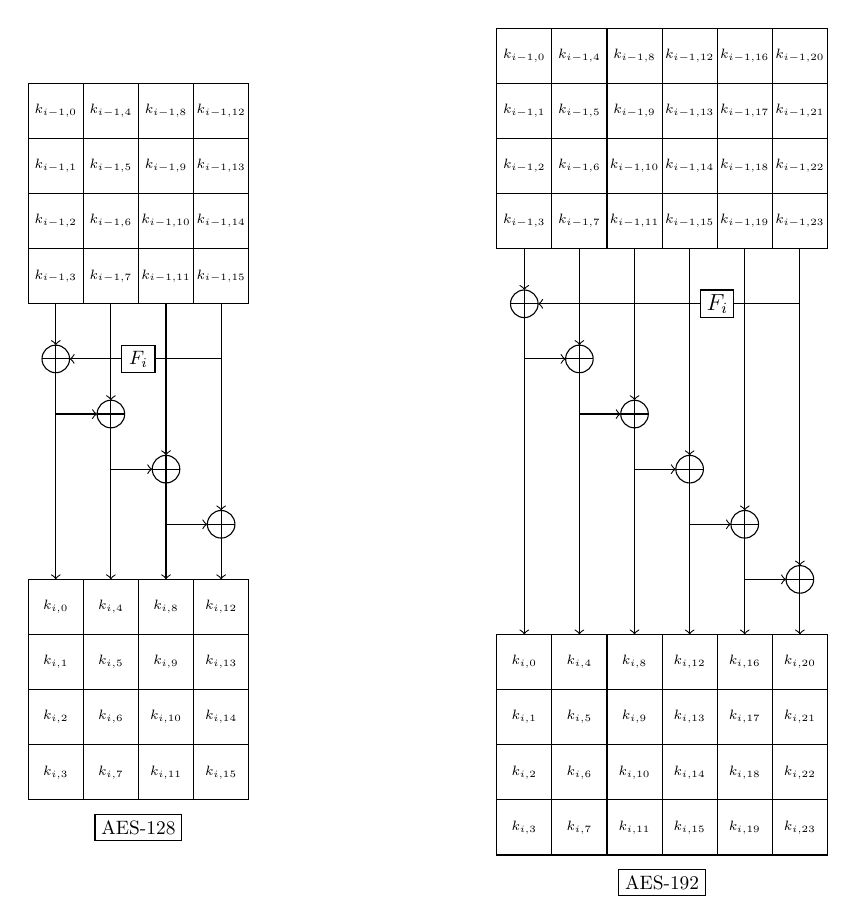
\begin{tikzpicture}[scale=0.7]

\tikzstyle{every node}=[transform shape];
\begin{scope}[xshift=-4cm, shift={(-0.5,-1)}]
\begin{scope}[xshift=0cm]
\draw (0,3) rectangle node {\scriptsize $k_{i-1,0}$} +(1,1);
\draw (0,2) rectangle node {\scriptsize $k_{i-1,1}$} +(1,1);
\draw (0,1) rectangle node {\scriptsize $k_{i-1,2}$} +(1,1);
\draw (0,0) rectangle node {\scriptsize $k_{i-1,3}$} +(1,1);
\draw (1,3) rectangle node {\scriptsize $k_{i-1,4}$} +(1,1);
\draw (1,2) rectangle node {\scriptsize $k_{i-1,5}$} +(1,1);
\draw (1,1) rectangle node {\scriptsize $k_{i-1,6}$} +(1,1);
\draw (1,0) rectangle node {\scriptsize $k_{i-1,7}$} +(1,1);
\draw (2,3) rectangle node {\scriptsize $k_{i-1,8}$} +(1,1);
\draw (2,2) rectangle node {\scriptsize $k_{i-1,9}$} +(1,1);
\draw (2,1) rectangle node {\scriptsize $k_{i-1,10}$} +(1,1);
\draw (2,0) rectangle node {\scriptsize $k_{i-1,11}$} +(1,1);
\draw (3,3) rectangle node {\scriptsize $k_{i-1,12}$} +(1,1);
\draw (3,2) rectangle node {\scriptsize $k_{i-1,13}$} +(1,1);
\draw (3,1) rectangle node {\scriptsize $k_{i-1,14}$} +(1,1);
\draw (3,0) rectangle node {\scriptsize $k_{i-1,15}$} +(1,1);
\end{scope}

\begin{scope}[yshift=-9cm]
\draw (0,3) rectangle node {\scriptsize $k_{i,0}$} +(1,1);
\draw (0,2) rectangle node {\scriptsize $k_{i,1}$} +(1,1);
\draw (0,1) rectangle node {\scriptsize $k_{i,2}$} +(1,1);
\draw (0,0) rectangle node {\scriptsize $k_{i,3}$} +(1,1);
\draw (1,3) rectangle node {\scriptsize $k_{i,4}$} +(1,1);
\draw (1,2) rectangle node {\scriptsize $k_{i,5}$} +(1,1);
\draw (1,1) rectangle node {\scriptsize $k_{i,6}$} +(1,1);
\draw (1,0) rectangle node {\scriptsize $k_{i,7}$} +(1,1);
\draw (2,3) rectangle node {\scriptsize $k_{i,8}$} +(1,1);
\draw (2,2) rectangle node {\scriptsize $k_{i,9}$} +(1,1);
\draw (2,1) rectangle node {\scriptsize $k_{i,10}$} +(1,1);
\draw (2,0) rectangle node {\scriptsize $k_{i,11}$} +(1,1);
\draw (3,3) rectangle node {\scriptsize $k_{i,12}$} +(1,1);
\draw (3,2) rectangle node {\scriptsize $k_{i,13}$} +(1,1);
\draw (3,1) rectangle node {\scriptsize $k_{i,14}$} +(1,1);
\draw (3,0) rectangle node {\scriptsize $k_{i,15}$} +(1,1);
\end{scope}

\draw[->] (0.5,0) -- ++(0,-1+0.25);
\draw[] (0.5,-1) circle (0.25);
\draw[] (0.25,-1) -- ++(0.5,0);  
\draw[->] (3.5,-1) -- ++(-3+0.25,0);
%\draw[fill=white] (2.5+0.2,-1-0.25) rectangle node{\large\texttt{<<<}} ++(1-0.4,0.5);
\draw[fill=white] (1.5+0.2,-1-0.25) rectangle node {\textsf{$F_{i}$}} ++(1-0.4,0.5);
\draw[->] (0.5,-1+0.25) --  ++(0,-4.5+0.25);

\draw[->] (1.5,0) -- ++(0,-2+0.25);
\draw[->] (1.5,-2+0.25) -- ++(0,-3.25);
\draw[->] (0.5,-2) -- ++(1-0.25,0);
\draw[]   (1.5,-2) circle (0.25);
\draw[]   (1.25,-2) -- ++(0.5,0);  

\draw[->] (2.5,0) -- ++(0,-3+0.25);
\draw[->] (2.5,-3+0.25) -- ++(0,-2.25);
\draw[->] (1.5,-3) -- ++(1-0.25,0);
\draw[]   (2.5,-3) circle (0.25);
\draw[]   (2.25,-3) -- ++(0.5,0);  

\draw[->] (3.5,0) -- ++(0,-4+0.25);
\draw[->] (3.5,-4+0.25) -- ++(0,-1.25);
\draw[->] (2.5,-4) -- ++(1-0.25,0);
\draw[]   (3.5,-4) circle (0.25);
\draw[]   (3.25,-4) -- ++(0.5,0);  
\end{scope}
\node[draw] at (-2.5,-10.5) {AES-128};

\begin{scope}[xshift = 4cm]
\begin{scope}[xshift=0cm]
\draw (0,3) rectangle node {\scriptsize $k_{i-1,0}$} +(1,1);
\draw (0,2) rectangle node {\scriptsize $k_{i-1,1}$} +(1,1);
\draw (0,1) rectangle node {\scriptsize $k_{i-1,2}$} +(1,1);
\draw (0,0) rectangle node {\scriptsize $k_{i-1,3}$} +(1,1);
\draw (1,3) rectangle node {\scriptsize $k_{i-1,4}$} +(1,1);
\draw (1,2) rectangle node {\scriptsize$k_{i-1,5}$} +(1,1);
\draw (1,1) rectangle node {\scriptsize$k_{i-1,6}$} +(1,1);
\draw (1,0) rectangle node {\scriptsize$k_{i-1,7}$} +(1,1);
\draw (2,3) rectangle node {\scriptsize$k_{i-1,8}$} +(1,1);
\draw (2,2) rectangle node {\scriptsize$k_{i-1,9}$} +(1,1);
\draw (2,1) rectangle node {\scriptsize$k_{i-1,10}$} +(1,1);
\draw (2,0) rectangle node {\scriptsize$k_{i-1,11}$} +(1,1);
\draw (3,3) rectangle node {\scriptsize$k_{i-1,12}$} +(1,1);
\draw (3,2) rectangle node {\scriptsize$k_{i-1,13}$} +(1,1);
\draw (3,1) rectangle node {\scriptsize$k_{i-1,14}$} +(1,1);
\draw (3,0) rectangle node {\scriptsize$k_{i-1,15}$} +(1,1);
\draw (4,3) rectangle node {\scriptsize$k_{i-1,16}$} +(1,1);
\draw (4,2) rectangle node {\scriptsize$k_{i-1,17}$} +(1,1);
\draw (4,1) rectangle node {\scriptsize$k_{i-1,18}$} +(1,1);
\draw (4,0) rectangle node {\scriptsize$k_{i-1,19}$} +(1,1);
\draw (5,3) rectangle node {\scriptsize$k_{i-1,20}$} +(1,1);
\draw (5,2) rectangle node {\scriptsize$k_{i-1,21}$} +(1,1);
\draw (5,1) rectangle node {\scriptsize$k_{i-1,22}$} +(1,1);
\draw (5,0) rectangle node {\scriptsize$k_{i-1,23}$} +(1,1);
\end{scope}

\begin{scope}[yshift=-11cm]
\draw (0,3) rectangle node {\scriptsize $k_{i,0}$} +(1,1);
\draw (0,2) rectangle node {\scriptsize$k_{i,1}$} +(1,1);
\draw (0,1) rectangle node {\scriptsize$k_{i,2}$} +(1,1);
\draw (0,0) rectangle node {\scriptsize$k_{i,3}$} +(1,1);
\draw (1,3) rectangle node {\scriptsize$k_{i,4}$} +(1,1);
\draw (1,2) rectangle node {\scriptsize$k_{i,5}$} +(1,1);
\draw (1,1) rectangle node {\scriptsize$k_{i,6}$} +(1,1);
\draw (1,0) rectangle node {\scriptsize$k_{i,7}$} +(1,1);
\draw (2,3) rectangle node {\scriptsize$k_{i,8}$} +(1,1);
\draw (2,2) rectangle node {\scriptsize$k_{i,9}$} +(1,1);
\draw (2,1) rectangle node {\scriptsize$k_{i,10}$} +(1,1);
\draw (2,0) rectangle node {\scriptsize$k_{i,11}$} +(1,1);
\draw (3,3) rectangle node {\scriptsize$k_{i,12}$} +(1,1);
\draw (3,2) rectangle node {\scriptsize$k_{i,13}$} +(1,1);
\draw (3,1) rectangle node {\scriptsize$k_{i,14}$} +(1,1);
\draw (3,0) rectangle node {\scriptsize$k_{i,15}$} +(1,1);
\draw (4,3) rectangle node {\scriptsize$k_{i,16}$} +(1,1);
\draw (4,2) rectangle node {\scriptsize$k_{i,17}$} +(1,1);
\draw (4,1) rectangle node {\scriptsize$k_{i,18}$} +(1,1);
\draw (4,0) rectangle node {\scriptsize$k_{i,19}$} +(1,1);
\draw (5,3) rectangle node {\scriptsize$k_{i,20}$} +(1,1);
\draw (5,2) rectangle node {\scriptsize$k_{i,21}$} +(1,1);
\draw (5,1) rectangle node {\scriptsize$k_{i,22}$} +(1,1);
\draw (5,0) rectangle node {\scriptsize$k_{i,23}$} +(1,1);
\end{scope}

\draw[->] (0.5,0) -- ++(0,-1+0.25);
\draw[] (0.5,-1) circle (0.25);
\draw[] (0.25,-1) -- ++(0.5,0);  
\draw[->] (5.5,-1) -- ++(-5+0.25,0);
%\draw[fill=white] (4.5+0.2,-1-0.25) rectangle node{\large\texttt{<<}} ++(1-0.4,0.5);
\draw[fill=white] (3.5+0.2,-1-0.25) rectangle node{\large\textsf{$F_{i}$}} ++(1-0.4,0.5);
\draw[->] (0.5,-1+0.25) -- ++(0,-6.5+0.25);

\draw[->] (1.5,0) -- ++(0,-2+0.25);
\draw[->] (1.5,-2+0.25) -- ++(0,-5.25);
\draw[->] (0.5, -2) -- ++(1-0.25,0);
\draw[]   (1.5,-2) circle (0.25);
\draw[]   (1.25,-2) -- ++(0.5,0);  

\draw[->] (2.5,0) -- ++(0,-3+0.25);
\draw[->] (2.5,-3+0.25) -- ++(0,-4.25);
\draw[->] (1.5, -3) -- ++(1-0.25,0);
\draw[]   (2.5,-3) circle (0.25);
\draw[]   (2.25,-3) -- ++(0.5,0);  

\draw[->] (3.5,0) -- ++(0,-4+0.25);
\draw[->] (3.5,-4+0.25) -- ++(0,-3.25);
\draw[->] (2.5, -4) -- ++(1-0.25,0);
\draw[]   (3.5,-4) circle (0.25);
\draw[]   (3.25,-4) -- ++(0.5,0);  

\draw[->] (4.5,0) -- ++(0,-5+0.25);
\draw[->] (4.5,-5+0.25) -- ++(0,-2.25);
\draw[->] (3.5, -5) -- ++(1-0.25,0);
\draw[]   (4.5,-5) circle (0.25);
\draw[]   (4.25,-5) -- ++(0.5,0);  

\draw[->] (5.5,0) -- ++(0,-6+0.25);
\draw[->] (5.5,-6+0.25) -- ++(0,-1.25);
\draw[->] (4.5, -6) -- ++(1-0.25,0);
\draw[]   (5.5,-6) circle (0.25);
\draw[]   (5.25,-6) -- ++(0.5,0);  \
\end{scope}
\node[draw] at (7,-11.5) {AES-192};
\end{tikzpicture}
\caption{یک دور از الگوریتم توسیع  کلید  
	\en{AES-128}
	و 
	\en{AES-192}}
\label{fig:AES_keyschedule}
\end{center}
\end{figure}
تابع 
$F_{i}$
در الگوریتم توسیع کلید شامل  یک واحد انتقال چرخشی کلمه‌ها به سمت چپ، عبور از جعبه جانشینی و سپس افزودن یک مقدار ثابت است. برای مثال نحوه عمل‌کرد این عمل‌گر برای 
\en{AES-128}
در دور 
$i\in\{1,\ldots,10\}$
به‌صورت زیر است. 
\begin{align*}
T_{0}T_{1}T_{2}T_{3} =& F_{i}(k_{i-1,12}k_{i-1,13}k_{i-1,14}k_{i-1,15})\\
T_{0} = S_{RD}(k_{i-1,13}) + \theta^{i-1}, T_{1} =& S_{RD}(k_{i-1,14}), T_{2} = S_{RD}(k_{i-1,15}), T_{3} = S_{RD}(k_{i-1,12}).
\end{align*}
\subsubsection*{معرفی \en{SR}}
\en{SR}
 یک رمزقالبی است که توسط مَتیو رابشاو
 \LTRfootnote{Matthew J. B. Robshaw}، 
سییِن  مورفی 
 \LTRfootnote{Sean Murphy}
 و 
 کارلس سید 
 \LTRfootnote{Carlos Cid}
 در 
 \cite{cid2005small}، 
 و به عنوان یک نسخه کوچک‌مقیاس از 
 \en{AES}
  ارائه شد. 
  \en{SR}
  دارای دو نوع است که نوع اول را با 
$\text{\en{SR}}(n,r,c,e)$
و نوع دوم را با 
$\text{\en{SR}}^{\star}(n,r,c,e)$
نمایش می‌دهیم که تنها تفاوت آن‌ها در دور آخر است. متغیرهای داخل پرانتز پارمترهای 
\en{SR}
نام‌دارند و به صورت زیر تعریف می‌شوند. 
\begin{itemize}
\item[-] $n$
تعداد دورهای رمزنگاری را نشان می‌دهد. 
\item[-] $r$
تعداد سطرهای ماتریس حالت ورودی است. 
\item[-] $c$ 
تعداد ستون‌های ماتریس حالت ورودی است. 
\item[-] $e$
اندازه (بر حسب بیت) هر یک از کلمه‌ها و یا درایه‌های ماتریس حالت را نشان می‌دهد. 
\end{itemize}
$\text{\en{SR}}(n,r,c,e)$
و 
$\text{\en{SR}}^{\star}(n,r,c,e)$، 
هر دو دارای 
$n\in\{1,\dots,n\}$
دور و طول قالب 
$rce$
بیت هستند که قالب داده در هر دو آن‌ها  به صورت یک آرایه 
$r\times c$
از کلمه‌های 
$e$
بیتی در نظر گرفته می‌شود. 
$r$
و 
$c$
از مجموعه‌ 
$\{1,2,4\}$
انتخاب می‌شوند که در نتیجه ۹ حالت برای ماتریس حالت وجود دارد. در هر یک از حالات، ترتیب قرار گرفتن داده‌ها در ماتریس حالت را مانند 
\en{AES}، 
با اولویت پر شدن ستون‌ها در نظر می‌گیریم. برای مثال چند نمونه از ماتریس‌های به ازای 
$r$
و 
$c$
های مختلف نشان داده شده است. در ادامه خواهیم دید که 
$\text{\en{SR}}^{\star}(10,4,4,8)$، 
همان 
\en{AES-128}
است. 
\begin{center}
	\begin{tabular}{|c|}
		\hline 
		$0$ \\ 
		\hline 
	\end{tabular} 
	\quad
	\begin{tabular}{|c|}
		\hline 
		$0$ \\ 
		\hline 
		$1$ \\ 
		\hline 
	\end{tabular} 
	\quad
	\begin{tabular}{|c|c|}
		\hline 
		$2$ & $0$ \\ 
		\hline 
		$3$ & $1$ \\ 
		\hline 
	\end{tabular}
	\quad
	\begin{tabular}{|c|c|}
		\hline 
		$4$ & $0$ \\ 
		\hline 
		$5$ & $1$ \\ 
		\hline 
		$6$ & $2$ \\ 
		\hline 
		$7$ & $3$ \\ 
		\hline 
	\end{tabular} 
	\quad
	\begin{tabular}{|c|c|c|c|}
		\hline 
		$6$ & $4$ & $2$ & $0$ \\ 
		\hline 
		$7$ & $5$ & $3$ & $1$ \\ 
		\hline 
	\end{tabular} 
	\quad
	\begin{tabular}{|c|c|c|c|}
		\hline 
		$12$ & $8$ & $4$ & $0$ \\ 
		\hline 
		$13$ & $9$ & $5$ & $1$ \\ 
		\hline 
		$14$ & $10$ & $6$ & $2$ \\ 
		\hline 
		$15$ & $11$ & $7$ & $3$ \\ 
		\hline 
	\end{tabular} 
\end{center}


طول کلمه‌ها (بر حسب بیت) یعنی پارامتر 
$e$
در 
$\text{\en{SR}}$
یا 
$\text{\en{SR}}^{\star}$، 
از مجموعه‌ 
$\{4,8\}$
انتخاب می‌شود. همان‌طور که در معرفی 
\en{AES}
اشاره کردیم، می‌توانیم هر کلمه 
$e$
بیتی را به عنوان عضوی از میدان 
$\gf(2^{e})$
در نظر بگیریم. اگر 
$e = 4$
باشد از چندجمله‌ای تحویل ناپذیر 
$X^{4} + X + 1\in\gf(2)[X]$
برای تعریف میدان 
$\gf(2^{4})$
 استفاده می‌کنیم. فرض کنید 
$\rho$
ریشه چندجمله‌ای تحویل‌ناپذیر مذکور باشد، در این صورت 
$$\gf(2^{4}) = \frac{\gf(2)[X]}{\langle X^{4} + X + 1 \rangle} = \gf(2)(\rho).$$
اگر 
$e = 8$
باشد از میدان 
$\gf(2^{8})$
در 
$\text{\en{SR}}(n,r,c,8)$
و
$\text{\en{SR}}^{\star}(n,r,c,8)$
استفاده می‌کنیم. این میدان با همان چندجمله‌ای تحویل‌ناپذیر راین‌دال که در 
\en{AES}
معرفی شد، تعریف می‌شود.  به این ترتیب اگر فرض کنیم 
$\theta$
ریشه چندجمله‌ای تحویل‌ناپذیر راین‌دال باشد داریم
$$\gf(2^{8}) = \frac{\gf(2)[X]}{\langle X^{4} + X^{4} + X^{3} + X + 1\rangle} = \gf(2)(\theta).$$

هر دور از 
\en{SR}
به مانند دورهای میانی 
\en{AES}
از چهار عملیات 
\texttt{SubByte}، \texttt{ShiftRows}، \texttt{MixColumns}
و 
\texttt{AddRoundKey}
تشکیل شده است. تنها تفاوت 
$\text{\en{SR}}^{\star}$
با 
$\text{\en{SR}}$
در این است که دور آخر 
$\text{\en{SR}}^{\star}$
مانند 
\en{AES}
 فاقد عملگر 
\texttt{MixColumns}
است و در نتیجه 
$\text{\en{AES}} = \text{\en{SR}}^{\star}(10,4,4,8)$.

با توجه به این‌که متن رمزی حاصل از رمزکردن یک متن اصلی دلخواه با استفاده از یک کلید دلخواه، تحت 
$\text{\en{SR}}(n,r,c,e)$
و 
$\text{\en{SR}}^{\star}(n,r,c,e)$
با یک نگاشت خطی به هم مرتبط هستند و  یک جواب  دستگاه معادلات  به‌دست آمده از 
$\text{\en{SR}}^{\star}$
به‌راحتی قابل تبدیل به جوابی برای دستگاه به‌دست آمده از 
\en{SR}
است لذا بدون کاستن از کلیت، در ادامه فقط به شرح جزئیات 
$\text{\en{SR}}(n,r,c,e)$
می‌پردازیم. 
\paragraph*{\texttt{SubByte}} 
عملیات 
\texttt{SubByte}
در 
\en{SR}
مانند 
\en{AES}
از عبور کلمه‌های ماتریس حالت از جعبه جانشینی تشکیل شده است. جعبه جانشینی در 
$\text{\en{SR}}(n,r,c,8)$
هماج جعبه جانشینی 
\en{AES}
است. بنابراین در این قسمت فقط به معرفی جعبه جانشینی 
$\text{\en{SR}}(n,r,c,4)$
می‌پردازیم. جعبه جانشینی 
$\text{\en{SR}}(n,r,c,4)$
مانند جعبه جانشینی 
\en{AES}
از سه قسمت به شرح زیر تشکیل شده است. 
\begin{itemize}
\item[-] 
اولین عملیاتی که در 
\en{S-Box}
صورت می‌گیرد، معکوس‌گیری در میدان 
$\gf(2^{4})$
است. در ضمن اگر ورودی صفر بود، آن‌را به صفر می‌نگاریم. 
\item[-]
در گام دوم هر یک خروجی‌های  مرحله معکوس‌گیری وارد نگاشت 
$\gf(2)$
-خطی می‌شوند که با استفاده از ماتریس زیر تعریف می‌شود. 
$$
x = \begin{pmatrix}
x_{0}\\
x_{1}\\
x_{2}\\
x_{3}\\
\end{pmatrix} \mapsto 
\begin{pmatrix}
1 & 1 & 1 & 0\\
0 & 1 & 1 & 1\\
1 & 0 & 1 & 1\\
1 & 1 & 0 & 1
\end{pmatrix}
\begin{pmatrix}
x_{0}\\
x_{1}\\
x_{2}\\
x_{3}\\
\end{pmatrix}
$$
این نگاشت 
$\gf(2)$
-خطی را می‌توان با 
$2$
-چندجمله‌ای 
$A(x) = \lambda_{0}x^{2^{0}} + \lambda_{1}x^{2^{1}} + \lambda_{2}x^{2^{2}} + \lambda_{3}x^{2^{3}}$
از 
$\gf(2^{8})[x]$
که 
$(\lambda_{0}, \lambda_{1}, \lambda_{2}, \lambda_{3}) = (\texttt{5},\texttt{1},\texttt{C},\texttt{5})$
نمایش داد.
\item[-] 
مرحله آخر 
\en{S-Box}
عبارت‌ است از افزودن مقدار ثابت. در این مرحله مقدار ثابت 
\en{\texttt{6}}
(یا به‌طور معادل 
$\rho^{2} + \rho$)
 به خروجی مرحله نگاشت 
 $\gf(2)$
 -خطی افزوده می‌شود، که نتیجه آن خروجی کل 
\en{S-Box}
خواهد بود. 
\end{itemize}
\begin{table}[h]
\begin{center}
\begin{tabular}{|c||c|c|}
	\hline 
	خلاصه اطلاعات جعبه جانشینی & $\gf(2^{4})$ & $\gf(2^{8})$ \\ 
	\hline 
	\hline
	چندجمله‌ای تحویل‌ناپذیر & $X^{4} + X + 1$ & $X^{8} + X^{4} + X^{3} + X + 1$ \\ 
	\hline 
	نگاشت خطی & 
$
L_{4} = \begin{pmatrix}
1 & 1 & 1 & 0\\
0 & 1 & 1 & 1\\
1 & 0 & 1 & 1\\
1 & 1 & 0 & 1
\end{pmatrix} 
$&  
$
L_{8} = \begin{pmatrix}
1&0&0&0&1&1&1&1\\
1&1&0&0&0&1&1&1\\
1&1&1&0&0&0&1&1\\
1&1&1&1&0&0&0&1\\
1&1&1&1&1&0&0&0\\
0&1&1&1&1&1&0&0\\
0&0&1&1&1&1&1&0\\
0&0&0&1&1&1&1&1
\end{pmatrix} 
$\\ 
	\hline 
	مقدار ثابت & 
	$\texttt{0x6} = \rho^{2} + \rho$ & $\texttt{0x63} = \theta^{6} + \theta^{5} + \theta + 1$ \\ 
	\hline 
\end{tabular} 
\caption{نگاشت‌های جعبه جانشینی در 
	\en{SR}}
\label{tab:summary_of_sr_sbox}
\end{center}
\end{table}

\paragraph*{\texttt{ShiftRows}}
 همان‌طور که در معرفی 
\en{AES}
ذکر شد، در این مرحله کلمه‌های  سطر 
$i$ام 
از آرایه داده به اندازه 
$0\leq i\leq r-1$
به سمت چپ انتقال چرخشی پیدا می‌کند. همان‌طور که مشخص است این مرحله مستقل از تعداد سطرها است و سطر اول در این مرحله بدون تغییر باقی می‌ماند. 
\paragraph*{\texttt{MixColumns}}
در این مرحله هر یک از ستون‌های ماتریس حالت در یک ماتریس معکوس‌پذیر   ضرب می‌شود. این ماتریس  به تعداد سطرهای ماتریس حالت وابسته و به‌صورت نشان داده شده در جدول 
\ref{tab:sr.MixColumns_Matrix}
است. 
\begin{table}
	\begin{center}
		\begin{tabular}{|c||c|c|}
			\hline 
			تعداد سطرها & $\gf(2^{4})$ & $\gf(2^{8})$ \\ 
			\hline 
			\hline
			$r = 1$ & 
			$
			\begin{pmatrix}
			1
			\end{pmatrix}
			$
			&
			$
			\begin{pmatrix}
			1
			\end{pmatrix}			
			$
			\\ 
			\hline 
			$r = 2$ & 
			$
			\begin{pmatrix}
			\rho & \rho\\
			\rho & \rho + 1
			\end{pmatrix} 
			$&  
			$
			\begin{pmatrix}
		    \theta + 1 & \theta\\
		    \theta & \theta + 1		    
			\end{pmatrix} 
			$\\ 
			\hline 
			$r = 4$ & 
			$
			\begin{pmatrix}
			\rho & \rho + 1 & 1 & 1\\
			1 & \rho & \rho + 1 & 1\\
			1 & 1& \rho & \rho + 1\\
			\rho + 1& 1 & 1 & \rho
			\end{pmatrix}
			$
			 & 
			$
			\begin{pmatrix}
			\theta & \theta + 1 & 1 & 1\\
			1 & \theta & \theta + 1 & 1\\
			1 & 1& \theta & \theta + 1\\
			\theta + 1& 1 & 1 & \theta
			\end{pmatrix}
			$ \\ 
			\hline 
		\end{tabular} 
		\caption{ماتریس 
			\texttt{MixColumns}
			در 
			\en{SR}}
		\label{tab:sr.MixColumns_Matrix}
	\end{center}
\end{table}

\paragraph*{\texttt{AddRoundKey}}
الگوریتم توسیع یا استخراج کلید در 
$\text{\en{SR}}(n,r,c,e)$، 
با دریافت کلید اصلی، 
$n + 1$
زیرکلید برای هر یک از دورها تولید می‌کند که در مرحله 
\texttt{AddRoundKey}، 
هر کلمه از این زیرکلیدها با کلمه متناظر در ماتریس حالت (به عنوان عضوی از 
$\gf(2^{e})$) 
جمع می‌شود.  الگوریتم رمزنگاری در 
\en{SR}
مانند 
\en{AES}
با 
\texttt{AddRoundKey}
آغاز می‌شود.

الگوریتم توسیع کلید در 
\en{SR}
با الهام از الگوریتم توسیع کلید در 
\en{AES}
طراحی شده است. 
\begin{figure}[h]
\begin{center}
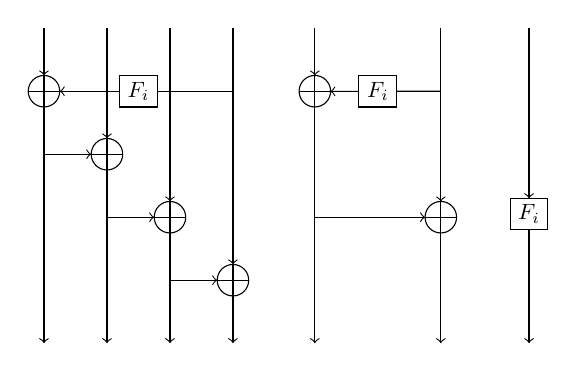
\begin{tikzpicture}[scale=0.8]

\tikzstyle{every node}=[transform shape];

\begin{scope}[xshift=-4cm, shift={(-0.5,-1)}]
\draw[->] (0.5,0) -- ++(0,-1+0.25);
\draw[] (0.5,-1) circle (0.25);
\draw[] (0.25,-1) -- ++(0.5,0);  
\draw[->] (3.5,-1) -- ++(-3+0.25,0);
\draw[fill=white] (1.5+0.2,-1-0.25) rectangle node {\textsf{$F_{i}$}} ++(1-0.4,0.5);
\draw[->] (0.5,-1+0.25) --  ++(0,-4.5+0.25);

\draw[->] (1.5,0) -- ++(0,-2+0.25);
\draw[->] (1.5,-2+0.25) -- ++(0,-3.25);
\draw[->] (0.5,-2) -- ++(1-0.25,0);
\draw[]   (1.5,-2) circle (0.25);
\draw[]   (1.25,-2) -- ++(0.5,0);  

\draw[->] (2.5,0) -- ++(0,-3+0.25);
\draw[->] (2.5,-3+0.25) -- ++(0,-2.25);
\draw[->] (1.5,-3) -- ++(1-0.25,0);
\draw[]   (2.5,-3) circle (0.25);
\draw[]   (2.25,-3) -- ++(0.5,0);  

\draw[->] (3.5,0) -- ++(0,-4+0.25);
\draw[->] (3.5,-4+0.25) -- ++(0,-1.25);
\draw[->] (2.5,-4) -- ++(1-0.25,0);
\draw[]   (3.5,-4) circle (0.25);
\draw[]   (3.25,-4) -- ++(0.5,0);  
\end{scope}

\begin{scope}[xshift=1cm, shift={(-1.2,-1)}]
\draw[->] (0.5,0) -- ++(0,-1+0.25);
\draw[] (0.5,-1) circle (0.25);
\draw[] (0.25,-1) -- ++(0.5,0);  
\draw[->] (2.5,-1) --++(-1.7544,-0.0019);
\draw[fill=white] (1.2,-1-0.25) rectangle node {\textsf{$F_{i}$}} ++(1-0.4,0.5);
\draw[->] (0.5,-1+0.25) --  ++(0,-4.5+0.25);

\draw[->] (0.5,-3)--(2.25,-3);
\draw[->] (2.5,0) -- ++(0,-3+0.25);
\draw[->] (2.5,-3+0.25) -- ++(0,-2.25);
\draw[]   (2.5,-3) circle (0.25);
\draw[]   (2.25,-3) -- ++(0.5,0);  
\end{scope}

\draw [->](3.7,-1) -- (3.7,-3.7);
\draw[fill=white] (3.4,-4.2) rectangle node {\textsf{$F_{i}$}} (4,-3.7);
\draw [->](3.7,-4.2) -- (3.7,-6);
\end{tikzpicture}        
\caption{یک دور از الگوریتم توسیع  کلید  
\en{SR}}
\label{fig:SR_keyschedule}
\end{center}
\end{figure}
کلید اصلی 
$\text{\en{SR}}(n,r,c,e)$
یک کلید 
$rce$
بیتی است که به‌صورت یک آرایه 
$r\times c$
از کلمه‌های 
$e$
بیتی در نظر گرفته می‌شود. کلید هر دور بر اساس کلید دور قبل و به‌صورت نشان داده شده در شکل 
\ref{fig:SR_keyschedule}
به‌دست می‌آید. تابع 
$F_{i}$
در شکل 
\ref{fig:SR_keyschedule}
 یک تابع غیر خطی و در واقع نسخه کوچک‌مقیاس از تابع 
 $F_{i}$
 در الگوریتم توسیع کلید 
\en{AES}
است. این تابع شامل یک انتقال چرخشی کلمات به سمت چپ، اعمال جعبه جانشینی و افزودن یک مقدار ثابت است که در الگوریتم توسیع کلید 
\en{AES}
شرح داده شد، تنها تفاوت آن با الگوریتم توسیع کلید 
\en{AES}
در ثابت‌ها و نگاشت‌های تشکیل‌دهنده جعبه جانشینی است که به‌طور خلاصه در جدول 
\ref{tab:SR_KeySchedule_Const_Summary}
آمده است. 
\begin{table}
\begin{center}
\begin{tabular}{||c||c|c|c||}
	\hline
	\rule[-1ex]{0pt}{2.5ex} & &  $\gf(2^{4})$ & $\gf(2^{8})$ \\ 
	\hline 
	\hline
	\rule[-1ex]{0pt}{2.5ex} ثابت دور
	$i$ام 
	که 
	$1\leq i\leq n$.
	  & $\kappa_{i}$ & $\rho^{i-1}$ & $\theta^{i-1}$ \\ 
	\hline 
	\rule[-1ex]{0pt}{2.5ex} ثابت جعبه جانشینی & $d$ & \texttt{0x6} & \texttt{0x63} \\ 
	\hline 
	\rule[-1ex]{0pt}{2.5ex}   معکوس‌گیری در جعبه جانشینی & $z\mapsto z^{-1}$ & 
	معکوس‌گیری در 
	$\gf(2^{4})$
	 &
	 معکوسگیری در 
	 $\gf(2^{8})$ \\ 
	\hline 
	\rule[-1ex]{0pt}{2.5ex} نگاشت خطی در جعبه جانشینی & $z\mapsto L(z)$ &
	 نگاشت خطی 
	 $\gf(2^{4})$
	& نگاشت خطی 
	$\gf(2^{8})$\\ 
	\hline 
\end{tabular} 
\caption{ثابت‌ها و توابع مورد استفاده در الگوریتم توسیع کلید
	$\text{\en{SR}}(n,r,c,e)$}
\label{tab:SR_KeySchedule_Const_Summary}
\end{center}
\end{table}
جزئیات بیشتر راجع به  الگوریتم توسیع کلید  در بخش استخراج معادلات الگوریتم توسیع کلید آمده است. اکنون آماده‌ایم تا به استخراج معادلات 
\en{AES}
و 
\en{SR}
بپردازیم. در استخراج معادلات دو رویکرد وجود دارد. در رویکرد اول معادلات  روی 
$\gf(2)$
و در رویکرد دوم معادلات  روی 
$\gf(2^{e})$
استخراج می‌شوند که ما در ادامه  نحوه استخراج معادلات بر اساس رویکرد اول را شرح می‌دهیم. 
\subsubsection*{استخراج معادلات 	\en{SR}	و \en{AES} روی $\gf(2)$}
می‌دانیم  
\en{SR}
یک خانواده پارامتری است که 
\en{AES-128}
حالت خاصی از آن است،  لذا بدون کاستن از کلیت، بحث را با 
$\text{\en{SR}}(n,r,c,e)$
ادامه می‌دهیم. تا کنون برای توضیح 
\en{AES}
و 
\en{SR}، 
قالب داده و زیرکلیدها را به‌صورت آرایه‌های دو بعدی در نظر گرفتیم، ولی ‌در این بخش برای  استخراج معادلات حاکم بر 
$\text{\en{SR}}(n,r,c,e)$
 قالب داده و زیرکلید‌ها را به‌صورت بردار‌های ستونی
 $rce$
 بیتی در نظر می‌گیریم. 

همان‌طور که در بخش قبل مشاهده شد، الگوریتم رمز قالبی 
\en{SR}
دارای دو بخش است که عبارتند از بخش توسیع کلید و بخش رمزنگاری، که معادلات هر یک از این بخش‌ها را جداگانه استخراج خواهیم کرد.  در استخراج معادلات بخش رمزنگاری فرض می‌کنیم متن اصلی و رمزشده متناظر با آن معلوم هستند و لذا آن‌ها را به عنوان مقادیر ثابت معادلات در نظر می‌گیریم. مجهولات یا متغیرهای معادله‌های به‌دست آمده از مرحله رمزنگاری، عبارتند از بیت‌های کلید به‌علاوه بیت‌های داده در مراحل میانی الگوریتم رمزنگاری. به‌این ترتیب با استفاده از هر زوج متن اصلی-رمزشده یک دستگاه متفاوت برای مرحله رمزنگاری به‌دست می‌آید. دستگاه معادلات استخراج شده برای الگوریتم توسیع کلید فقط بر حسب بیت‌های کلید و متغیرهای جاری وابسته به بیت‌های کلید خواهد بود و لذا این دستگاه معادلات، مستقل از زوج متن‌های اصلی-رمزشده که در اختیار داریم برای تمام رمزنگاری‌ها تحت یک کلید، مشترک خواهد بود. 

در دستگاه معادلات بخش رمزنگاری،  متغیرهای متناظر با بیت‌های ورودی و خروجی مرحله معکوس‌گیری در جعبه جانشینی را به‌ترتیب با 
$w_{ijl}$
و 
$x_{ijl}$
و بیت‌های کلید را با 
$k_{ijl}$
نمایش می‌دهیم که 
$i$
شماره دور، 
$j$
شماره کلمه و 
$l$
شماره بیت در آن کلمه است. در ادامه  برای سهولت گاهی از دو و گاهی فقط از یک اندیس استفاده می‌کنیم. برای مثال 
$x_{ij}$
نشان‌دهنده کلمه 
$j$
 ام از خروجی مرحله معکوس‌گیری  دور 
 $i$
 ام است، به همین ترتیب 
 $x_{i}$
 نشان‌دهنده بردار خروجی مرحله معکوس‌گیری دور 
 $i$ام
است. 

تنها مرحله غیر آفین در تابع دور 
\en{SR}
مرحله معکوس‌گیری در جعبه جانشینی است که ابتدا نحوه استخراج معادلات در این قسمت را شرح می‌دهیم. قالب داده در هر دور 
$\text{\en{SR}}(n,r,c,e)$
به صورت بسته‌های 
$e$
بیتی وارد جعبه جانشینی می‌شود. بنابراین کافی است که نحوه استخراج روابط چندجمله‌ای بین ورودی و خروجی مرحله معکوس‌گیری، به ازای یک ورودی دلخواه 
$e$
بیتی را بدانیم. فرض کنید بردار ورودی و خروجی مرحله معکوس‌گیری را به ترتیب با 
$w = (w_{0},\ldots,w_{e-1})^{T}$
و 
$x = (x_{0},\ldots,x_{e-1})^{T}$
نمایش دهیم. همچنین فرض کنید چندجمله‌ای‌های متناظر با 
$w$
و 
$x$
در 
$\gf(2^{e})$
را با 
$x = \sum_{i = 0}^{e-1}x_{i}t^{i}$
و
$y = \sum_{j = 0}^{e-1}y_{j}t^{j}$
نمایش دهیم که 
$t$
ریشه‌ی چندجمله‌ای تحویل‌ناپذیر مورد نظر در 
$\gf(2)[x]$
 برای تعریف 
$\gf(2^{e})$
است. در این‌صورت به ازای هر 
$w\neq (0,\ldots,0)$
داریم
$$x = I(w)\Rightarrow (\sum_{i = 0}^{e-1}x_{i}t^{i})*(\sum_{j = 0}^{e-1}y_{j}t^{j}) = \sum_{k = 1}^{e-1}0*t^{k} + 1.$$
با توجه به این‌که ضرایب چند‌جمله‌ای طرف راست و چپ رابطه فوق باید با هم برابر باشند، 
$e$
رابطه‌ی چندجمله‌ای بین متغیرهای 
$w_{i}$
و
$x_{j}$
به‌دست می‌آید. برای مثال در 
\en{AES}
که 
$e = 8$
این معادلات را با استفاده از نرم‌افزار سیج به‌دست آورده‌ایم که در زیر مشاهده می‌کنید.
\begin{equation*}
{\footnotesize \begin{split}
	1 =& w_{0} x_{0} + w_{1} x_{7} + w_{2} x_{6} + w_{3} x_{5} + w_{4} x_{4}\\
	&+w_{5} x_{3} + w_{5} x_{7} + w_{6} x_{2} + w_{6} x_{6} + w_{6} x_{7}\\
	&+w_{7} x_{1} + w_{7} x_{5} + w_{7} x_{6}\\
	0 =& w_{0} x_{1} + w_{1} x_{0} + w_{1} x_{7} + w_{2} x_{6} + w_{2} x_{7} \\
	&+w_{3} x_{5} + w_{3} x_{6} + w_{4} x_{4} + w_{4} x_{5} + w_{5} x_{3}\\
	&+w_{5} x_{4} + w_{5} x_{7} + w_{6} x_{2} + w_{6} x_{3} + w_{6} x_{6}\\
	&+w_{7} x_{1} + w_{7} x_{2} + w_{7} x_{5} + w_{7} x_{7}\\
	0 =& w_{0} x_{2} + w_{1} x_{1} + w_{2} x_{0} + w_{2} x_{7} + w_{3} x_{6} \\
	&+w_{3} x_{7} + w_{4} x_{5} + w_{4} x_{6} + w_{5} x_{4} + w_{5} x_{5}\\
	&+w_{6} x_{3} + w_{6} x_{4} + w_{6} x_{7} + w_{7} x_{2} + w_{7} x_{3}\\
	&+w_{7} x_{6}\\
	0 =& w_{0} x_{3} + w_{1} x_{2} + w_{1} x_{7} + w_{2} x_{1} + w_{2} x_{6} \\
	&+w_{3} x_{0} + w_{3} x_{5} + w_{3} x_{7} + w_{4} x_{4} + w_{4} x_{6}\\
	&+w_{4} x_{7} + w_{5} x_{3} + w_{5} x_{5} + w_{5} x_{6} + w_{5} x_{7}\\
	&+w_{6} x_{2} + w_{6} x_{4} + w_{6} x_{5} + w_{6} x_{6} + w_{6} x_{7}\\
	&w_{7} x_{1} + w_{7} x_{3} + w_{7} x_{4} + w_{7} x_{5} + w_{7} x_{6}\\
	&+ w_{7} x_{7}\\
	\end{split}}
\quad\quad
{\footnotesize\begin{split}
	0 =& w_{0} x_{4} + w_{1} x_{3} + w_{1} x_{7} + w_{2} x_{2} + w_{2} x_{6}\\
	&+w_{2} x_{7} + w_{3} x_{1} + w_{3} x_{5} + w_{3} x_{6} + w_{4} x_{0}\\
	&+w_{4} x_{4} + w_{4} x_{5} + w_{4} x_{7} + w_{5} x_{3} + w_{5} x_{4}\\
	&+w_{5} x_{6} + w_{6} x_{2} + w_{6} x_{3} + w_{6} x_{5} + w_{7} x_{1}\\
	&+w_{7} x_{2} + w_{7} x_{4} + w_{7} x_{7}\\
	0 =& w_{0} x_{5} + w_{1} x_{4} + w_{2} x_{3} + w_{2} x_{7} + w_{3} x_{2}\\
	&+ w_{3} x_{6} + w_{3} x_{7} + w_{4} x_{1} + w_{4} x_{5} + w_{4} x_{6}\\
	&+ w_{5} x_{0} + w_{5} x_{4} + w_{5} x_{5} + w_{5} x_{7} + w_{6} x_{3}\\
	&+ w_{6} x_{4} + w_{6} x_{6} + w_{7} x_{2} + w_{7} x_{3} + w_{7} x_{5}\\
	0 =& w_{0} x_{6} + w_{1} x_{5} + w_{2} x_{4} + w_{3} x_{3} + w_{3} x_{7}\\
	&+w_{4} x_{2} + w_{4} x_{6} + w_{4} x_{7} + w_{5} x_{1} + w_{5} x_{5}\\
	&+w_{5} x_{6} + w_{6} x_{0} + w_{6} x_{4} + w_{6} x_{5} + w_{6} x_{7}\\
	&+w_{7} x_{3} + w_{7} x_{4} + w_{7} x_{6}\\
	0 =& w_{0} x_{7} + w_{1} x_{6} + w_{2} x_{5} + w_{3} x_{4} + w_{4} x_{3}\\
	&+w_{4} x_{7} + w_{5} x_{2} + w_{5} x_{6} + w_{5} x_{7} + w_{6} x_{1}\\
	&+w_{6} x_{5} + w_{6} x_{6} + w_{7} x_{0} + w_{7} x_{4} + w_{7} x_{5}\\
	&+w_{7} x_{7}\\
	\end{split}}
\end{equation*}
تمام روابط فوق به جز معادله اول که مقدار ثابت سمت راست آن ۱ است، به ازای همه مقادیر 
$w, x\in\gf(2)^{e}$
برقرار و لذا با احتمال ۱ درست هستند. معادله اول که مقدار ثابت سمت چپ آن ۱ است زمانی برقرار است که 
$w \neq (0,\ldots,0)^{T}$، 
بنابراین این رابطه با احتمال 
$\frac{255}{256}$
درست است. اگر ورودی و خروجی نگاشت معکوس‌گیری را به‌صورت چندجمله‌ا‌های 
$w, x\in \gf(2^{e})$
در نظر بگیریم داریم 
$1 = xw$. 
حال اگر طرفین رابطه 
$1 = xw$
را در 
$w$
(یا 
$x$)
ضرب کنیم، به معادله 
$w = xw^{2}$
(یا 
$x = x^{2}w$)
می‌رسیم که به ازای هر 
$w\in\gf(2^{e})$
برقرار است. بنابراین   با ضرب پی‌درپی طرفین 
$1 = xw$
در 
$x$
(و یا  
$y$)
روابط زیر به‌دست می‌آید.
\begin{align*}
{\small \fa w\in \gf(2^{e}) : \left \{ \begin{array}{l}
w = xw^{2}\\
w^{2} = x^{2}w^{4}\\
\vdots\\
w^{2^{e-1}} = x^{2^{e-1}}w^{2^{e}} = x^{2^{e-1}}w\\
\end{array} \right.}
&
\quad
{\small\fa w\in \gf(2^{e}) : \left \{ \begin{array}{l}
x = x^{2}w\\
x^{2} = x^{4}w^{2}\\
\vdots\\
x^{2^{e-1}} = x^{2^{e}}w^{2^{e-1}} = xw^{2^{e-1}}
\end{array} \right.}
\end{align*} 
با برابر قرار دادن ضرایب چندجمله‌ای‌های طرفین هر یک  رابطه‌های 
${\small w^{2^{e-1}} = x^{2^{e-1}}w}$
و 
${\small x^{2^{e-1}} = xw^{2^{e-1}}}$
 در مجموع 
$2e$
 معادله چندجمله‌ای دیگر به‌دست می‌آید. بنابراین در مجموع 
 $3e$
 معادله  به‌دست می‌آید که یکی از این معادلات که ثابت سمت چپ آن ۱ است  زمانی درست است که 
$w \neq 0$، 
و در نتیجه با احتمال 
$1 - \frac{1}{2^{e}}$
و مابقی با احتمال ۱ درست هستند.  در 
{\small \en{AES}}
که 
{\small $e = 8$}،
 با برابر قرار دادن ضرایب چندجمله‌ای‌های طرفین رابطه 
$w^{128} = x^{128}w$
معادلات زیر به‌دست می‌آید. 
\begingroup
\allowdisplaybreaks
\begin{equation*}
{\footnotesize \begin{split}
	0 =& w_{0} x_{0} + w_{0} x_{3} + w_{0} x_{5} + w_{0} x_{7} + w_{0} + w_{1}\\
	&x_{1} + w_{1} x_{3} + w_{1} x_{5} + w_{1} x_{7} + w_{2} x_{1} + w_{2}\\
	&x_{3} + w_{2} x_{5} + w_{3} x_{1} + w_{3} x_{3} + w_{3} + w_{4} x_{1} +\\
	&w_{4} x_{7} + w_{5} x_{5} + w_{5} x_{6} + w_{5} x_{7} + w_{5} + w_{6}\\
	&x_{3} + w_{6} x_{4} + w_{6} x_{5} + w_{6} x_{7} + w_{7} x_{1} + w_{7}\\
	&x_{2} + w_{7} x_{3} + w_{7} x_{5} + w_{7}\\
	0 =& w_{0} x_{1} + w_{0} x_{2} + w_{0} x_{3} + w_{1} x_{0} + w_{1} x_{1} +\\
	&w_{1} + w_{2} x_{7} + w_{2} + w_{3} x_{5} + w_{3} + w_{4} x_{3} + w_{4}\\
	&x_{7} + w_{5} x_{1} + w_{5} x_{5} + w_{5} x_{6} + w_{6} x_{3} + w_{6}\\
	&x_{4} + w_{6} x_{6} + w_{7} x_{1} + w_{7} x_{2} + w_{7} x_{4} + w_{7}\\
	&x_{7}\\
	0 =& w_{0} x_{3} + w_{0} x_{4} + w_{0} x_{5} + w_{1} x_{1} + w_{1} x_{2} +\\
	&w_{1} x_{3} + w_{2} x_{0} + w_{2} x_{1} + w_{3} x_{7} + w_{3} + w_{4}\\
	&x_{5} + w_{4} + w_{5} x_{3} + w_{5} x_{7} + w_{5} + w_{6} x_{1} + w_{6}\\
	&x_{5} + w_{6} x_{6} + w_{7} x_{3} + w_{7} x_{4} + w_{7} x_{6}\\
	0 =& w_{0} x_{1} + w_{0} x_{3} + w_{0} x_{6} + w_{1} x_{1} + w_{1} x_{4} +\\
	&w_{1} x_{7} + w_{1} + w_{2} x_{2} + w_{2} x_{5} + w_{3} x_{0} + w_{3}\\
	&x_{3} + w_{3} + w_{4} x_{1} + w_{5} x_{6} + w_{5} x_{7} + w_{6} x_{4} +\\
	&w_{6} x_{5} + w_{6} + w_{7} x_{2} + w_{7} x_{3} + w_{7} x_{6}\\
	0 =& w_{0} x_{1} + w_{0} x_{7} + w_{1} x_{5} + w_{1} x_{6} + w_{1} x_{7} +\\
	&w_{1} + w_{2} x_{3} + w_{2} x_{4} + w_{2} x_{5} + w_{2} x_{7} + w_{3}\\
	&x_{1} + w_{3} x_{2} + w_{3} x_{3} + w_{3} x_{5} + w_{4} x_{0} + w_{4}\\
	&x_{1} + w_{4} x_{3} + w_{4} x_{7} + w_{5} x_{1} + w_{5} x_{5} + w_{5}\\
	&x_{6} + w_{5} x_{7} + w_{6} x_{3} + w_{6} x_{4} + w_{6} x_{5} + w_{6}\\
	&x_{6} + w_{7} x_{1} + w_{7} x_{2} + w_{7} x_{3} + w_{7} x_{4} + w_{7}\\
	\end{split}}
\quad\quad
{\footnotesize\begin{split}
	0 =& w_{0} x_{1} + w_{0} x_{3} + w_{1} x_{1} + w_{1} x_{7} + w_{1} + w_{2}\\
	&x_{5} + w_{2} x_{6} + w_{2} x_{7} + w_{3} x_{3} + w_{3} x_{4} + w_{3}\\
	&x_{5} + w_{3} x_{7} + w_{3} + w_{4} x_{1} + w_{4} x_{2} + w_{4} x_{3} +\\
	&w_{4} x_{5} + w_{5} x_{0} + w_{5} x_{1} + w_{5} x_{3} + w_{5} x_{7} +\\
	&w_{6} x_{1} + w_{6} x_{5} + w_{6} x_{6} + w_{6} x_{7} + w_{7} x_{3} +\\
	&w_{7} x_{4} + w_{7} x_{5} + w_{7} x_{6}\\
	0 =& w_{0} x_{1} + w_{0} x_{3} + w_{0} x_{5} + w_{1} x_{1} + w_{1} x_{3} +\\
	&w_{1} + w_{2} x_{1} + w_{2} x_{7} + w_{3} x_{5} + w_{3} x_{6} + w_{3}\\
	&x_{7} + w_{3} + w_{4} x_{3} + w_{4} x_{4} + w_{4} x_{5} + w_{4} x_{7} +\\
	&w_{5} x_{1} + w_{5} x_{2} + w_{5} x_{3} + w_{5} x_{5} + w_{5} + w_{6}\\
	&x_{0} + w_{6} x_{1} + w_{6} x_{3} + w_{6} x_{7} + w_{7} x_{1} + w_{7}\\
	&x_{5} + w_{7} x_{6} + w_{7} x_{7}\\
	0 =& w_{0} x_{1} + w_{0} x_{3} + w_{0} x_{5} + w_{0} x_{7} + w_{1} x_{1} +\\
	&w_{1} x_{3} + w_{1} x_{5} + w_{1} + w_{2} x_{1} + w_{2} x_{3} + w_{3}\\
	&x_{1} + w_{3} x_{7} + w_{3} + w_{4} x_{5} + w_{4} x_{6} + w_{4} x_{7} +\\
	&w_{5} x_{3} + w_{5} x_{4} + w_{5} x_{5} + w_{5} x_{7} + w_{5} + w_{6}\\
	&x_{1} + w_{6} x_{2} + w_{6} x_{3} + w_{6} x_{5} + w_{7} x_{0} + w_{7}\\
	&x_{1} + w_{7} x_{3} + w_{7} x_{7} + w_{7}\\
	\end{split}}
\end{equation*}
\endgroup
همچنین با برابر قرار دادن ضرایب چندجمله‌ای‌های طرفین رابطه 
$x^{128} = xw^{128}$
به معادله‌های زیر دست می‌یابیم. 
\begin{equation*}
{\footnotesize \begin{split}
	0 =& w_{0} x_{0} + w_{1} x_{1} + w_{1} x_{2} + w_{1} x_{3} + w_{1} x_{4} +\\
	& w_{1} x_{7} + w_{2} x_{7} + w_{3} x_{0} + w_{3} x_{1} + w_{3} x_{2} +\\
	&w_{3} x_{3} + w_{3} x_{6} + w_{3} x_{7} + w_{4} x_{6} + w_{5} x_{0} +\\
	&w_{5} x_{1} + w_{5} x_{2} + w_{5} x_{5} + w_{5} x_{6} + w_{5} x_{7} +\\
	&w_{6} x_{5} + w_{7} x_{0} + w_{7} x_{1} + w_{7} x_{4} + w_{7} x_{5} +\\
	&w_{7} x_{6} + x_{0} + x_{3} + x_{5} + x_{7}\\
	0 =& w_{0} x_{1} + w_{1} x_{0} + w_{1} x_{1} + w_{1} x_{5} + w_{1} x_{7} +\\
	&w_{2} x_{0} + w_{2} x_{7} + w_{3} x_{0} + w_{3} x_{4} + w_{3} x_{6} +\\
	&w_{4} x_{6} + w_{4} x_{7} + w_{5} x_{3} + w_{5} x_{5} + w_{6} x_{5} +\\
	&w_{6} x_{6} + w_{7} x_{2} + w_{7} x_{4} + w_{7} x_{7} + x_{1} + x_{2} +\\
	&x_{3}\\
	0 =& w_{0} x_{2} + w_{1} x_{1} + w_{1} x_{2} + w_{1} x_{6} + w_{2} x_{1} +\\
	&w_{3} x_{0} + w_{3} x_{1} + w_{3} x_{5} + w_{3} x_{7} + w_{4} x_{0} +\\
	&w_{4} x_{7} + w_{5} x_{0} + w_{5} x_{4} + w_{5} x_{6} + w_{6} x_{6} +\\
	&w_{6} x_{7} + w_{7} x_{3} + w_{7} x_{5} + x_{3} + x_{4} + x_{5}\\
	0 =& w_{0} x_{3} + w_{1} x_{0} + w_{1} x_{1} + w_{1} x_{4} + w_{2} x_{2} +\\
	&w_{2} x_{7} + w_{3} x_{0} + w_{3} x_{3} + w_{3} x_{7} + w_{4} x_{1} +\\
	&w_{4} x_{6} + w_{5} x_{2} + w_{5} x_{6} + w_{6} x_{0} + w_{6} x_{5} +\\
	&w_{6} x_{7} + w_{7} x_{1} + w_{7} x_{5} + x_{1} + x_{3} + x_{6}\\
	\end{split}}
\quad\quad
{\footnotesize\begin{split}
	0 =& w_{0} x_{4} + w_{1} x_{0} + w_{1} x_{3} + w_{1} x_{4} + w_{1} x_{5} +\\
	&w_{1} x_{7} + w_{2} x_{3} + w_{2} x_{7} + w_{3} x_{2} + w_{3} x_{3} +\\
	&w_{3} x_{4} + w_{3} x_{6} + w_{3} x_{7} + w_{4} x_{2} + w_{4} x_{6} +\\
	&w_{4} x_{7} + w_{5} x_{1} + w_{5} x_{2} + w_{5} x_{3} + w_{5} x_{5} +\\
	&w_{5} x_{6} + w_{6} x_{1} + w_{6} x_{5} + w_{6} x_{6} + w_{7} x_{0} +\\
	&w_{7} x_{1} + w_{7} x_{2} + w_{7} x_{4} + w_{7} x_{5} + x_{1} + x_{7}\\
	0 =& w_{0} x_{5} + w_{1} x_{0} + w_{1} x_{1} + w_{1} x_{4} + w_{1} x_{5} +\\
	&w_{1} x_{6} + w_{2} x_{4} + w_{3} x_{0} + w_{3} x_{3} + w_{3} x_{4} +\\
	&w_{3} x_{5} + w_{3} x_{7} + w_{4} x_{3} + w_{4} x_{7} + w_{5} x_{2} +\\
	&w_{5} x_{3} + w_{5} x_{4} + w_{5} x_{6} + w_{5} x_{7} + w_{6} x_{2} +\\
	&w_{6} x_{6} + w_{6} x_{7} + w_{7} x_{1} + w_{7} x_{2} + w_{7} x_{3} +\\
	&w_{7} x_{5} + w_{7} x_{6} + x_{1} + x_{3}\\
	0 =& w_{0} x_{6} + w_{1} x_{0} + w_{1} x_{1} + w_{1} x_{2} + w_{1} x_{5} +\\
	&w_{1} x_{6} + w_{1} x_{7} + w_{2} x_{5} + w_{3} x_{0} + w_{3} x_{1} +\\
	&w_{3} x_{4} + w_{3} x_{5} + w_{3} x_{6} + w_{4} x_{4} + w_{5} x_{0} +\\
	&w_{5} x_{3} + w_{5} x_{4} + w_{5} x_{5} + w_{5} x_{7} + w_{6} x_{3} +\\
	&w_{6} x_{7} + w_{7} x_{2} + w_{7} x_{3} + w_{7} x_{4} + w_{7} x_{6} +\\
	&w_{7} x_{7} + x_{1} + x_{3} + x_{5}\\
	0 =& w_{0} x_{7} + w_{1} x_{0} + w_{1} x_{1} + w_{1} x_{2} + w_{1} x_{3} +\\
	&w_{1} x_{6} + w_{1} x_{7} + w_{2} x_{6} + w_{3} x_{0} + w_{3} x_{1} +\\
	&w_{3} x_{2} + w_{3} x_{5} + w_{3} x_{6} + w_{3} x_{7} + w_{4} x_{5} +\\
	&w_{5} x_{0} + w_{5} x_{1} + w_{5} x_{4} + w_{5} x_{5} + w_{5} x_{6} +\\
	&w_{6} x_{4} + w_{7} x_{0} + w_{7} x_{3} + w_{7} x_{4} + w_{7} x_{5} +\\
	&w_{7} x_{7} + x_{1} + x_{3} + x_{5} + x_{7}\\
	\end{split}}
\end{equation*}
به این‌ترتیب در مجموع ۲۴ معادله مربعی برای مرحله معکوس‌گیری توسیع‌یافته در 
\en{AES}
به‌دست می‌آید، که ۲۳تای آن‌ها با احتمال ۱ و آن‌معادله‌ای که مقدار ثابت سمت چپ آن ۱ است با احتمال 
$\frac{255}{256}$
درست است.  کورتوا و پیپشیک در 
\cite{courtois2002cryptanalysis}
نشان دادند  که ۲۳ معادله‌ای که با احتمال ۱ درست هستند، مستقل خطی‌هستند یا به عبارت دیگر ماتریس ضرایب آن‌ها تحت یک ترتیب یکجمله‌ای دلخواه معکوس‌پذیر است. 

در ادامه نشان می‌دهیم که همه‌ی مراحل بعد از مرحله معکوس‌گیری در تابع دور 
\en{SR}
را می‌توان با یک نگاشت آفین بیان کرد و به این ترتیب کار استخراج معادلات به سهولت صورت می‌گیرد. مرحله بعد از معکوس‌گیری عبارت‌است از نگاشت خطی جعبه جانشینی. در بخش‌های قبل ماتریس متناظر با این نگاشت خطی  که در کلمه‌های 
$e$
بیتی ضرب می‌شد را  در جدول 
\ref{tab:summary_of_sr_sbox}
با 
$L_{e}$
نمایش دادیم، به دلیل این که قالب داده را در این قسمت به‌صورت یک بردار ستونی 
$rce$
بیتی در نظر گرفته‌ایم می‌توانیم ماتریس متناظر با نگاشت خطی جعبه جانشینی را با یک ماتریس  بلوکی قطری به‌صورت زیر نمایش دهیم.
$$ 
L = \begin{pmatrix}
[L_{e}]_{e\times e}&[0]_{e\times e}&\cdots&[0]_{e\times e}\\
[0]_{e\times e}&[L_{e}]_{e\times e}&\cdots&[0]_{e\times e}\\
\vdots&\vdots&\vdots&\vdots\\
[0]_{e\times e}&[0]_{e\times e}&\cdots& [L_{e}]_{e\times e}\\
\end{pmatrix}_{rce\times rce}
$$
آخرین مرحله در جعبه جانشینی افزودن مقدار ثابت 
$d\in\gf(2)^{8}$
است که با توجه به قالب در نظر گرفته شده در این قسمت، آن‌را با بردار ستونی 
$\bf{d}$
که حاصل 
$rc$
بار تکرار معدل باینری ثابت 
$d$
در یک ستون است تعویض می‌کنیم. 

مرحله بعد از جعبه جانشینی، انتقال چرخشی است.  می‌دانیم که برداهای سطری آرایه دوبعدی داده در 
$\text{\en{SR}}(n,r,c,e)$
که در معرفی
\en{SR}
شرح داده شد، اعضای فضای بردای 
$c$
بعدی روی 
$\gf(2^{e})$
هستند، به این ترتیب انتقال چرخشی یک‌ واحدی کلمه‌های 
$e$
بیتی یک سطر از آرایه دو بعدی قالب داده به سمت چپ، معادل است با ضرب شدن آن سطر در  ماتریس 
$R\in\mat_{2}(\gf(2^{e}))$
که نسبت به پایه استاندارد به‌صورت زیر تعریف می‌شود. 
$$
\hat{R} = \begin{pmatrix}
0&1_{\gf(2^{e})}&0&0\\
0&0&1_{\gf(2^{e})}&0\\
0&0&0&1_{\gf(2^{e})}\\
1_{\gf(2^{e})}&0&0&0\\
\end{pmatrix}
$$
حال فرض کنید قالب داده در 
$\text{\en{SR}}(n,r,c,e)$
را به‌صورت بردارهای 
$rc$
تایی از اعضای 
$\gf(2^{e})$
در نظر بگیریم و نسبت به پایه استاندارد  به‌صورت زیر نمایش دهیم. 
$$\hat{S} = (S_{0},S_{1},\ldots,S_{rc-1})^{T}\in\gf(2^{e})^{rc}$$
اگر پایه فضای برداری حاوی بردارهای داده در 
\en{SR}
را طوری تغییر دهیم که بردار فوق نسبت به آن‌ پایه به‌صورت زیر نمایش داده شود
$$S = (S_{0},S_{r},\ldots,S_{(c-1)*r},S_{1},S_{r+1},\ldots,S_{(c-1)*r +1},\ldots,S_{r-1},S_{2*(r-1) + 1},\ldots,S_{rc -1})$$
آن‌گاه انتقال چرخشی معادل است با ضرب ماتریس قطری بلوکی زیر در بردار 
$S$. 
$$
\begin{pmatrix}
	I_{c}&[0]_{c}&\cdots&[0]_{c}\\
	[0]_{c}&\hat{R}&\cdots&[0]_{c}\\
	\vdots&\vdots&\vdots&\vdots\\
	[0]_{c}&[0]_{c}&\cdots& \hat{R}^{r-1}\\
\end{pmatrix}_{rc\times rc}\in\mat_{rc}(\gf(2^{e}))
$$
با یک جایگشت مناسب روی سطرها و ستون‌های ماتریس فوق می‌توان ماتریسی یافت که عملیات 
\texttt{ShfitRows}
را نسبت به پایه و ترتیب استاندارد نمایش می‌دهد، این ماتریس را با 
$\bar{R}$
نمایش می‌دهیم. درایه‌های ماتریس 
$\bar{R}$
صفر و یک‌های میدان 
$\gf(2^{e})$
هستند که اگر  صفرها را با ماتریس 
$[0]_{e\times e}\in\mat_{e}(\ffld_{2})$
و یک‌ها را با 
$I_{e}\in\mat_{e}(\ffld_{2})$
جایگزین کنیم به یک ماتریس از 
$\mat_{rce\times rce}(\ffld_{2})$
می‌رسیم که با ضرب آن در بردار داده 
$rce$
بیتی عملیات انتقال چرخشی انجام می‌شود. این ماتریس را که در استخراج معادلات روی 
$\gf(2)$
از آن استفاده می‌کنیم را با 
$\bf{R}$
نمایش می‌دهیم. 

در مرحله 
\texttt{MixColumns}
هر ستون از آرایه داده در ماتریسی که در جدول 
\ref{tab:sr.MixColumns_Matrix}
آمده ضرب می‌شود، درایه‌های این ماترس اعضای میدان 
$\gf(2^{e})$
هستند.  اگر به 
$\gf(2^{e})$
به عنوان یک فضای برداری با بعد 
$e$
 روی 
$\gf(2)$
بنگریم در این‌صورت،  عمل ضرب کردن در یک مقدار ثابت در میدان 
$\gf(2^{e})$
یک نگاشت 
$\gf(2)$
-خطی است که و در نتیجه می‌توان آن‌را با یک ماتریس مربعی از 
$\mat_{e}(\gf(2))$
نمایش داد. برای مثال فرض کنید 
$\theta$
 ریشه چندجمله‌ای تحویل‌ناپذیر 
 $x^{8} + x^{4} + x^{3} + x + 1\in\gf(2)[x]$
 (چندجمله‌ای راین‌دال) باشد، در این صورت 
 $\gf(2)$
 -ماتریس متناظر با عمل ضرب در مقدار ثابت 
 $\theta\in\gf(2)(\theta)$
 نسبت به پایه  
 $\{\theta^{7},\ldots,\theta^{2},\theta, 1\}$
 موسوم به پایه چندجمله‌ای، عبارت است از 
 $$T_{\theta} =  \begin{pmatrix}
 0 & 1 & 0 & 0 & 0 & 0 & 0 & 0 \\
 0 & 0 & 1 & 0 & 0 & 0 & 0 & 0 \\
 0 & 0 & 0 & 1 & 0 & 0 & 0 & 0 \\
 1 & 0 & 0 & 0 & 1 & 0 & 0 & 0 \\
 1 & 0 & 0 & 0 & 0 & 1 & 0 & 0 \\
 0 & 0 & 0 & 0 & 0 & 0 & 1 & 0 \\
 1 & 0 & 0 & 0 & 0 & 0 & 0 & 1 \\
 1 & 0 & 0 & 0 & 0 & 0 & 0 & 0
 \end{pmatrix}$$
بنابراین اگر به‌جای هر یک از مقادیر ثابت ماتریس 
\texttt{MixColumns}
در جدول 
\ref{tab:sr.MixColumns_Matrix}، 
$\gf(2)$
-ماتریس متناظر با آن‌را جایگزین کنیم به یک ماتریس از 
$\mat_{rce}(\ffld_{2})$
می‌رسیم که ضرب آن در بردار داده معادل با عمل 
\texttt{MixColumns}
است، این ماتریس را با 
$\bf{C}$
نمایش می‌دهیم. 

 بنابراین از بین مجموعه عملیات‌هایی که در یک دور از بخش رمزنگاری
 \en{SR}
 یا 
 \en{AES}
 روی داده صورت می‌گیرد تنها مرحله معکوس‌گیری توسیع‌یافته در 
 \texttt{SubByte}
 است که یک عملیات غیر آفین است و  همان‌طور که در شکل  
 \ref{fig:AES_Round_Summary}
 نیز ملاحظه می‌شود مابقی عملیات‌ها را می‌توان در یک نگاشت آفین به‌صورت زیر خلاصه کرد.
 \begin{figure}
 	\centering
 	\includegraphics[width=0.5\linewidth]{AES_Round_Summary}
 	\caption{تقسیم تابع دور 
 		\en{AES}
 		به دو قسمت آفین و غیرآفین}
 	\label{fig:AES_Round_Summary}
 \end{figure}
فرض کنید 
بردار ورودی و خروجی مرحله معکوس‌گیری  در دور 
$i$
را به‌ترتیب با 
$w_{i}$
و 
$x_{i}$
و کلید این دور را با 
$k_{i}$
نمایش دهیم در این صورت تابع دور بخش رمزنگاری در 
$\text{\en{SR}}(n,r,c,e)$
عبارت است از 
$$x_{i-1}\mapsto w_{i} = {\bf CR}({\bf L}(x_{i-1}) + {\bf d}) + k_{i}$$
که نحوه به‌دست آوردن ماتریس‌های 
$\bf{C}, \bf{R}$
و 
$\bf{L}$
را که در فضای 
$\mat_{rce}(\ffld_{2})$
هستند، در بندهای قبل توضیح دادیم. به‌راحتی می‌توان دید که 
$\bf{C* d =  R* d = d}$
که 
$\bf{d}$
همان بردار ثابت 
\en{S-Box}
است. در نتیجه اگر فرض کنیم 
$\bf{M} = \bf{CRL}$
می‌توانیم تابع دور را به‌صورت زیر بیان کنیم
$$x_{i-1}\mapsto w_{i} = {\bf M}  x_{i-1} + k_{i}.$$
معکوس‌گیری کلمه‌به‌کلمه از بردار 
$w_{i}$
را با 
$w_{i}^{(-1)}$
نمایش می‌دهیم که به‌صورت زیر تعریف می‌شود. 
$$x_{i} = w_{i}^{(-1)} = (w_{i,0}^{-1},\ldots,w_{i,rc-1}^{-1})\in\ffld_{2^{8}}^{rc}.$$
به این ترتیب اگر بردار متن اصلی و رمزشده را به‌ترتیب با 
$p$
و 
$c$
نمایش دهیم،  دستگاه معادلات به‌دست آمده برای بخش رمزنگاری
$\text{\en{SR}}(n,r,c,e)$، 
عبارت‌است از 
\begin{equation}
\begin{split}
w_{0} =&  \ p + k_{0}\\
x_{i} =& \ w_{i}^{(-1)}; \ i = 0,\ldots,n-1\\
w_{i} =&  \ {\bf M} x_{i-1} + k_{i} + {\bf d}; \  i = 1,...,n-1\\
c =&  \ {\bf M}x_{n-1} + k_{n} + {\bf d}.
\end{split}
\label{eq:enc_round_of_SR}
\end{equation}
تنها تفاوت 
$\text{\en{SR}}^{\star}(n,r,c,e)$
این است که در دور آخر عملیات 
\texttt{MixColumns}
انجام نمی‌شود ولذا به‌جای ماتریس 
${\bf M}$
در دور آخر از ماتریس 
${\bf M^{\star} = RL}$
استفاده می‌کنیم. 

در الگوریتم توسیع کلید از جعبه جانشینی، انتقال چرخشی و ترکیب کردن با استفاده از عمل جمع استفاده می‌شود که ما نحوه استخراج معادلات در هر یک از این فرآیندها را در بخش رمزنگاری تجربه کردیم. فرض کنید بیت‌های ورودی و خروجی مرحله معکوس‌گیری جعبه جانشینی در دور 
$i$ام 
 الگوریتم توسیع کلید را به‌ترتیب با 
$k_{ijl}$
و 
$s_{ijl}$
نمایش دهیم، که 
$j$
شماره کلمه و 
$l$
شماره بیت را نشان می‌دهد. می‌دانیم که در هر دور از الگوریتم توسیع کلید، فقط  کلمه‌های  ستون آخر  آرایه کلید از جعبه جانشینی عبور می‌کنند. به همین دلیل، تعداد متغیرهای 
$s_{ijl}$
از تعداد متغیرهای
$k_{ijl}$
کمتر است. برای توضیح و همچنین استخراج معادلات الگوریتم توسیع کلید،  همان‌طور که در زیر مشاهده می‌شود، هر زیرکلید یا کلید دور را به صورت یک 
$\gf(2^{e})$
-بردار به‌طول 
$rc$
در نظر می‌گیریم. 
\begin{align*}
\text{کلید اولیه یا اصلی}
&: \ (k_{0,0},\ldots,k_{0,r-1},\ldots,k_{0,r(c-1)},\ldots,k_{0,rc-1})^{T}\\
\text{کلید دور اول}
&: \ (k_{1,0},\ldots,k_{1,r-1},\ldots,k_{1,r(c-1)},\ldots,k_{1,rc-1})^{T}
\\
&\vdots
\\
\text{کلید دور 
	$n$ام}
&: \ (k_{n,0},\ldots,k_{n,r-1},\ldots,k_{n,r(c-1)},\ldots,k_{n,rc-1})^{T}
\end{align*}
همان‌طور که مشاهده می‌شود کلید هر دور به پارامترهای 
$r$
و
$c$
وابسته است و بر اساس کلید دور قبل به‌دست می‌آید که در ادامه چگونگی این کار را به همراه استخراج معادلات الگوریتم توسیع کلیدشرح می‌دهیم. در ضمن هر یک از درایه‌های بردار 
$k_{i,j}$
یک کلمه 
$e$
بیتی است، بنابراین می‌توانیم هر یک از بردارهای فوق را به‌صورت یک 
$\gf(2)$
-بردار به طول 
$rce$
نیز در نظر بگیریم. 
\paragraph*{توسیع کلید  وقتی 
	$r = 1$}
$$s_{i-1,0} = k_{i-1,c-1}^{-1}.$$
\begin{itemize}
	\item[-]
	یک ستون 
	($r = 1, c = 1$).
	$$(k_{i,0}) = (L(s_{i-1,0})) + (d) + (\kappa_{i}).$$
	\item[-]
	بیش‌از یک ستون
	$(r = 1, c >‌ 1)$.
	$$(k_{i,q}) = (L(s_{i-1,0})) + (d) +‌(\kappa_{i}) + \sum_{t =0}^{q}(k_{i-1,t}).$$
	که 
	$q\in \{0,...,c-1\}$.
\end{itemize}
\paragraph*{توسیع کلید وقتی 
	$r = 2$}
$$s_{i-1,0} = k_{i-1,2c-1}^{-1}, \ s_{i-1,1} = k_{i-1,2c-2}^{-1}.$$
\begin{itemize}
	\item[-]
	یک‌ستون 
	$(r = 2, c = 1)$.
	$$
	\begin{pmatrix}
	k_{i,0}\\
	k_{i,1}\\
	\end{pmatrix} = 
	\begin{pmatrix}
	L(s_{i-1,0})\\
	L(s_{i-1,1})\\
	\end{pmatrix} + 
	\begin{pmatrix}
	d\\
	d\\
	\end{pmatrix} +
	\begin{pmatrix}
	\kappa_{i}\\
	0\\
	\end{pmatrix}.
	$$
	\item[-]
	بیش از یک ستون 
	$(r = 2, c > 1)$.
	$$
	\begin{pmatrix}
	k_{i,rq}\\
	k_{i,rq+1}\\
	\end{pmatrix} = 
	\begin{pmatrix}
	L(s_{i-1,0})\\
	L(s_{i-1,1})\\
	\end{pmatrix} + 
	\begin{pmatrix}
	d\\
	d\\
	\end{pmatrix} + 
	\begin{pmatrix}
	\kappa_{i}\\
	0\\
	\end{pmatrix} + 
	\sum_{t = 0}^{q}
	\begin{pmatrix}
	k_{i-1,rt}\\
	k_{i-1,rt+1}\\
	\end{pmatrix}
	$$
	که 
	$q\in \{0,...,c-1\}$.
\end{itemize}
\paragraph*{توسیع کلید وقتی 
	$r = 4$}
$$s_{i-1,0} = k_{i-1,4c-1}^{-1}, \ s_{i-1,1} = k_{i-1,4c-2}^{-1}, \ s_{i-1,2} = k_{i-1,4c-3}^{-1}, s_{i-1,3} = k_{i-1,4c-4}^{-1}.$$
\begin{itemize}
	\item[-]
	یک ستون 
	$(r = 4, c = 1)$.
	$$
	\begin{pmatrix}
	k_{i,0}\\
	k_{i,1}\\
	k_{i,2}\\
	k_{i,3}\\
	\end{pmatrix} = 
	\begin{pmatrix}
	L(s_{i-1,0})\\
	L(s_{i-1,1})\\
	L(s_{i-1,2})\\
	L(s_{i-1,3})\\
	\end{pmatrix} + 
	\begin{pmatrix}
	d\\
	d\\
	d\\
	d\\
	\end{pmatrix} + 
	\begin{pmatrix}
	\kappa_{i}\\
	0\\
	0\\
	0\\
	\end{pmatrix}.
	$$
	\item[-]
	بیش از یک ستون 
	$(r = 4, c > 1)$.
	$$
	\begin{pmatrix}
	k_{i,rq}\\
	k_{i,rq+1}\\
	k_{i,rq+2}\\
	k_{i,rqq+3}\\
	\end{pmatrix} = 
	\begin{pmatrix}
	L(s_{i-1,0})\\
	L(s_{i-1,1})\\
	L(s_{i-1,2})\\
	L(s_{i-1,3})\\
	\end{pmatrix} + 
	\begin{pmatrix}
	d\\
	d\\
	d\\
	d\\
	\end{pmatrix} + 
	\begin{pmatrix}
	\kappa_{i}\\
	0\\
	0\\
	0\\
	\end{pmatrix} + 
	\sum_{t = 0}^{q}
	\begin{pmatrix}
	k_{i-1,rt}\\
	k_{i-1,rt+1}\\
	k_{i-1,rt+2}\\
	k_{i-1,rt+3}\\
	\end{pmatrix}
	$$
	که 
	$q\in \{0,...,c-1\}$.
\end{itemize}
در بندهای قبل ضمن توضیح  جزئیات الگوریتم توسیع کلید معادله‌های آفین حاکم بر این الگوریتم را نمایش دادیم. تنها معادلات غیر آفین الگوریتم توسیع کلید، از مرحله معکوس‌گیری جعبه جانشینی منشأ می‌گیرند که روش به‌دست آوردن آن‌ها را در بخش استخراج معادله‌های الگوریتم رمزنگاری شرح دادیم. 

اکنون به شمارش تعداد معادلات به‌دست آمده برای 
$\text{\en{SR}}(n,r,c,e)$
 و تعداد مجهولات دستگاه شامل این معادله‌ها می‌پردازیم. در بخش‌های قبل دیدیم که به ازای هر معکوس‌گیری 
 $3e$
 معادله به‌دست می‌آید که 
 $3e-1$
 تای آن‌ها با احتمال ۱ و یکی از آن‌ها زمانی درست است که معکوس‌گیری از صفر رخ نداده باشد و لذا با احتمال 
 $1-\frac{1}{2^{e}}$
 درست است. اگر رخداد ظاهر نشدن صفر در ورودی جعبه جانشینی در دورهای مختلف توسیع کلید و رمزنگاری را رخدادهایی مستقل فرض کنیم در این‌صورت احتمال عدم رخداد معکوس‌گیری از صفر در الگوریتم رمزنگاری برابر 
 $(1-\frac{1}{2^{e}})^{nrc}$
 و در الگوریتم توسیع کلید برابر 
 $(1-\frac{1}{2^{e}})^{nc}$
 است. ما در شمارش تعداد معادلات، همه 
 $3e$
معادله به‌دست آمده از مرحله معکوس‌گیری را در نظر می‌گیریم. 

طبق دستگاه 
\ref{eq:enc_round_of_SR}، 
از هر دور  الگوریتم رمزنگاری 
$\text{\en{SR}}(n,r,c,e)$، 
$rce$
معادله خطی به‌دست می‌آید. از طرفی چون هر دور الگوریتم رمزنگاری شامل 
$rc$
عملیات معکوس‌گیری است، 
$rc*3e$
معادله مربعی نیز خواهیم داشت.  الگوریتم رمزنگاری شامل
$n$
دور است و لذا 
$n*(rce + 3rce) = 4n*rce$
معادله خواهیم داشت. الگوریتم رمزنگاری شامل یک مرحله آغازین نیز است  که فقط شامل افزودن کلید اصلی به متن اصلی است، بواسطه این  عملیات 
$rce$
معادله دیگر روی 
$\ffld_{2}$
خواهیم داشت. در نتیجه در مجموع 
$(4n+1)*rce$
 معادله از الگوریتم رمزنگاری به‌دست می‌آید. 
 
هر دور از الگوریتم توسیع کلید شامل 
$r$
عملیات معکوس‌گیری است که 
$3re$
معادله مربعی برحسب بیت‌های کلید و متغیرهای 
$s_{ijl}$
تولید می‌کند. از طرفی به ازای هر دور از الگوریتم توسیع کلید 
$rce$
معادله خطی خواهیم داشت. چون الگوریتم توسیع کلید شامل 
$n$ 
دور است، در نتیجه در مجموع 
$n*(rce+3re)$
معادله از الگوریتم توسیع کلید به‌دست می‌آید. 

 اگر متغیرهای متناظر با بیت‌های داده یعنی 
$w_{ijl}$
و 
$x_{ijl}$
را 
\textbf{\textit{متغیرهای حالت}}
و متغیرهای متناظر با بیت‌های کلید یعنی 
$k_{ijl}$ 
را 
\textbf{\textit{متغیرهای کلید}}
بنامیم، به ازای هر دور از الگوریتم رمزنگاری 
$\text{\en{SR}}(n,r,c,e)$، 
به تعداد 
$2 r c e$
متغیر حالت برای نمایش ورودی و خروجی مرحله معکوس‌گیری در جعبه جانشینی، و 
$r c e$
متغیر کلید برای نمایش بیت‌های کلید آن دور نیاز  است. بنابراین دستگاهی که برای بخش رمزنگاری  به‌دست می‌آید دارای 
$2 n r c e + (n+1) r c e$
متغیر خواهد بود. 

در هر دور الگوریتم توسیع کلید، 
$r$
بار عمل معکوس‌گیری صورت می‌گیرد که به ازای هر معکوس‌گیری باید 
$e$
متغیر جدید 
($s_{ijl}$)
که نشان‌دهنده  خروجی این مرحله هستند معرفی کنیم. به این ترتیب در مجموع 
$nre$
متغیر جدید بواسطه الگوریتم توسیع کلید تولید می‌شود. در نتیجه در مجموع در کل این معادلات،  
$2nrce + (n+1)rce + nre$
مجهول خواهیم داشت. 
\begin{table}
\centering
\begin{tabular}{||c||c|c|c||}
	\hline
	& تعداد معادلات & تعداد متغیرهای حالت & تعداد متغیرهای کلید  \\ 
	\hline
	\hline
	الگوریتم رمزنگاری & $(4n+1)rce$ & $2nrce$ & $(n+1)rce$ \\ 
	\hline
	الگوریتم توسیع کلید & $nrce+3nre$ & $-$ & $nre$ \\
	\hline 
	مجموع & $(5n+1)rce+3nre$ & $2nrce$ & $(n+1)rce + nre$
\\
\hline
\end{tabular}
\caption{تعداد معادلات استخراج شده از 
	$\text{\en{SR}}(n,r,c,e)$}
\label{tab:number_of_eqs_in_SR}
\end{table} 
به‌عنوان مثال  برای 
\en{AES-128}
که همان 
$\text{\en{SR}}^{\star}(10,4,4,8)$
است، 
$7488$
معادله  و 
$4288$
مجهول روی 
$\ffld_{2}$
به‌دست می‌آید. ص

نرم‌افزار سیج دارای ماژول‌های آماده‌ای برای کار با 
\en{SR}
به‌خصوص استخراج معادلات این سامانه است، برای مثال با استفاده از دستور زیر می‌توانیم معادلات 
\en{AES-128}
را استخراج کنیم کنیم. 
\begin{latin}
\begin{flushleft}
\begin{lstlisting}
sr = mq.SR(10,4,4,8,gf2 = True,polybori=True,
                    allow_zero_inversions = False,star = True)
plaintext = sr.random_element();  key = sr.random_element()
ciphertext = sr(plaintext,key)
time poly_sys, solution = sr.polynomial_system(P = plaintext, C = ciphertext)
print poly_sys
Time: CPU 0.92 s, Wall: 0.92 s
Polynomial Sequence with 7488 Polynomials in 4288 Variables
\end{lstlisting}
\end{flushleft}
\end{latin}
الگوریتم‌های پیاده‌سازی شده در سیج دقیقا مطابق با روش توضیح‌داده شده در بندهای قبل معادلات 
\en{SR}
را استخراج می‌کند.  برای آشنایی با روش استخراج معادلات 
\en{SR}
و 
\en{AES}
روی 
$\gf(2^{8})$
می‌توانید به 
\cite{murphy2002essential}
و 
\cite{cid2006algebraic}
رجوع کنید. 
\section{جبری‌سازی رمزهای دنباله‌ای}
همان‌طور که در فصل اوّل هم آمد، رمزهای دنباله‌ای از دو الگوریتم قطعی به نام‌های الگوریتم آغازسازی و الگوریتم تولید کلید اجرایی تشکیل شده‌اند. الگوریتم تولید کلید اجرایی در واقع، یک ماشین حالت محدود
%\LTRfootnote{finite state machine}
است که حالت اولیه‌ی آن توسط الگوریتم آغازسازی و وابسته به کلید و یک مقدار اولیه، تعیین می‌شود و به عنوان مدل واقعی یک مولد شبه تصادفی در نظر گرفته می‌شود. الگوریتم آغازسازی تنها در آغاز رمزنگاری، با دریافت کلید و یک مقدار اولیه (معمولاً وابسته به متن اصلی) حالت اولیه‌ی الگوریتم تولید کلید اجرایی را محاسبه می‌کند، بنابراین بخش اصلی رمز دنباله‌ای را الگوریتم تولید کلید اجرایی تشکیل می‌دهد.

یک حمله‌ی مرسوم به رمزهای دنباله‌ای حمله‌ی متن اصلی معلوم است. فرض کنید مهاجم، تعداد کافی از بیت‌های متن اصلی و رمزشده را دراختیار داشته باشد، به این ترتیب با جمع نظیر به نظیر بیت‌های متن اصلی و متن رمزشده، بیت‌های کلید اجرایی به‌دست می‌آیند. بنابراین  می‌توان گفت که مهاجم، تعداد کافی از بیت‌های کلید اجرایی را در اختیار دارد.  بر اساس هدف مهاجم، حمله به رمزهای دنباله‌ای را می‌توان به دو نوع تقسیم کرد. در نوع اوّل، هدف به‌دست آوردن مقادیر ورودی الگوریتم آغازسازی، یعنی کلید اصلی و بردار حالت اولیه است و در نوع دوم هدف فقط به‌دست آوردن بیت‌های حالت اولیه‌ی مولد شبه تصادفی یا به عبارت دیگر خروجی الگوریتم آغازسازی است. بنابراین در حمله‌ی نوع  دوم از الگوریتم آغازسازی صرف نظر شده و در واقع این مولد شبه تصادفی است که مورد حمله واقع می‌شود. ما نیز در مثال‌هایی که در ادامه آمده از الگوریتم آغازسازی صرف نظر می‌کنیم و هدفمان به‌دست آوردن بیت‌های حالت اولیه‌ی الگوریتم تولید کلید اجرایی است.

الگوریتم تولید کلید اجرایی، همان طور که در شکل 
\ref{fig:prg}
نمایش داده شده از دو تابع اصلی و چند ثبات یا خانه‌ی حافظه تشکیل شده است. 
%\begin{figure}
%\centering
%\includegraphics[width=0.4\linewidth]{Images/PRG}
%\caption{مولد شبه تصادفی در رمزهای دنباله‌ای}
%\label{fig:prg}
%\end{figure}
\begin{figure}
\begin{center}
\begin{tikzpicture}
\draw (-2,1) node  {} -- (0,1) -- (-0.5,0) -- (-1.5,0) -- cycle;
\node [] at (-1,0.5) {\huge $f$};
\draw[rounded corners=0.1cm]  (-1.5,3) rectangle  node {\huge $S_{t}$} (-0.5,2);
\draw[rounded corners=0.1cm]  (0.5,3) rectangle node {\huge $F$}  (2.5,2);
\draw  (-1,-1.5) circle (0.3);
\draw [] (-1,-1.8) -- (-1,-1.2);
\draw (-1.3,-1.5) node (v1) {} -- (-0.7,-1.5) node (v2) {};
\draw [-latex', line width = 0.4mm] (-1,0) -- (-1, -1.2);
\node [] at (-1.3,-1) {$z_{t}$};
\draw [-latex', line width = 0.4mm] (-1,2) -- (-1,1);
\draw  [-latex', line width = 0.4mm] (-0.25,0.5) -- (1.5,0.5) -- (1.5,2);
\draw  [-latex', line width = 0.4mm] (0.5,2.5) -- (-0.5,2.5);	
\draw [-latex', line width = 0.4mm] (-3,-1.5) node [left] {$p_{t}$} -- (-1.3,-1.5);
\draw [-latex', line width = 0.4mm] (-0.7,-1.5) -- (1,-1.5) node [right] {$c_{t}$} ;
\end{tikzpicture}  
\caption{مولد شبه تصادفی در رمزهای دنباله‌ای}
\label{fig:prg}
\end{center}
\end{figure}
یکی از توابع که تابع حالت نام‌دارد،با دریافت حالت فعلی حالت بعدی ماشین، و دیگری با دریافت حالت فعلی خروجی را مشخص می‌کند.  فرض کنید الگوریتم تولید کلیداجرایی (یا مولد شبه تصادفی)
$G$
دارای 
$l$
ثبات برای نگهداری 
$l$
بیت در حافظه‌ی خود باشد. اگر بردار حالت در لحظه‌ی 
$t$
را با 
{\small $S_{t} = (s_{t,0},...,s_{t,l-1})$}
و تابع حالت را با 
$F$
نمایش دهیم در این‌صورت تغییر حالت ماشین توسط 
$F$
به‌صورت زیر انجام می‌شود:
\begin{align*}
F:&\mathbb{F}_{2}^{l}\rightarrow \mathbb{F}_{2}^{l}\\
S_{t}&\mapsto S_{t+1} = F(S_{t}) \ ; \ S_{t+1} = (s_{t+1,0},s_{t+1,1},...,s_{t+1,l-1}).
\end{align*}
بیت 
$t$
ام از کلید اجرایی نیز توسط تابع 
$f$
به‌صورت زیر تعین می‌شود:
\begin{align*}
f:\mathbb{F}_{2}^{l}&\rightarrow \{0,1\}\\
S_{t}&\mapsto z_{t} = f(S_{t}).
\end{align*}


تابع حالت 
$F$
و تابع 
$f$
که به آن فیلتر هم می‌گوییم، توابعی چندجمله‌ای بر حسب متغیرهای حالت هستند، بنابراین اگر حالت اولیه را با بردار 
$(s_{0},...,s_{l-1})$
نمایش دهیم، بین بیت‌های کلید اجرایی و بردار حالت اولیه روابط چندجمله‌ای  زیر برقرار است.
$$\left \{ \begin{array}{l}
z_{0} = f(s_{0},s_{1},...,s_{l-1})\\
z_{1} = f(F(s_{0},s_{1},...,s_{l-1}))\\
\vdots \\
z_{l-1} = f(F^{l-1}(s_{0},s_{1},...,s_{l-1}))
\end{array} \right.$$
اکنون اگر طبق فرض، مهاجم تعدادی از بیت‌های خروجی 
$z_{t}$
را در اختیار داشته باشد با جایگذاری آن‌ها در روابط فوق به یک دستگاه معادلات چندجمله‌ای می‌رسد که مجهولات آن بیت‌های حالت اولیه است.  بنابراین  مهاجم با حل دستگاه به‌دست آمده، قادر خواهد بود حالت اولیه  الگوریتم تولید کلید اجرایی را به‌دست آورد. 

\subsection{ثبات انتقال با بازخورد خطی}
ثبات انتقال با بازخورد خطّی  
%	\LTRfootnote{LFSR: Linear Feedback Shift Register}
نمونه‌ای ساده از الگوریتم‌های تولید کلید اجرایی است. در این نوع مولد، تابع حالت یک تابع خطّی است و بیت‌های کلید اجرایی بیت‌های موجود در یک رجیستر ثابت از این مولّد هستند. 

به‌صورت دقیق‌تر یک ثبات با بازخورد خطّی با استفاده از چند جمله‌ای بازخورد 
{\small $C(x) = 1- \sum_{i = 1}^{L}x^{i}$}
از 
$\mathbb{F}_{2}[x]$
تعریف می‌شود که 
$L$
طول ثبّات نامیده می‌شود.  این ثبات رشته‌ی حالت اوّلیه 
$(s_{0},s_{1},...,s_{L-1})$
را با استفاده از رابطه‌ی بازگشتی زیر به یک دنباله با طول نامتناهی تبدیل می‌کند:
$$\forall \  t \geq 0 \ : \ s_{t+L} = \sum_{i = 1}^{L-1}c_{i}s_{t+L-i}$$
و دنباله‌ی خروجی آن	عبارت است از:
$(s_{t})_{t\geq 0}$.
شکل 
\ref{fig:lfsr}
یک ثبّات با بازخورد خطّی به طول 
$L$
را نشان می‌دهد. دنباله‌ی خروجی یک ثبات با بازخورد خطی، به‌صورت یکتایی توسط ضرایب چندجمله‌ای بازخورد و حالت اولیه‌ تعیین می‌شود. 
\begin{figure}[h]
	\centering
	\includegraphics[width=0.65\linewidth]{Images/LFSR}
	\caption{ثبّات با بازخورد خطّی به طول $L$}
	\label{fig:lfsr}
\end{figure}
\begin{lemma}
	برای هر
	\lr{LFSR}
	با طول 
	$L$
	و بردار حالت اوّلیه‌ی
	$(s_{0},s_{1},...,s_{L-1})$
	، به ازای هر 
	$t\geq 0$
	ضرایب 
	$\{a_{i}^{t}\}_{i = 0}^{L-1}$
	وجود دارند به طوری که
	$$s_{t} = \sum_{i = 0}^{L-1}a_{i}^{t}s_{i}$$
	یعنی هر بیت حالت ترکیبی خطّی از بیت‌های حالت اوّلیه است.
	
\end{lemma}

\begin{proof}
	فرض کنید 
	$C(x) = 1-\sum_{i = 0}^{L-1}c_{i}x^{i}$
	چند جمله‌ای بازخورد 
	\lr{LFSR}
	و بردار 
	$(s_{0},...,s_{L-1})$
	بردار حالت اوّلیه باشد در این صورت تابع انتقال حالت یک تابع خطّی است که با ماتریس زیر قابل نمایش است
	$$
	C = \begin{pmatrix}
	0 & 0 & 0 & \dots & 0 & c_{L} \\ 
	1 & 0 & 0 & \dots & 0 & c_{L-1} \\ 
	0 & 1 & 0 & \dots & 0 & c_{L-2} \\ 
	\colon & \colon & \colon & \dots & \colon & \colon \\ 
	0 & 0 & 0 & \dots & 1 & c_{1}
	\end{pmatrix} 
	$$
	$t\geq 0$
	$S_{t} = (s_{t},s_{t+1},...,s_{t+L-1})$
	$$F:\{0,1\}^{L}\rightarrow \{0,1\}^{L}$$
	$$S_{t}\mapsto S_{t+1} = C S_{t}$$
	$s_{t}$
	$$s_{t} = S_{0}C^{t}\begin{pmatrix}
	1 \\ 
	0 \\ 
	0 \\ 
	\colon \\ 
	0
	\end{pmatrix} \Longrightarrow \begin{pmatrix}
	a_{0}^{t} \\ 
	a_{1}^{t} \\ 
	a_{2}^{t} \\ 
	\colon \\ 
	a_{L-1}^{t}
	\end{pmatrix} = C^{t} \begin{pmatrix}
	1 \\ 
	0 \\ 
	0 \\ 
	\colon \\ 
	0
	\end{pmatrix}$$
	
\end{proof}

$L$
$s_{t_{1}},...,s_{t_{L}}$
\lr{LFSR}
$L$
را بدانیم و ماتریس  ضرایب 
$A$
که در زیر نمایش داده شده معکوس پذیر باشد، 
$$A = \begin{pmatrix}
a_{0}^{t_{1}} & a_{0}^{t_{2}} & ... & a_{0}^{t_{L}} \\ 
a_{1}^{t_{1}} & a_{1}^{t_{2}} & ... & a_{1}^{t_{L}} \\ 
\colon & \colon & ... & \colon \\ 
a_{L-1}^{t_{1}} & a_{L-1}^{t_{2}} & ... & a_{L-1}^{t_{L}}
\end{pmatrix} $$

به‌راحتی می‌توانیم بردار حالت اوّلیه را با محاسبه‌ی ساده‌ی زیر به‌دست آوریم.

$$S_{0} = (s_{0},...,s_{L-1}) = (s_{t_{1}},...,s_{t_{L}})\begin{pmatrix}
a_{0}^{t_{1}} & a_{0}^{t_{2}} & ... & a_{0}^{t_{L}} \\ 
a_{1}^{t_{1}} & a_{1}^{t_{2}} & ... & a_{1}^{t_{L}} \\ 
\colon & \colon & ... & \colon \\ 
a_{L-1}^{t_{1}} & a_{L-1}^{t_{2}} & ... & a_{L-1}^{t_{L}}
\end{pmatrix}^{-1}$$
طبق لم ‌ زیر احتمال معکوس پذیر بودن ماتریس ضرایب نیز قابل توجه است.
\begin{lemma}
	احتمال این که یک ماتریس تصادفی روی 
	$\mathcal{M}_{n}(\mathbb{F}_{q})$
	معکوس پذیر باشد برابر است با:
	$$\gamma_{q}(n) = Pr\{M\gets \text{\lr{Mat}}_{n}(\mathbb{F}_{q}) \ ; \ M: \text{معکوس پذیر باشد}\} = \prod_{i = 1}^{n}(1-\frac{1}{q^{i}})$$
	$$\lim_{n \to \infty}\gamma_{q}(n) = 1-\frac{1}{q}+\O(\frac{1}{q^{2}}) $$
	که با قرار دادن 
	$q = 2$
	داریم:
	$$\gamma_{q}(\infty) = \prod_{i = 1}^{\infty}(1-\frac{1}{2^{i}}) \approx 0.2887880951$$
\end{lemma}

درسال‌های ‌آغازین قرن بیست‌ویکم، تعدادی از رمزهای دنباله‌ای مورد حملات جدّی قرار گرفتند که از مهم‌ترین آن‌ها می‌توان به رمز دنباله‌ای 
\lr{A5/1}
وحمله‌ی اعمال شده به آن در 
{\small \cite{biryukov2000real}}،
و 
\lr{A5/2}
و تحلیل صورت گرفته روی آن در 
\cite{barkan2003instant}،
اشاره کرد. چنین حمله‌های مؤفقی، زمانی صورت گرفت که این رمزهای دنباله‌ای برای برقراری امنیت سامانه‌ی جهانی ارتباطات همراه، 
%\LTRfootnote{Global System for Mobile Communication}
که میلیون‌ها شهروند اروپایی از آن استفاده می‌کردند، به‌کار گرفته شده بود. این تهدید‌ها سبب شد تا سازمان رمزنگاری اروپایی 
\lr{ECRYPT}
اقدام به برگزاری مسابقه‌ای برای طراحی رمزهای دنباله‌ای کند. این مسابقه که به پروژه‌ی 
\lr{eStream}
معروف است در سال ۲۰۰۴ آغاز شد و در مجموع ۳۴ سامانه‌ی رمز دنباله‌ای به این مسابقه ارسال شدند. سامانه‌های پیشنهادی طی سه مرحله مورد آزمون قرار گرفتند تا این‌که در سال ۲۰۰۸ که پایان مسابقه بود تنها هفت الگوریتم از مرحله‌ی نهایی عبور کرده و به عنوان الگوریتم‌های برتر شناخته شدند. رمزهای دنباله‌ی پیشنهادی در این مسابقه در دو دسته‌ی نرم‌افزار‌مبنا و سخت‌افزار‌مبنا قرار داشتند. یکی از الگوریتم‌های منتخب در این مسابقه رمزدنباله‌ای 
\lr{Trivium}
است که در ادامه  فرآیند جبری‌سازی آن را بررسی می‌کنیم.


\subsection{جبری‌سازی  \lr{Trivium} و \lr{Bivium}}
\begin{figure}
	\centering
	\includegraphics[width=0.6\linewidth]{Images/Trivium}
	\caption{  رمز دنباله‌ای 
		\lr{Trivium}}
	\label{fig:trivium}
\end{figure}
\subsubsection*{معرفی \lr{Trivium}}
\lr{Trivium}، 
یک رمز دنباله‌ای است که  توسط  کانییِری 
\LTRfootnote{Canniere}
و پرینییِل  
\LTRfootnote{Preneel}، 
\cite{canniere2005trivium}
ارائه شد. این رمز دنباله‌ای از یک ثبات انتقال همزمان بیتی به طول ۲۸۸ بیت، برای تولید کلید اجرایی دودویی با حداکثر طول 
$2^{64}$ 
از روی یک کلید 
$80$
بیتی به همراه  یک بردار حالت اولیه 
$80$
بیتی به‌کار می‌رود. مانند اغلب رمزهای دنباله‌ای این فرآیند شامل دو مرحله اصلی است. در مرحله اول که آغازسازی نام‌ دارد، بیت‌های ثبات انتقال  با استفاده از کلید و بردار حالت اولیه مقدار دهی می‌شوند.  در مرحله دوم بیت‌های ثبات انتقال یا همان بیت‌های حالت داخلی  به طور مرتب و پی‌درپی، بر اساس یک تابع  مشخص  از حالت قبلی  به‌روز می‌شوند. این فرآیند تکراری تا زمانی ادامه می‌یابد که به اندازه کافی بیت کلید اجرایی تولید شود. 

ابتدا مرحله دوم یعنی فرآیند به‌روز رسانی بیت‌های حالت داخلی را شرح می‌دهیم. فرض کنید بیت‌های ثبات انتقال را با 
$(s_{0},...,s_{287})$، 
نمایش دهیم و 
$z_{t}$، 
نشان‌دهنده‌ بیت 
$t$ام
کلید اجرایی باشد، در این‌صورت اگر بخواهیم 
$N$
بیت از کلید اجرایی را 
(که 
$N\leq 2^{64}$)
تولید کنیم،  فرآیند به‌روزرسانی مطابق الگوریتم 
\ref{Trivium alg1}، 
صورت می‌گیرد. نمایش تصویری فرآیند به‌روزرسانی بیت‌های حالت داخلی در شکل 
\ref{fig:trivium}، 
نمایش داده شده است. 
\renewcommand{\algorithmicrequire}{\textbf{Input:}}
\renewcommand{\algorithmicensure}{\textbf{Output:}}
\begin{algorithm}
	\caption{الگوریتم به‌روزرسانی  و تولید کلید اجرایی در رمز دنباله‌ای  
		\lr{Trivium}}
		\label{Trivium alg1}
	\begin{latin}
		\begin{algorithmic}[]		
			\FOR{$t = 0,...,N-1$}	
			\STATE $t_{1}\gets s_{65}+ s_{92}$
			\STATE $t_{2}\gets s_{161} + s_{176}$	
			\STATE $t_{3}\gets s_{242} + s_{287}$
			\STATE $z_{t}\gets t_{1} + t_{2} + t_{3}$
			\STATE $t_{1}\gets t_{1} + s_{90}*s_{91} + s_{170}$
			\STATE $t_{2}\gets t_{2} + s_{174}*s_{175} + s_{263}$
			\STATE $t_{3}\gets t_{3} + s_{285}*s_{286} + s_{68}$
			\STATE $(s_{0},...,s_{92})\gets (t_{3},s_{0},...,s_{91})$
			\STATE $(s_{93}, ...,s_{176})\gets (t_{1}, s_{93},...,s_{175})$
			\STATE $(s_{177}, ...,s_{287})\gets (t_{2}, s_{177},...,s_{286})$
			\ENDFOR
		\end{algorithmic}
	\end{latin}
\end{algorithm}
مرحله آغازسازی نیز مطابق الگوریتم 
\ref{Trivium_Initialization}، 
صورت می‌گیرد. 
\begin{algorithm}
\caption{مرحله آغازسازی در رمز دنباله‌ای 
		\lr{Trivium}}
\label{Trivium_Initialization}	
	\begin{latin}
		\begin{algorithmic}[]

			\STATE $(s_{0},...,s_{92}) \gets (K_{0},...,K_{79},0,...,0)$
			\STATE $(s_{93},...,s_{176}) \gets (IV_{0},...,IV_{79},0,...,0)$
			\STATE $(s_{177},...,s_{287}) \gets (0,...,0,1,1,1)$
			\FOR{$0 = 1,...,1151$}	
			\STATE $t_{1} \gets s_{65} + s_{90}*s_{91} + s_{93} + s_{170}$			
			\STATE $t_{2} \gets s_{161} + s_{174}*s_{175} + s_{176} + s_{263}$
			\STATE $t_{3} \gets s_{242} + s_{285}*s_{286} + s_{287} + s_{68}$
			\STATE $(s_{0},...,s_{92})\gets (t_{3},s_{0},...,s_{91})$
			\STATE $(s_{93}, ...,s_{176})\gets (t_{1}, s_{93},...,s_{175})$
			\STATE $(s_{177}, ...,s_{287})\gets (t_{2}, s_{177},...,s_{286})$
			\ENDFOR
		\end{algorithmic}
	\end{latin}
\end{algorithm}

\subsubsection*{معرفی \lr{Bivium}}
\lr{Bivium}، 
نسخه تقلیل‌یافته‌ای از الگوریتم رمزنگاری 
\lr{Trivium} 
است که توسط  رادوم
\LTRfootnote{Raddum}
\cite{raddum2006cryptanalytic}، 
و در  دو نوع 
\lr{A}
و
\lr{B}
ارائه شد. در این سامانه از یک ثبات انتقال همزمان ۱۷۷ بیتی برای تولید کلید اجرایی از روی کلید ۸۰ بیتی و بردار حالت اولیه ۸۰ بیتی استفاده می‌شود. اگر ۱۷۷ بیت حالت داخلی را با 
$(s_{0},...,s_{176})$، 
و بیت 
$t$ام
کلید اجرایی را با 
$z_{t}$، 
نمایش دهیم آن‌گاه،  فرآیند به‌روزرسانی و تولید بیت‌های کلید اجرایی مطابق الگوریتم 
\ref{Bivium_A_B_UpdateFunction}
است. 
\begin{algorithm}
\caption{الگوریتم به‌روزرسانی و تولید کلید اجرایی در رمز دنباله‌ای 
		\lr{Bivium}}
\label{Bivium_A_B_UpdateFunction}	
	\begin{latin}
		\begin{algorithmic}[]						
			\FOR{$t = 0,...,N - 1$}	
			\STATE $t_{1} \gets s_{65} + s_{92}$
			\STATE $t_{2} \gets s_{161} + s_{176}$
			\STATE $z_{t} \gets t_{2} (\text{Variant A}) / t_{1} + t_{2} (\text{Variant B})$
			\STATE $t_{1} \gets t_{1} + s_{90}*s_{91} + s_{170}$
			\STATE $t_{2} \gets t_{2} + s_{174}*s_{175} + s_{69}$
			\STATE $(s_{0},...,s_{92}) \gets (t_{2}, s_{0},...,s_{91})$
			\STATE $(s_{93},...,s_{176}) \gets (t_{1}, s_{93},...,s_{175})$
			\ENDFOR
		\end{algorithmic}
	\end{latin}
\end{algorithm}

فرآیند آغازسازی در 
\lr{Bivium}، 
شبیه 
\lr{Trivium}
است که در الگوریتم 
\ref{Trivium_Initialization}
بیان شد، با این تفاوت که حلقه‌  به‌روزرسانی به‌جای
$4\times 288 = 1152$
مرتبه به تعداد 
$4\times177 = 708$، 
مرتبه تکرار می‌شود. 

\subsubsection*{استخراج معادلات  \lr{Trivium} و \lr{Bivium}}
چون در هر دو الگوریتم مورد بحث، فرآیند آغازسازی هیچ تفاوتی با فرآیند تولید رشته کلید اجرایی ندارد لذا  در هر دو روش  از فرآیند آغازسازی صرف‌ نظر می‌کنیم و هدف ما به‌دست آوردن مقادیر بیت‌های ثبات انتقال بعد از فرآیند آغازسازی و درست در لحظه شروع  تولید رشته کلید اجرایی است. در ضمن فرض بر این است که به تعداد کافی از بیت‌های کلید اجرایی دسترسی داریم.  برای استخراج معادلات این سامانه‌ها دو روش معرفی می‌کنیم. در روش اول معادلات را فقط بر حسب بیت‌های حالت در لحظه شروع تولید کلید اجرایی‌ به‌دست می‌آوریم و متغیر جدیدی معرفی نمی‌کنیم. در روش دوم در هر دور تعدادی متغیر جدید معرفی می‌کنیم به طوری که درجه معادلات استخراج شده همواره حداکثر برابر با ۲ باشد. 

\begin{enumerate}
	\item  
	فرض کنید مقادیر بیت‌های ثبات انتقال در آغاز تولید کلید اجرایی در 
	\lr{Trivium}
	را با 
	$(s_{0},...,s_{287})$، 
	و در 
	\en{Bivium}
	را با 
	$(s_{0},...,s_{176})$، 
	نمایش دهیم. در روش اول  هیچ متغیر جدیدی معرفی نمی‌کنیم و همه معادلات را بر حسب
	$s_{i}$ها 
	که 
	$i\in \{0,...,287\}$
	(یا 
	$i\in \{0,...,176\}$)
	به‌دست می‌آوریم. در این روش تعداد متغیرها ثابت و برابر با طول ثبات انتقال باقی می‌ماند، ولی درجه معادلات و تعداد یکجمله‌ای‌های معادلات استخراج شده رفته رفته افزایش می‌یابد.  برای مثال الگوریتم 
	\en{Trivium}، 
	را در نظر بگیرید.  در این روش در هر دور 
	$z_{i}$
	را که کلید اجرایی تولید شده در دور 
	$i$ام
	الگوریتم  
	\ref{Trivium alg1} 
	است، بر حسب بیت‌های  ثبات  انتقال در لحظه شروع تولید کلید اجرایی به‌دست می‌آوریم. به این‌ ترتیب در  ۶۶ دور اول معادلات خطی هستند، سپس به ازای دور 
	$i\in \{67,...,148\}$
	معادله‌ها از درجه‌ی ۲ و به ازای 
	$i\in \{149,...,214\}$
	معادله‌ها از درجه ۳  و به ازای  
	$i \in \{215,..., 239\}$
	از درجه ۴  هستند و این روند  افزایشی ادامه می‌یابد. برای مثال تعدادی از معادلات به‌دست آمده با این روش در زیر نمایش داده شده است. 
	\begin{align*}
	z_{1} =& s_{65} + s_{92} + s_{161} + s_{176} + s_{242} + s_{287}\\
	z_{2} =& s_{64} + s_{91} + s_{160} + s_{175} + s_{241} + s_{286}\\
	\ \vdots\\
	z_{66} =& s_{0} + s_{27} + s_{96} + s_{111} + s_{177} + s_{222}\\
	z_{67} =& s_{26} + s_{68} + s_{95} + s_{110} + s_{161} + s_{174} s_{175} + s_{176} + s_{221} + s_{242} + s_{263} + s_{285} s_{286} + s_{287}\\
	\ \vdots\\
	z_{148} =& s_{2} + s_{12} s_{13} + s_{27} s_{28} + s_{29} + s_{53} + s_{65} + s_{78} s_{79} + s_{80} + s_{90} s_{91} + s_{92} + s_{93} s_{94} + s_{95}\\
	&+ s_{107} + s_{125} + s_{138} s_{139} + s_{140} + s_{146} + s_{158} + s_{159} s_{160} + s_{161} + s_{170} + s_{182} + s_{188}\\ 
	&+ s_{204} s_{205} + s_{206} + s_{227} + s_{231} s_{232} + s_{233} + s_{248}\\
	z_{149} =& s_{1} + s_{11} s_{12} + s_{26} s_{27} + s_{28} + s_{52} + s_{64} +
	s_{65} s_{93} + s_{77} s_{78} + s_{79} + s_{89} s_{90} + s_{90} s_{91}
	s_{93}\\
	&+ s_{91} + s_{92} s_{93} + s_{93} s_{170} + s_{94} + s_{106} +
	s_{124} + s_{137} s_{138} + s_{139} + s_{145} + s_{157} + s_{158}
	s_{159}\\
	&+ s_{160} + s_{169} + s_{181} + s_{187} + s_{203} s_{204} + s_{205} + s_{226} + s_{230} s_{231} + s_{232} + s_{247}\\
	\ \vdots
	\end{align*}
	همان‌طور که مشاهده می‌شود درجه و تعداد یکجمله‌ای‌های معادلات استخراج شده  با این روش، در دورهای بالاتر افزایش می‌یابد. پس از پیاده‌سازی این روش استخراج، با استفاده از نرم‌افزار سیج، متوجه شدیم که معادلات استخراج شده به ازای دورهای بالاتر آن‌قدر بزرگ هستند که سبب پر شدن حافظه رم کامپیوتر می‌شوند. اگر بتوانیم متغیرهایی را که  به دفعات  در یکجمله‌ای‌های غیر خطی ظاهر می‌شوند،  شناسایی کنیم و بجای آن‌ها مقادیر عددی حدسی قرار دهیم، می‌توانیم تا حدی از حجم یکجمله‌ای‌ها ظاهر شده در معادلات کم کنیم که این کار سبب ساده‌تر شدن حل دستگاه به‌دست آمده خواهد شد. 
	
	\item 
	در روش دوم به ازای هر کلاک (یا هر انتقال ثبات انتقال)، تعدادی متغیر جدید اضافه می‌کنیم. برای فهم بهتر و سادگی پیاده‌سازی این روش، ثبات انتقال 
	\en{Trivium} 
	را به سه ثبات با طول‌های 
	$93, 84$
	و 
	$111$، 
	مطابق شکل 
	\ref{fig:Trivium3Stages}، 
	تقسیم می‌کنیم.  اگر بیت‌های ثبات انتقال در لحظه 
	$t$
	را با  
	$(a_{t},...,a_{t + 92}, b_{t},...,b_{t + 83}, c_{t},..., c_{t + 110})$
	و بیت 
	$t$ام
	کلید اجرایی را با 
	$z_{t}$
	نمایش دهیم، فرآیند آغازسازی، به‌روزرسانی بیت‌های حالت و تولید کلید اجرایی طبق  الگوریتم 
	\ref{Trivium_3_stages}  
	است.
\begin{algorithm}
\caption{الگوریتم رمزنگاری 
		\en{Trivium}}
\label{Trivium_3_stages}	
	\begin{latin}
		\begin{algorithmic}[]
				
			\REQUIRE  $K = (k_{0},...,k_{79}), IV = (v_{0},...,v_{79}), N$
			\ENSURE $Z = (z_{0},...,z_{N - 1})$
			\STATE $(a_{0},...,a_{92},b_{0},...,b_{83},c_{0},...,c_{110})\gets (\underbrace{0,...,0, k_{79},...,k_{0}}_\text{A},\underbrace{0,0,0,0,v_{79},...,v_{0}}_{B},\underbrace{1,1,1,0,...,0}_{C})$
			\FOR{$t = 0,...,1151$}	
			\STATE $a_{t + 93} \gets a_{t + 24} + c_{t + 45} + c_{t} + c_{t + 1}*c_{t + 2}$
			\STATE $b_{t + 84} \gets b_{t + 6} + a_{t + 27} + a_{t} + a_{t + 1}*a_{t + 2}$
			\STATE $c_{t + 111} \gets c_{t + 24} + b_{t + 15} + b_{t} + b_{t + 1}*b_{t + 2}$
			\ENDFOR
			\FOR{$t = 0,...,N-1$}		
			\STATE $z_{t} \gets a_{t} + a_{t + 27} + b_{t} + b_{t + 15} + c_{t} + c_{t + 45}$
			\STATE $a_{t + 93} \gets a_{t + 24} + c_{t + 45} + c_{t} + c_{t + 1}*c_{t + 2}$
			\STATE $b_{t + 84} \gets b_{t + 6} + a_{t + 27} + a_{t} + a_{t + 1}*a_{t + 2}$
			\STATE $c_{t + 111} \gets c_{t + 24} + b_{t + 15} + b_{t} + b_{t + 1}*b_{t + 2}$		
			\ENDFOR
		\end{algorithmic}
	\end{latin}
\end{algorithm}
	
	%\def\svgwidth{\textwidth}
	%\begin{latin}
	%\import{Images/}{Trivium_3_stages_temp.pdf_tex}
	%\end{latin}
	
	
%beging of Trivium_3_Staegs Tikz
\definecolor{c00ffff}{RGB}{0,255,255}
\definecolor{cffffff}{RGB}{255,255,255}
\definecolor{cff00ff}{RGB}{255,0,255}
\definecolor{cffff00}{RGB}{255,255,0}
\definecolor{c0d9cff}{RGB}{13,156,255}
\definecolor{cff6600}{RGB}{255,102,0}
	
\begin{figure}
\begin{center}
\begin{tikzpicture}[y=0.80pt, x=0.80pt, yscale=-0.5, xscale=0.5, inner sep=0pt, outer sep=0pt]
\large %font of texts, you can choose another font or comment it completely
\begin{scope}% layer1
% shift register 1  
\path[draw=black,miter limit=4.00,line width=1.533pt,rounded corners=0.0000cm, shade, top color = green]
(161.3204,138.2501)  rectangle (729.5445,198.3341)--cycle;

% a27 register
\path[draw=black,miter limit=4.00,line width=1.600pt,rounded
corners=0.0000cm, shading = radial, outer color = c00ffff,inner color = white] (399.1494,138.6056) rectangle (439.5025,198.2921);
\coordinate (a) at (399.1494,138.6056);
\coordinate (b) at (439.5025,198.2921);
\path[fill=black,line join=miter,line cap=butt,line width=0.800pt]
($(a)!0.5!(b)$)  node[] (text4164) {$a_{27}$};



% a0 register
\path[draw=black,miter limit=4.00,line width=1.600pt,rounded
corners=0.0000cm, shading = radial, outer color = c00ffff, inner color = white] (688.9927,138.4488) rectangle (729.3458,198.1353);
\coordinate (a) at (688.9927,138.4488);
\coordinate (b) at (729.3458,198.1353);
\path[fill=black,line join=miter,line cap=butt,line width=0.800pt]
($(a)!0.5!(b)$)  node[] (text4148) {$a_{0}$}; 

% a1 register
\path[draw=black,miter limit=4.00,line width=1.600pt,rounded
corners=0.0000cm, shading = radial, outer color = c00ffff, inner color = white] (648.9927,138.4488) rectangle (689.3458,198.1353);
\coordinate (a) at (648.9927,138.4488);
\coordinate (b) at (689.3458,198.1353);
\path[fill=black,line join=miter,line cap=butt,line width=0.800pt]
($(a)!0.5!(b)$)  node[] (text4152) {$a_{1}$};


% a2 register
\path[draw=black,miter limit=4.00,line width=1.600pt,rounded
corners=0.0000cm, shading = radial, outer color = c00ffff, inner color = white] (608.9927,138.4488) rectangle (649.3458,198.1353);
\coordinate (a) at (608.9927,138.4488);
\coordinate (b) at (649.3458,198.1353);
\path[fill=black,line join=miter,line cap=butt,line width=0.800pt]
($(a)!0.5!(b)$)  node[] (text4156) {$a_{2}$};


\begin{scope}[shift={(299.50254,75.9299)},miter limit=4.00,line width=1.600pt]% g7092
% path2399
\path[shift={(0,60.0)},draw=black,fill=cffffff,miter limit=4.00,line
width=1.600pt] (410.0000,172.3622) circle (0.2822cm);

% path2401
\path[draw=black,line join=miter,line cap=butt,miter limit=4.00,even odd
rule,line width=1.600pt] (410.0000,222.3622) -- (410.0000,242.3622);

% path2403
\path[draw=black,line join=miter,line cap=butt,miter limit=4.00,even odd
rule,line width=1.600pt] (400.0000,232.3622) -- (420.0000,232.3622);

\end{scope}
% shift register 2
\path[draw=black,miter limit=4.00,line width=1.481pt,rounded
corners=0.0000cm] (198.9277,418.0612) rectangle (729.0668,478.2095);

% b6 register
\path[draw=black,miter limit=4.00,line width=1.600pt,rounded
corners=0.0000cm, shading = radial, outer color = c00ffff, inner color = white] (499.5025,418.2921) rectangle (539.8557,477.9786);
\coordinate (a) at (499.5025,418.2921);
\coordinate (b) at (539.8557,477.9786);
\path[fill=black,line join=miter,line cap=butt,line width=0.800pt]
($(a)!0.5!(b)$)  node[] (text4184) {$b_{6}$};

% b0 register
\path[draw=black,miter limit=4.00,line width=1.600pt,rounded
corners=0.0000cm, shading = radial, outer color = cff00ff, inner color = white] (688.4828,418.2921) rectangle (728.8360,477.9786);
\coordinate (a) at (688.4828,418.2921);
\coordinate (b) at (728.8360,477.9786);
\path[fill=black,line join=miter,line cap=butt,line width=0.800pt]
($(a)!0.5!(b)$)  node[] (text4172) {$b_{0}$};   

% b1 register
\path[draw=black,fill=cff00ff,miter limit=4.00,line width=1.600pt,rounded
corners=0.0000cm, shading = radial, outer color = cff00ff, inner color = white] (648.4828,418.2921) rectangle (688.8360,477.9786);
\coordinate (a) at (648.4828,418.2921);
\coordinate (b) at (688.8360,477.9786);
\path[fill=black,line join=miter,line cap=butt,line width=0.800pt]
($(a)!0.5!(b)$)  node[] (text4176) {$b_{1}$};

% b2 register
\path[draw=black,miter limit=4.00,line width=1.600pt,rounded
corners=0.0000cm, shading = radial, outer color = cff00ff, inner color = white] (608.4828,418.2921) rectangle (648.8360,477.9786);
\coordinate (a) at (608.4828,418.2921);
\coordinate (b) at (648.8360,477.9786);
\path[fill=black,line join=miter,line cap=butt,line width=0.800pt]
($(a)!0.5!(b)$)  node[] (text4180) {$b_{2}$};

% path3205
\path[draw=black,line join=miter,line cap=butt,miter limit=4.00,even odd
rule,line width=1.600pt, style = {-latex'}] (629.5025,198.2921) -- (629.5025,248.2921);

% path3207
\path[draw=black,line join=round,line cap=butt,miter limit=4.00,even odd
rule,line width=1.600pt, style = {-latex'}] (669.5025,198.2921) -- (669.5025,258.2921) --
(639.5025,258.2921);

% path7102
\path[draw=black,line join=round,line cap=butt,miter limit=4.00,even odd
rule,line width=1.600pt, style = {-latex'}] (418.9989,198.3718) -- (418.9989,308.2173) --
(699.1718,308.2173);

% path7104
\path[draw=black,line join=miter,line cap=butt,miter limit=4.00,even odd
rule,line width=1.600pt, style = {-latex'}] (709.5025,198.2921) -- (709.5025,298.2921);

\begin{scope}[shift={(219.50254,125.9299)},miter limit=4.00,line width=1.600pt]% g7108
% path7110
\path[shift={(0,60.0)},draw=black,fill=cffffff,miter limit=4.00,line
width=1.600pt] (410.0000,172.3622) circle (0.2822cm);

% path7112
\path[draw=black,line join=miter,line cap=butt,miter limit=4.00,even odd
rule,line width=1.600pt] (410.0000,222.3622) -- (410.0000,242.3622);

% path7114
\path[draw=black,line join=miter,line cap=butt,miter limit=4.00,even odd
rule,line width=1.600pt] (400.0000,232.3622) -- (420.0000,232.3622);

\end{scope}
% path7116
\path[draw=black,line join=miter,line cap=butt,miter limit=4.00,even odd
rule,line width=1.600pt, style = {-latex'}] (629.5025,268.2921) -- (629.5025,348.2921);

% path7118
\path[draw=black,line join=miter,line cap=butt,miter limit=4.00,even odd
rule,line width=1.600pt, style = {-latex'}] (709.5025,318.2921) -- (709.5025,358.2921) --
(639.5025,358.2921);

% path7120
\path[draw=black,line join=round,line cap=butt,miter limit=4.00,even odd
rule,line width=1.600pt, style = {-latex'}] (519.5025,418.2921) -- (519.5025,398.2921) --
(629.5025,398.2921) -- (629.5025,368.2921);

% path7122
\path[draw=black,line join=round,line cap=butt,miter limit=4.00,even odd
rule,line width=1.450pt, style = {-latex'}] (619.6647,358.1620) -- (220.0909,358.1620) --
(220.0909,418.5907);

% shift register 3
\path[draw=black,miter limit=4.00,line width=1.625pt,rounded corners=0.0000cm, shade, top color = red]
(90.0261,698.4645) rectangle (729.9967,758.4331);

% c24 register
\path[draw=black,miter limit=4.00,line width=1.600pt,rounded
corners=0.0000cm, shading = radial, outer color = cff00ff, inner color = white] (499.5025,698.6055) rectangle (539.8557,758.2920);
\coordinate (a) at (499.5025,698.6055);
\coordinate (b) at (539.8557,758.2920);
\path[fill=black,line join=miter,line cap=butt,line width=0.800pt]
($(a)!0.5!(b)$)  node[] (text4208) {$c_{24}$};    

% c0 register
\path[draw=black,miter limit=4.00,line width=1.600pt,rounded
corners=0.0000cm, shading = radial, outer color = cffff00, inner color = white] (689.5026,698.6055) rectangle (729.8557,758.2920);
\coordinate (a) at (689.5026,698.6055);
\coordinate (b) at (729.8557,758.2920);
\path[fill=black,line join=miter,line cap=butt,line width=0.800pt]
($(a)!0.5!(b)$)  node[] (text4196) {$c_{0}$};

% c1 register
\path[draw=black,miter limit=4.00,line width=1.600pt,rounded
corners=0.0000cm, shading = outer, outer color = cffff00, inner color = white] (649.5026,698.6055) rectangle (689.8557,758.2920);
\coordinate (a) at (649.5026,698.6055);
\coordinate (b) at (689.8557,758.2920);
\path[fill=black,line join=miter,line cap=butt,line width=0.800pt]
($(a)!0.5!(b)$)  node[] (text4200) {$c_{1}$};

% c2 register
\path[draw=black,miter limit=4.00,line width=1.600pt,rounded
corners=0.0000cm, shading = radial, outer color = cffff00, inner color = white] (609.5026,698.6055) rectangle (649.8557,758.2920);
\coordinate (a) at (609.5026,698.6055);
\coordinate (b) at (649.8557,758.2920);
\path[fill=black,line join=miter,line cap=butt,line width=0.800pt]
($(a)!0.5!(b)$)  node[] (text4204) {$c_{2}$};

% b15 register
\path[draw=black,miter limit=4.00,line width=1.600pt,rounded
corners=0.0000cm, shading = radial, outer color = cff00ff, inner color = white] (399.5025,418.6056) rectangle (439.8557,478.2921);
\coordinate (a) at (399.5025,418.6056);
\coordinate (b) at (439.8557,478.2921);
\path[fill=black,line join=miter,line cap=butt,line width=0.800pt]
($(a)!0.5!(b)$)  node[] (text4188) {$b_{15}$};

\begin{scope}[shift={(299.50254,355.9299)},miter limit=4.00,line width=1.600pt]% g9757
% path9759
\path[shift={(0,60.0)},draw=black,fill=cffffff,miter limit=4.00,line
width=1.600pt] (410.0000,172.3622) circle (0.2822cm);

% path9761
\path[draw=black,line join=miter,line cap=butt,miter limit=4.00,even odd
rule,line width=1.600pt] (410.0000,222.3622) -- (410.0000,242.3622);

% path9763
\path[draw=black,line join=miter,line cap=butt,miter limit=4.00,even odd
rule,line width=1.600pt] (400.0000,232.3622) -- (420.0000,232.3622);

\end{scope}
% path9765
\path[draw=black,line join=miter,line cap=butt,miter limit=4.00,even odd
rule,line width=1.600pt, style = {-latex'}] (709.5025,478.5064) -- (709.5025,578.5064);

% path9779
\path[draw=black,line join=miter,line cap=butt,miter limit=4.00,even odd
rule,line width=1.600pt, style = {-latex'}] (629.5025,478.2921) -- (629.5025,528.2921);

% path9781
\path[draw=black,line join=round,line cap=butt,miter limit=4.00,even odd
rule,line width=1.600pt, style = {-latex'}] (669.5025,478.2921) -- (669.5025,538.2921) --
(639.5025,538.2921);

% path9791
\path[draw=black,line join=miter,line cap=butt,miter limit=4.00,even odd
rule,line width=1.600pt, style = {-latex'}] (629.5025,758.2921) -- (629.5025,808.2921);

% path9793
\path[draw=black,line join=round,line cap=butt,miter limit=4.00,even odd
rule,line width=1.600pt, style = {-latex'}] (669.5025,758.2921) -- (669.5025,818.2921) --
(639.5025,818.2921);

% path9795
\path[draw=black,line join=round,line cap=butt,miter limit=4.00,even odd
rule,line width=1.600pt, style = {-latex'}] (419.9475,478.2467) -- (419.9475,588.0901) --
(700.2492,588.0901);

% path9831
\path[draw=black,line join=miter,line cap=butt,miter limit=4.00,even odd
rule,line width=1.600pt, style = {-latex'}] (629.5025,548.2921) -- (629.5025,628.2921);

\begin{scope}[shift={(219.50254,405.9299)},miter limit=4.00,line width=1.600pt]% g9833
% path9835
\path[shift={(0,60.0)},draw=black,fill=cffffff,miter limit=4.00,line
width=1.600pt] (410.0000,172.3622) circle (0.2822cm);

% path9837
\path[draw=black,line join=miter,line cap=butt,miter limit=4.00,even odd
rule,line width=1.600pt] (410.0000,222.3622) -- (410.0000,242.3622);

% path9839
\path[draw=black,line join=miter,line cap=butt,miter limit=4.00,even odd
rule,line width=1.600pt] (400.0000,232.3622) -- (420.0000,232.3622);

\end{scope}
% path9841
\path[draw=black,line join=miter,line cap=butt,miter limit=4.00,even odd
rule,line width=1.600pt, style = {-latex'}] (519.5025,698.2920) -- (519.5025,678.2920) --
(629.5025,678.2920) -- (629.5025,648.2920);

% path9843
\path[draw=black,line join=round,line cap=butt,miter limit=4.00,even odd
rule,line width=1.631pt, style = {-latex'}] (619.6486,638.2481) -- (108.9399,638.2481) --
(108.9399,697.9952);

% path9845
\path[draw=black,line join=miter,line cap=butt,miter limit=4.00,even odd
rule,line width=1.600pt, style = {-latex'}] (709.5025,598.2921) -- (709.5025,638.2921) --
(639.5025,638.2921);

% c45 register
\path[draw=black,miter limit=4.00,line width=1.600pt,rounded
corners=0.0000cm, shading = radial, outer color = cffff00, inner color = white] (399.5025,698.6056) rectangle (439.8557,758.2921);
\coordinate (a) at (399.5025,698.6056);
\coordinate (b) at (439.8557,758.2921);
\path[fill=black,line join=miter,line cap=butt,line width=0.800pt]
($(a)!0.5!(b)$)  node[] (text4212) {$c_{45}$};  


% path9891
\path[draw=black,line join=round,line cap=butt,miter limit=4.00,even odd
rule,line width=1.600pt, style = {-latex'}] (419.2008,758.4488) -- (419.2008,868.2921) --
(699.5025,868.2921);

\begin{scope}[shift={(299.50254,635.9299)},miter limit=4.00,line width=1.600pt]% g9893
% path9895
\path[shift={(0,60.0)},draw=black,fill=cffffff,miter limit=4.00,line
width=1.600pt] (410.0000,172.3622) circle (0.2822cm);

% path9897
\path[draw=black,line join=miter,line cap=butt,miter limit=4.00,even odd
rule,line width=1.600pt] (410.0000,222.3622) -- (410.0000,242.3622);

% path9899
\path[draw=black,line join=miter,line cap=butt,miter limit=4.00,even odd
rule,line width=1.600pt] (400.0000,232.3622) -- (420.0000,232.3622);

\end{scope}
% path9901
\path[draw=black,line join=miter,line cap=butt,miter limit=4.00,even odd
rule,line width=1.600pt, style = {-latex'}] (709.5025,758.2921) -- (709.5025,858.2921);

% path9903
\path[draw=black,line join=miter,line cap=butt,miter limit=4.00,even odd
rule,line width=1.600pt, style = {-latex'}] (629.5025,828.2921) -- (629.5025,908.2921);

\begin{scope}[shift={(219.50254,685.9299)},miter limit=4.00,line width=1.600pt]% g9905
% path9907
\path[shift={(0,60.0)},draw=black,fill=cffffff,miter limit=4.00,line
width=1.600pt] (410.0000,172.3622) circle (0.2822cm);

% path9909
\path[draw=black,line join=miter,line cap=butt,miter limit=4.00,even odd
rule,line width=1.600pt] (410.0000,222.3622) -- (410.0000,242.3622);

% path9911
\path[draw=black,line join=miter,line cap=butt,miter limit=4.00,even odd
rule,line width=1.600pt] (400.0000,232.3622) -- (420.0000,232.3622);

\end{scope}
% path9913
\path[draw=black,line join=miter,line cap=butt,miter limit=4.00,even odd
rule,line width=1.600pt, style = {-latex'}] (709.5025,878.2921) -- (709.5025,918.2921) --
(639.5025,918.2921);

% a24 register
\path[draw=black,miter limit=4.00,line width=1.600pt,rounded
corners=0.0000cm, shading = radial, outer color = cffff00, inner color = white] (489.1494,138.6056) rectangle (529.5025,198.2921);
\coordinate (a) at (489.1494,138.6056);
\coordinate (b) at (529.5025,198.2921);
\path[fill=black,line join=miter,line cap=butt,line width=0.800pt]
($(a)!0.5!(b)$)  node[] (text4160) {$a_{24}$};


\begin{scope}[shift={(-229.24221,-144.48681)},miter limit=4.00,line width=1.600pt]% g9919
% path9921
\path[shift={(0,60.0)},draw=black,fill=cffffff,miter limit=4.00,line
width=1.600pt] (410.0000,172.3622) circle (0.2822cm);

% path9923
\path[draw=black,line join=miter,line cap=butt,miter limit=4.00,even odd
rule,line width=1.600pt] (410.0000,222.3622) -- (410.0000,242.3622);

% path9925
\path[draw=black,line join=miter,line cap=butt,miter limit=4.00,even odd
rule,line width=1.600pt] (400.0000,232.3622) -- (420.0000,232.3622);

\end{scope}
% path9933
\path[draw=black,line join=round,line cap=butt,miter limit=4.00,even odd
rule,line width=1.771pt, style = {-latex'}] (709.4728,358.2623) -- (799.0617,358.2623) --
(799.0617,628.6382);

\begin{scope}[shift={(389.50254,405.9299)},miter limit=4.00,line width=1.600pt]% g9935
% path9937
\path[shift={(0,60.0)},draw=black,fill=cffffff,miter limit=4.00,line
width=1.600pt] (410.0000,172.3622) circle (0.2822cm);

% path9939
\path[draw=black,line join=miter,line cap=butt,miter limit=4.00,even odd
rule,line width=1.600pt] (410.0000,222.3622) -- (410.0000,242.3622);

% path9941
\path[draw=black,line join=miter,line cap=butt,miter limit=4.00,even odd
rule,line width=1.600pt] (400.0000,232.3622) -- (420.0000,232.3622);

\end{scope}
% path9943
\path[draw=black,line join=round,line cap=butt,miter limit=4.00,even odd
rule,line width=1.600pt, style = {-latex'}] (709.7240,918.2921) -- (799.5025,918.2921) --
(799.5025,648.1221);

% path9945
\path[draw=black,line join=miter,line cap=butt,miter limit=4.00,even odd
rule,line width=1.600pt, style = {-latex'}] (709.6454,638.2921) -- (789.6454,638.2921);

% path9947
\path[draw=black,line join=miter,line cap=butt,miter limit=4.00,even odd
rule,line width=1.237pt, style = {-latex'}] (809.5025,638.2921) -- (863.3220,638.2921);

% b83 register
\path[draw=black,miter limit=4.00,line width=1.600pt,rounded
corners=0.0000cm, shading = radial, outer color = c0d9cff, inner color = white] (199.1160,418.2459) rectangle (239.4692,477.9323);
\coordinate (a) at (199.1160,418.2459);
\coordinate (b) at (239.4692,477.9323);
\path[fill=black,line join=miter,line cap=butt,line width=0.800pt]
($(a)!0.5!(b)$)  node[] (text4192) (text4216) {$b_{83}$};

% c110 register
\path[draw=black,miter limit=4.00,line width=1.600pt,rounded
corners=0.0000cm, shading = radial, outer color = c0d9cff, inner color = white] (89.6088,698.6056) rectangle (133.5620,758.2921);
\coordinate (a) at (89.7088,698.6056);
\coordinate (b) at (133.0620,758.2921);
\path[fill=black,line join=miter,line cap=butt,line width=0.800pt]
($(a)!0.5!(b)$)  node[] (text4192) {$c_{110}$};

\begin{scope}[shift={(49.50254,75.9299)}]% g16198
% path9773
\path[shift={(90.0,230.0)},draw=black,fill=cffffff,miter limit=4.00,line
width=1.600pt] (490.0000,232.3622) circle (0.2822cm);

% path9775
\path[draw=black,line join=miter,line cap=butt,miter limit=4.00,even odd
rule,line width=1.600pt] (572.9981,455.3603) -- (586.9231,469.2853);

% path9777
\path[draw=black,line join=miter,line cap=butt,miter limit=4.00,even odd
rule,line width=1.600pt] (572.9981,469.3641) -- (586.9231,455.4391);

\end{scope}
\begin{scope}[shift={(49.50254,75.9299)},miter limit=4.00,line width=1.600pt]% g7097
% path3179
\path[shift={(90.0,-50.0)},draw=black,fill=cffffff,miter limit=4.00,line
width=1.600pt] (490.0000,232.3622) circle (0.2822cm);

% path3181
\path[draw=black,line join=miter,line cap=butt,miter limit=4.00,even odd
rule,line width=1.600pt] (572.9981,175.3603) -- (586.9231,189.2853);

% path3183
\path[draw=black,line join=miter,line cap=butt,miter limit=4.00,even odd
rule,line width=1.600pt] (572.9981,189.3641) -- (586.9231,175.4391);

\end{scope}
\begin{scope}[shift={(49.50254,635.9299)},miter limit=4.00,line width=1.600pt]% g9783
% path9785
\path[shift={(90.0,-50.0)},draw=black,fill=cffffff,miter limit=4.00,line
width=1.600pt] (490.0000,232.3622) circle (0.2822cm);

% path9787
\path[draw=black,line join=miter,line cap=butt,miter limit=4.00,even odd
rule,line width=1.600pt] (572.9981,175.3603) -- (586.9231,189.2853);

% path9789
\path[draw=black,line join=miter,line cap=butt,miter limit=4.00,even odd
rule,line width=1.600pt] (572.9981,189.3641) -- (586.9231,175.4391);

\end{scope}
% a92 register
\path[draw=black,miter limit=4.00,line width=1.600pt,rounded
corners=0.0000cm, shading = radial, outer color = c0d9cff, inner color = white] (161.1898,138.4330) rectangle (201.5429,198.1195);
\coordinate (a) at (161.1898,138.4330);
\coordinate (b) at (201.5429,198.1195);
\path[fill=black,line join=miter,line cap=butt,line width=0.800pt]
($(a)!0.5!(b)$)  node[] (text4168) {$a_{92}$};

% path20038
\path[draw=black,line join=round,line cap=butt,miter limit=4.00,line
width=1.712pt, style = {-latex'}] (509.4631,138.5087) -- (509.4631,88.1202) -- (189.8444,87.7035);

% path20040
\path[draw=black,line join=miter,line cap=butt,miter limit=4.00,even odd
rule,line width=1.600pt, style = {-latex'}] (180.7578,97.8754) -- (180.7578,138.3751);

% path20042
\path[draw=black,line join=round,line cap=butt,miter limit=4.00,even odd
rule,line width=1.612pt, style = {-latex'}] (619.5121,918.2827) -- (71.1743,918.2827) --
(71.1743,88.3014) -- (171,87.7121);

% z register
\path[draw=black,miter limit=4.00,line width=1.600pt,rounded
corners=0.0000cm, shading = radial, outer color = cff6600, inner color = white] (865.7089,610.6056) rectangle (906.0620,670.2921);
\coordinate (a) at (865.7089,610.6056);
\coordinate (b) at (906.0620,670.2921);
\path[fill=black,line join=miter,line cap=butt,line width=0.800pt]
($(a)!0.5!(b)$)  node[] (text4220) {$z$};
\end{scope}
\end{tikzpicture}	
\caption{نمایش طبقاتی الگوریتم رمزنگاری
	\lr{Trivium}}
\label{fig:Trivium3Stages}
\end{center}
\end{figure}
%end of Trivium_3_Staegs Tikz
	
	فرض کنید بیت‌های ثبات انتقال در پایان فرآیند آغازسازی را با 
	$(a_{0},...,a_{92}, b_{0},...,b_{83}, c_{0},..., c_{110})$، 
	نمایش دهیم. فرض کنید به تعداد کافی از بیت‌های کلید اجرایی را داشته باشیم، هدف ما به‌دست آوردن مقادیر حالت اولیه و یا مقادیر بیت‌های ثبات انتقال در لحظه آغاز تولید کلید اجرایی است. 
	
	برای تولید معادلات از درجه حداکثر ۲ در این روش از الگوریتم 
	\ref{Extraction_Eqs_of_Trivium}
	استفاده می‌کنیم. 
	
	\begin{algorithm}
		\caption{استخراج معادلات از درجه حداکثر ۲ حاکم بر 
			\en{Trivium}}
		\label{Extraction_Eqs_of_Trivium}	
		\begin{latin}
			\begin{algorithmic}[]				
				\REQUIRE  $Z = (z_{0},...,z_{n - 1})$
				\ENSURE \rl{معادلات حاکم بر 
					\en{Trivium}
					از درجه حداکثر $2$}
				\STATE $P \gets \emptyset$			
				\FOR{$i = 0,...,n-1$}		
				\STATE $P \gets P \cup \{z_{i} + a_{i} + a_{i + 27} + b_{i} + b_{i + 15} + c_{i} + c_{i + 45}\}$
				\STATE $P \gets P \cup \{a_{i + 93} +  a_{i + 24} + c_{i + 45} + c_{i} + c_{i + 1}*c_{i + 2}\}$
				\STATE $P \gets P \cup \{b_{i + 84} + b_{i + 6} + a_{i + 27} + a_{i} + a_{i + 1}*a_{i + 2}\}$
				\STATE $P \gets P \cup \{c_{i + 111} + c_{i + 24} + b_{i + 15} + b_{i} + b_{i + 1}*b_{i + 2}\}$		
				\ENDFOR
				\RETURN $P$
			\end{algorithmic}
		\end{latin}
	\end{algorithm}
	همان طور که مشاهده می‌شود در هر کلاک ۳ متغیر و ۴ معادله جدید تولید می‌شود و بدین ترتیب با در دست داشتن 
	$n$
	بیت از کلید اجرایی دستگاهی شامل 
	$4n$
	معادله و 
	$3n + 288$
	مجهول خواهیم داشت. از آن‌جایی که  هر یک از معادلات استخراج شده در این روش دارای یکجمله‌ای‌های کم‌تری هستند، این روش به حافظه‌ی رم کم‌تری نیاز دارد و نسبت به روش اول سریع‌تر است. به‌راحتی می‌توان این روش را برای 
	\en{Bivium}
	نیز به‌کار برد، که در این‌صورت در هر دور دو متغیر و ۳ معادله جدید تولید می‌شود و بدین ترتیب با داشتن 
	$n$ 
	بیت از کلید اجرایی، دستگاهی شامل 
	$3n$
	معادله و 
	$2n + 177$
	مجهول به‌دست می آید. 
\end{enumerate}
برای این که بتوانیم از بین روش‌های معرفی شده در فوق، بهترین روش برای استخراج معادلات را انتخاب کنیم، لازم است تا روش‌های حل دستگاه معادلات چندجمله‌ای را بهتر بشناسیم. لذا بحث راجع به انتخاب روش بهینه را به فصل آخر واگذار می‌کنیم. 


تا کنون مطالعات زیادی روی تحلیل جبری رمزهای دنباله‌ای به‌خصوص آن‌دسته از رمزهای دنباله‌ای که تابع انتقال حالت آن‌ها خطی است، صورت گرفته است. در مورد تحلیل جبری این نوع از رمزهای دنباله‌ای خواننده را به
\cite{courtois2003fast,hawkes2004rewriting,courtois2003algebraic}
ارجاع می‌دهیم.

\section{جبری‌سازی سامانه‌های کلید‌همگانی}
برای سادگی و فهم بهتر مطلب، یک نگاشت رمزنگاری کلید همگانی مانند
\begin{align*}
\Enc_{pk}:&\ffld_{2}^{n}\rightarrow\ffld_{2}^{m}\\
 &x\mapsto y:=\Enc_{pk}(x).
\end{align*}
را در نظر بگیرید. می‌دانیم که مهاجم کلید همگانی را دارد. با این پیش‌فرض دو سناریو را مورد بررسی قرار می‌دهیم. در سناریو اول هدف به‌دست آوردن متن اصلی و در سناریو دوم هدف به‌دست آوردن کلید خصوصی است. 
\subsection{رمزگشایی بدون استفاده از کلید خصوصی}
در این سناریو مهاجم، نگاشت چندجمله‌ای متناظر با نگاشت رمزنگاری را طوری به‌دست می‌آورد که چندجمله‌ای‌ها مستقل از بیت‌های کلید خصوصی و فقط بر حسب بیت‌های متن اصلی باشند. 
بنابراین اگر بیت‌های متن اصلی را با 
$x_{1},...,x_{n}$
و بیت‌های متن رمزشده را با 
$y_{1},...,y_{n}$
نمایش دهیم، آن‌گاه نگاشت چندجمله‌ای متناظر با 
$\Enc_{pk}(\cdot)$
عبارت است از:
$$(y_{1},...,y_{m}) = \Enc_{pk}(x_{1},...,x_{n}) = (f_{1}(x_{1},...,x_{n}),..., f_{m}(x_{1},...,x_{n}))$$
فرض کنید مهاجم قصد دارد بدون استفاده از کلید خصوصی متن رمزشده‌ی 
$c = (c_{1},...,c_{m})$
را رمزگشایی کند در این‌صورت با جایگذاری بیت‌های معلوم 
$c_{i}$
در نگاشت فوق به دستگاهی به صورت زیر دست می‌یابد.
\begin{equation*}
\mS = \left \{ \begin{array}{ll}
f_{1}(x_{1},...,x_{n}) = c_{1}\\
\quad\tab\tab\vdots\\
f_{m}(x_{1},...,x_{n}) = c_{m}
\end{array} \right.
\end{equation*}
و با حل دستگاه فوق متن اصلی را می‌یابد.
\begin{example}
	سامانه‌ی رمزنگاری کلیدهمگانی 
	\lr{Plain RSA}
	یا 
	\lr{RSA}
	ساده را با پارامترهای زیر در نظر بگیرید.
	$$n = 3\times 5 \ , \ p = 3 \ , \ q = 5 \ ; \ \phi(15) = 8 \ , \ e = d = 3 \ , \ ed  \stackrel{8}{\equiv} 18$$
	$$pk = (n,e) = (15,3) \ , \ sk = (n,d) = (15,3)$$
	نگاشت رمزنگاری فوق را می‌توان به صورت یک نگاشت چندجمله‌ای نمایش داد. برای این کار ابتدا توجّه نمایید که چون فضای متن اصلی و فضای متن رمز شده مجموعه‌ی 
	$\mathbb{Z}_{15}$
	است هر عضو این مجموعه‌ را می‌توان با یک چهار بیتی به صورت زیر نمایش داد.
	$$x\in\mathbb{Z}_{15}\Longrightarrow x = x_{0} + 2x_{1}+4x_{2}+8x_{3} \ ; \ (x_0,x_1,x_2,x_3)\in\ffld_{2}^4$$
	بنابراین داریم
	$$\forall(x_3,x_2,x_1,x_0)\in\ffld_{2}^4 \  \  \ \Enc_{pk}(x_{3},x_{2},x_{1},x_{0}) = (x_{0}+2x_{1}+4x_{2}+8x_{3})^{3} \ mod \ 15$$
	فرض کنیم به عنوان مهاجم نگاشت رمزنگاری را می‌دانیم و کلید عمومی را در اختیار داریم در این صورت می‌توانیم معادلات چند جمله‌ای نگاشت رمزنگاری را با یک محاسبه‌ی ساده به صورت زیر به‌دست آوریم.
	$$(c_3,c_2,c_1,c_0) = \Enc_{pk}(x_3,x_2,x_1,x_0) = (f_{3},f_{2},f_{1},f_{0})\ ; \ f_{i}\in \mathbb{F}_{2}[x_0,x_1,x_2,x_3]$$
	با قطعه کد زیر در نرم‌افزار سیج توابع 
	$f_{0},f_{1},f_{2},f_{3}$
	را استخراج می‌کنیم. 
\begin{latin}
\begin{flushleft}
\begin{lstlisting}
b = matrix(16, 4)
for i in range(16):
    b[i] = list(bin(mod(i^3, 15))[2:].zfill(4))
B = b.T;
from sage.crypto.boolean_function import BooleanFunction
c0 = BooleanFunction(list(B[3])); c1 = BooleanFunction(list(B[2]))
c2 = BooleanFunction(list(B[1])); c3 = BooleanFunction(list(B[0]))
f0 = c0.algebraic_normal_form(); f1 = c1.algebraic_normal_form()
f2 = c2.algebraic_normal_form(); f3 = c3.algebraic_normal_form()
\end{lstlisting}
\end{flushleft}
\end{latin}
\begin{align*}
	f_{0} =& x_{0} x_{1} x_{2} x_{3} + x_{0} x_{1} x_{2} + x_{0} x_{1} x_{3} + x_{0} x_{1} + x_{0} x_{2} x_{3} + x_{0} + x_{1} x_{2} x_{3} + x_{2} x_{3}\\
	f_{1} =& x_{0} x_{1} x_{2} x_{3} + x_{0} x_{1} x_{2} + x_{0} x_{1} x_{3} + x_{0}
	x_{2} x_{3} + x_{0} x_{3} + x_{1} x_{2} x_{3} + x_{1} x_{2} + x_{3}\\
	f_{2} =& x_{0} x_{1} x_{2} x_{3} + x_{0} x_{1} x_{2} + x_{0} x_{1} x_{3} + x_{0}
	x_{1} + x_{0} x_{2} x_{3} + x_{1} x_{2} x_{3} + x_{2} x_{3} + x_{2}\\
	f_{3} =& x_{0} x_{1} x_{2} x_{3} + x_{0} x_{1} x_{2} + x_{0} x_{1} x_{3} + x_{0}
	x_{2} x_{3} + x_{0} x_{3} + x_{1} x_{2} x_{3} + x_{1} x_{2} + x_{1}
\end{align*}
	
	اکنون فرض کنید متن رمز شده‌‌‌ی
	$2 = (0,0,1,0)$
	را دریافت کنیم، در این صورت بدون نیاز به داشتن کلید خصوصی می‌توانیم متن اصلی را بیابیم، برای این کار ابتدا دستگاه معادلات 
{\small $f_{3} = f_{2} = f_{1} + 1 = f_{0} = 0$}
	تشکیل داده، سپس  آن را روی میدان
	$\mathbb{F}_{2}$
	حل می‌کنیم.
	
	یکی از روش‌های مناسب برای حلّ دستگاه فوق روش پایه‌ی گروبنر است که آن را در بخش‌های قبل معرّفی کردیم، برای حلّ به روش مذکور باید پایه‌ی گروبنر ایده‌ال تولید شده توسّط معادلات فوق را بیابیم. ممکن است دستگاه فوق روی توسیع‌های میدان 
	$\mathbb{F}_{2}$
	نیز جواب داشته باشد ولی ما فقط به دنبال جواب‌های روی
	$\mathbb{F}_{2}$
	هستیم،
	% 	\LTRfootnote{$\ffld_{2}$-rational solutions}
	از این‌رو معادلات میدان 
	$\ffld_{2}$
	را به دستگاه فوق ضمیمه می‌کنیم تا مطمئن باشیم جواب‌های به‌دست آمده جواب‌هایی روی میدان 
	$\mathbb{F}_{2}$
	هستند و نه روی توسیع‌های آن.
	$$\left\{ {x_{{0}}}^{2}-x_{{0}} = 0 , {x_{{1}}}^{2}-x_{{1}} =0,{x_{{2}}}^{2}-x_{{2}} = 0,{x_{{3}}}^{2}-x_{{3}} = 0\right\} $$
	بنابراین کافی است پایه‌ی گروبنر ایده‌ال زیر را بیابیم.
	
	$$J =\langle \{ f_{i} - c_{i} | i = 0,...,3\}\cup \{x_{i}^{2}-x_{i} | i = 0,...,3\}\rangle$$
	$$J = \langle f_{0},f_{1}+1,f_2,f_3,{x_{{0}}}^{2}-x_{{0}},  {x_{{1}}}^{2}-x_{{1}},{x_{{2}}}^{2}-x_{{2}},{x_{{3}}}^{2}-x_{{3}}
	\rangle $$ 	 	
	این قسمت را با نرم‌افزار سِیج انجام می‌دهیم.
\begin{latin}
\begin{flushleft}
\begin{lstlisting}
P.<x0,x1,x2,x3> = PolynomialRing(GF(2), order = 'lex')
I = P.ideal([f0, f1 + 1, f2, f3])
J = I + sage.rings.ideal.FieldIdeal(P)
J.groebner_basis()
                        [x0, x1, x2, x3 + 1]
J.variety()
                   |{x2: 0, x1: 0, x0: 0, x3: 1}|
\end{lstlisting}
\end{flushleft}
\end{latin}	
%\begin{latin}
%	\begin{sagecommandline}
%		sage: P.<x0,x1,x2,x3> = PolynomialRing(GF(2), order = 'lex')
%		sage: I = P.ideal([f0, f1 + 1, f2, f3])
%		sage: J = I + sage.rings.ideal.FieldIdeal(P)
%		sage: J.groebner_basis()
%		sage: J.variety()
%	\end{sagecommandline}
%\end{latin} 	 	
\end{example}
همان‌طور که مشاهده می‌کنید واریته آفین ایده‌ال 
$J$، 
که همان مجموعه‌ی جواب دستگاه است، فقط شامل یک نقطه است. این نقطه که در مبنای ده برابر عدد ۸ است متن اصلی متناظر با متن‌ رمز‌شده‌ ۲ است. 

\subsection{به‌دست آوردن کلید خصوصی}
با توجه به این‌که مهاجم کلید عمومی را دارد، می‌تواند هر تعداد متن اصلی و رمزشده‌ی متناظر با آن را به‌دست آورد. اکنون فرض کنید مهاجم نگاشت رمزگشایی را به صورت یک نگاشت چندجمله‌ای برحسب بیت‌های کلید خصوصی و متن اصلی و رمزشده مدل کند. در این صورت با جایگذاری زوج متن‌های اصلی و رمزشده‌ی معلوم، در این نگاشت، دستگاهی به‌دست می‌آید که مجهولات آن بیت‌های کلید خصوصی هستند. با حل این دستگاه مهاجم قادر است کلید خصوصی را بیابد.

 
 در این بخش با نحوه‌  استخراج معادلات انواع سامانه‌های رمزنگاری آشنا شدیم. اما باید توجه کرد که صرف به‌دست آوردن معادلات یک سامانه‌ی رمزنگاری نمی‌تواند دلیل بر شکسته شدن آن سامانه باشد، بلکه  دستگاه به‌دست آمده باید با الگوریتم‌های موجود قابل حل باشد. در بخش بعدی مروری داریم بر الگوریتم‌های حل دستگاه‌های به‌دست آمده از سامانه‌های رمزنگاری. 
 
 



